\documentclass{ctexart}
\usepackage{lecturenote}

\title{概率论笔记和习题}
\author{ayhe123}

\begin{document}
\maketitle
\section{第1章笔记}
设 $T$ 是(有限或可列或不可列的)指标集. 定义
\begin{equation}\label{eq1.1}
    \bigcup\limits_{t\in T}A_t:=\{x:\exists t\in T,x\in A_t\},\quad\bigcap\limits_{t\in T}A_t:=\{x:\forall t\in T,x\in A_t\}.
\end{equation}

用 ``$\exists$'' 和 ``$\forall$'' 来定义无穷集合的并和交是非常重要的观念, 因为对于无穷集合, 很难用直观的方法(比如 Venn 图)来理解.
\begin{theorem}[De-Morgan]\label{t1.1}
    设 $T$ 是指标集, 则
    \[\overline{\bigcup\limits_{t\in T}A_t}=\bigcap\limits_{t\in T}\overline{A_t},\quad\overline{\bigcap\limits_{t\in T}A_t}=\bigcup\limits_{t\in T}\overline{A_t}.\]
\end{theorem}
\begin{proof}
    有
    \begin{align*}
        \overline{\bigcup\limits_{t\in T}A_t} & =\{x:\neg(\exists t\in T,x\in A_t)\} \\
        & =\{x:\forall t\in T,x\notin A_t\} \\
        & =\{x:\forall t\in T,x\in \overline{A_t}\}=\bigcap\limits_{t\in T}\overline{A_t},
    \end{align*}
    \begin{align*}
        \overline{\bigcap\limits_{t\in T}A_t} & =\{x:\neg(\forall t\in T,x\in A_t)\} \\
        & =\{x:\exists t\in T,x\notin A_t\} \\
        & =\{x:\exists t\in T,x\in\overline{A_t}\}=\bigcup\limits_{t\in T}\overline{A_t}.\qedhere
    \end{align*}
\end{proof}
\begin{theorem}\label{t1.2}
    设 $T_1,T_2$ 是指标集, 则
    \[\left(\bigcup\limits_{t\in T_1}A_t\right)\cap\left(\bigcup\limits_{u\in T_2}A_u\right)=\bigcup\limits_{\substack{t\in T_1\\u\in T_2}}A_t\cap A_u,\quad\left(\bigcap\limits_{t\in T_1}A_t\right)\cup\left(\bigcap\limits_{u\in T_2}A_u\right)=\bigcap\limits_{\substack{t\in T_1\\u\in T_2}}A_t\cup A_u.\]
\end{theorem}
\begin{proof}
    第一个等式的两边都表示集合 $\{\omega:\exists t\in T_1,\exists u\in T_2,\omega\in A_t\wedge\omega\in A_u\}$, 第二个等式的两边都表示集合 $\{\omega:\forall t\in T_1,\forall u\in T_2,\omega\in A_t\vee\omega\in A_u\}$.
\end{proof}

书上的例 4.3 中, 集合序列 $\dfrac{^\#(C\cap B_n)}{n}$ 单调递增且有上界 $1$, $\therefore\lim\limits_{n\to\infty}\dfrac{^\#(C\cap B_n)}{n}$ 一定存在.

书上的定理 6.1 中, 取交或并的下限不一定是 $1$, 比如对单调增的序列, $\forall m\in\mathbb{N}_+$ 都有
\[P\left(\bigcup\limits_{j=m}^\infty A_j\right)=\lim\limits_{n\to\infty}P(A_n).\]

由概率的连续性可以得到下面的定理:
\begin{theorem}\label{t1.3}
    \[P\left(\bigcup\limits_{j=n}^\infty A_j\right)=\lim\limits_{m\to\infty}P\left(\bigcup\limits_{j=n}^mA_j\right),\quad P\left(\bigcap\limits_{j=n}^\infty A_j\right)=\lim\limits_{m\to\infty}P\left(\bigcap\limits_{j=n}^mA_j\right).\]
\end{theorem}
\begin{proof}
    这里只证明第一个等式, 另一个类似.

    设 $C_m=\bigcup\limits_{j=n}^mA_j$, 则 $C_m$ 是单调增的. $\therefore$
    \[RHS=\lim\limits_{m\to\infty}P(C_m)=P\left(\bigcup\limits_{j=n}^\infty C_j\right)=P\left(\bigcup\limits_{j=n}^\infty\bigcup\limits_{k=n}^jA_k\right)=LHS.\qedhere\]
\end{proof}
\section{第1章习题}
\stepcounter{exsection}
\addtocounter{exercise}{12}
\begin{exercise}% 1.13
    直径为 $1$ 的硬币随机落在均匀的方格纸上, 问方格的边长为多少才能使硬币和网格不相交的概率小于 $0.01$.
\end{exercise}
\begin{solution}
    作硬币的外接正方形 $S$, 使得 $S$ 的各边与网格平行. 容易看出, 硬币和网格相交当且仅当 $S$ 和网格相交.

    $\because S$ 是硬币的外接正方形, $\therefore S$ 的边长为 $1$.

    考虑 $S$ 的任一顶点(下面以左下角为例) $A$. $S$ 和网格不相交当且仅当 $A$ 位于图 \ref{f1.1} 中的蓝色区域.
    \begin{figure}[htbp!]
        \centering
        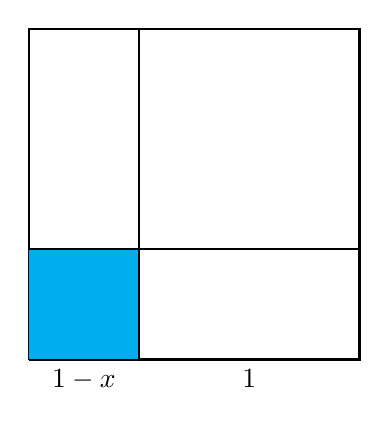
\begin{tikzpicture}[scale=.7]
            \draw [thick] (0,0) -- (2,0) -- (2,2) -- (0,2) -- (0,0);
            \draw [thick] (0,0) -- (6,0) -- (6,6) -- (0,6) -- (0,0);
            \draw [thick] (0,0) -- (2,0) -- (2,6) -- (0,6) -- (0,0);
            \draw [thick] (0,0) -- (6,0) -- (6,2) -- (0,2) -- (0,0);
            \draw [fill=cyan] (0,0) rectangle (2,2);
            \node [below] at (1,0) {$1-x$};
            \node [below] at (4,0) {$1$};
        \end{tikzpicture}
        \caption{$S$ 和网格不相交的充要条件}\label{f1.1}
    \end{figure}

    设方格的边长为 $x$, 则图 \ref{f1.1} 中的蓝色区域的边长为 $x-1$. $\because A$ 是在方格上随机取点, $\therefore A$ 落在蓝色区域的概率
    \[p=\dfrac{(x-1)^2}{x^2}\leq0.01.\]

    解得 $\dfrac{1}{11}\leq x\leq\dfrac{10}{9}$.

    当 $x\leq1$ 时硬币和网格一定相交, $\therefore$ 条件为 $1\leq x\leq\dfrac{10}{9}$.
\end{solution}
\begin{exercise}% 1.14
    在同一小时内有两辆汽车独立地到达同一个加油站加油, 车 $A$ 加油需要 $5\text{min}$, 车 $B$ 加油需要 $8\text{min}$. 如果每辆车在这一小时内等可能地到达, 计算这两辆汽车在加油站不能相遇的概率.
\end{exercise}
\begin{solution}
    设 $A,B$ 在加油站的时间分别为区间 $(x,x+5)$ 和 $(y,y+8)$, 如图 \ref{f1.2}.
    \begin{figure}[htbp!]
        \centering
        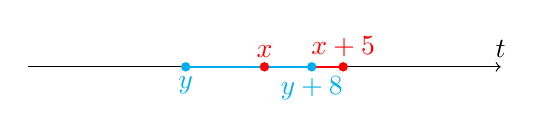
\begin{tikzpicture}[scale=.2]
            \draw [->] (0,0) -- (30,0);
            \draw [thick, red] (15,0) -- (20,0);
            \draw [thick, cyan] (10,0) -- (18,0);
            \fill [red] (15,0) circle [radius=.3];
            \fill [red] (20,0) circle [radius=.3];
            \fill [cyan] (10,0) circle [radius=.3];
            \fill [cyan] (18,0) circle [radius=.3];
            \node [above, red] at (15,0) {$x$};
            \node [above, red] at (20,0) {$x+5$};
            \node [below, cyan] at (10,0) {$y$};
            \node [below, cyan] at (18,0) {$y+8$};
            \node [above] at (30,0) {$t$};
        \end{tikzpicture}
        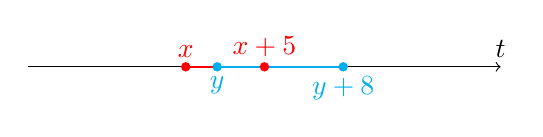
\begin{tikzpicture}[scale=.2]
            \draw [->] (0,0) -- (30,0);
            \draw [thick, red] (10,0) -- (15,0);
            \draw [thick, cyan] (12,0) -- (20,0);
            \fill [red] (10,0) circle [radius=.3];
            \fill [red] (15,0) circle [radius=.3];
            \fill [cyan] (12,0) circle [radius=.3];
            \fill [cyan] (20,0) circle [radius=.3];
            \node [above, red] at (10,0) {$x$};
            \node [above, red] at (15,0) {$x+5$};
            \node [below, cyan] at (12,0) {$y$};
            \node [below, cyan] at (20,0) {$y+8$};
            \node [above] at (30,0) {$t$};
        \end{tikzpicture}
        \caption{$A,B$ 在加油站相遇的两种情况, 红色表示 $A$, 蓝色表示 $B$}\label{f1.2}
    \end{figure}

    考虑两辆汽车在加油站相遇的情形会比较方便. 从图 \ref{f1.2} 可以看出要使得两辆汽车在加油站相遇, $A,B$ 到达加油站的时刻 $x,y$ 应满足以下条件\footnote{$\because$ 区域的边界的测度为 $0$, 不会影响概率, $\therefore$ 不用考虑是否取等号.}:
    \[\begin{cases}
        y+8>x, \\
        x+5>y. \\
    \end{cases}\]

    设 $\Omega=[0,60]^2$, $\Omega$ 中元素的第一个分量是 $A$ 到达加油站的时刻, 第二个分量是 $B$ 到达加油站的时刻.

    设事件 $C$ 表示两辆汽车在加油站相遇, 则 $C$ 对应的集合为
    \[\begin{cases}
        y+8>x, \\
        x+5>y, \\
        0<x<60, \\
        0<y<60. \\
    \end{cases}\]

    $C$ 对应的区域是图 \ref{f1.3} 中的蓝色区域, $\overline{C}$ 对应的区域是图 \ref{f1.3} 左上和右下的两个三角形.
    \begin{figure}[htbp!]
        \centering
        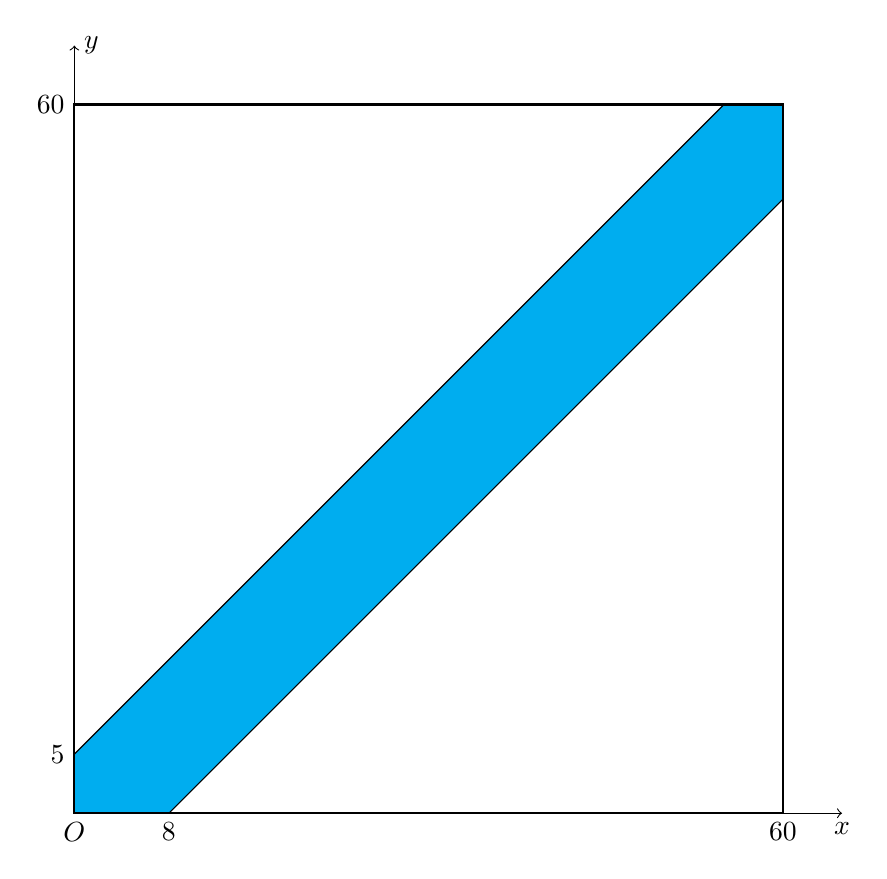
\begin{tikzpicture}[scale=.15]
            \draw [->] (0,0) -- (65,0);
            \draw [->] (0,0) -- (0,65);
            \draw [fill=cyan] (0,5) -- (55,60) -- (60,60) -- (60,52) -- (8,0) -- (0,0);
            \draw [thick] (0,0) rectangle (60,60);
            \node [below] at (0,0) {$O$};
            \node [below] at (65,0) {$x$};
            \node [below] at (8,0) {$8$};
            \node [below] at (60,0) {$60$};
            \node [right] at (0,65) {$y$};
            \node [left] at (0,5) {$5$};
            \node [left] at (0,60) {$60$};
        \end{tikzpicture}
        \caption{$C$ 对应的区域}\label{f1.3}
    \end{figure}

    $\therefore$
    \[P(\overline{C})=\dfrac{\dfrac{55^2}{2}+\dfrac{52^2}{2}}{60^2}\approx0.796.\]
\end{solution}
\addtocounter{exercise}{2}
\begin{exercise}% 1.17
    证明:
    \[P\left(\bigcup\limits_{j=1}^\infty A_j\right)\leq\sum\limits_{j=1}^\infty P(A_j).\]
\end{exercise}
\begin{proof}
    设 $A_0=\varnothing,B_j=A_j-\bigcup\limits_{i=1}^{j-1}A_i$.

    设 $\omega\in\bigcup\limits_{j=1}^\infty B_j$. 由式 (\ref{eq1.1}) 的定义, $\exists i\in\mathbb{N}_+$ 使得 $\omega\in B_i$.
    
    由 $B_i\subset A_i$ 得 $\omega\in A_i$. $\therefore\omega\in\bigcup\limits_{j=1}^\infty B_j$. $\therefore\bigcup\limits_{j=1}^\infty B_j\subset\bigcup\limits_{j=1}^\infty A_j$.

    设 $\omega\in\bigcup\limits_{j=1}^\infty A_j$. 由式 (\ref{eq1.1}) 的定义, $\exists i\in\mathbb{N}_+$ 使得 $\omega\in A_i$.
    
    $\therefore\exists k\in\mathbb{N}_+$ 使得 $\omega\in A_k$, 且 $\forall i<k,\omega\notin A_i$. $\therefore\omega\notin\bigcup\limits_{i=1}^{k-1}A_i$, $\therefore\omega\in B_k$. $\therefore\bigcup\limits_{j=1}^\infty A_j\subset\bigcup\limits_{j=1}^\infty B_j$.
    
    $\therefore\bigcup\limits_{j=1}^\infty A_j=\bigcup\limits_{j=1}^\infty B_j$. $\therefore$
    \[P\left(\bigcup\limits_{j=1}^\infty A_j\right)=P\left(\bigcup\limits_{j=1}^\infty B_j\right).\]

    $\because\forall j,k\in\mathbb{N}_+,B_j\subset A_j,B_{j+k}=A_{j+k}-\bigcup\limits_{i=1}^{j+k-1}A_i\subset  A_{j+k}-A_j$, $\therefore B_j,B_{j+k}$ 互不相容. 由可列可加性得
    \[P\left(\bigcup\limits_{j=1}^\infty B_j\right)=\sum\limits_{j=1}^\infty P(B_j).\]

    $\because B_j\subset A_j$, 由书上的定理 5.1 (5) 得 $P(B_j)<P(A_j)$, $\therefore$
    \[\sum\limits_{j=1}^\infty P(B_j)\leq\sum\limits_{j=1}^\infty P(A_j).\qedhere\]
\end{proof}
\begin{exercise}% 1.18
    设 $A_1,A_2,\cdots$ 的概率都为 $1$, 证明:
    \[P\left(\bigcap\limits_{j=1}^nA_j\right)=1,\quad P\left(\bigcap\limits_{j=1}^\infty A_j\right)=1.\]
\end{exercise}
\begin{proof}
    设 $B_i=\overline{A}_i$, 则 $B_1,B_2,\cdots$ 的概率都为 $0$.
    
    由书上的例 5.2 得
    \[P\left(\bigcup\limits_{j=1}^nB_j\right)=0,\quad P\left(\bigcup\limits_{j=1}^\infty B_j\right)=0.\]

    由书上的定理 5.1 (3) 得
    \[P\left(\overline{\bigcup\limits_{j=1}^nB_j}\right)=1,\quad P\left(\overline{\bigcup\limits_{j=1}^\infty B_j}\right)=1.\]

    由定理 \ref{t1.1} 得
    \[P\left(\bigcap\limits_{j=1}^nA_j\right)=P\left(\bigcap\limits_{j=1}^n\overline{B}_j\right)=P\left(\overline{\bigcup\limits_{j=1}^nB_j}\right)=1,\]
    \[P\left(\bigcap\limits_{j=1}^\infty A_j\right)=P\left(\bigcap\limits_{j=1}^\infty\overline{B}_j\right)=P\left(\overline{\bigcup\limits_{j=1}^\infty B_j}\right)=1.\qedhere\]
\end{proof}
\begin{exercise}\label{ex1.19}
    对于事件 $A,B$, 验证
    \[P(AB)+P(A\overline{B})+P(\overline{A}B)+P(\bar{A}\bar{B})=1.\]
\end{exercise}
\begin{proof}
    由定理 \ref{t1.2} 得
    \[\Omega=(A+\overline{A})(B+\overline{B})=AB+A\overline{B}+\overline{A}B+\bar{A}\bar{B}.\]

    容易验证 $AB,A\overline{B},\overline{A}B,\bar{A}\bar{B}$ 互不相容, 由可列可加性得
    \[1=P(\Omega)=P(AB)+P(A\overline{B})+P(\overline{A}B)+P(\bar{A}\bar{B}).\qedhere\]
\end{proof}
\section{第2章笔记}
补充几个定理的证明.
\begin{theorem}
    如果事件 $A$ 的概率为 $1$ 或 $0$, 则 $A$ 与任意事件 $B$ 相互独立.
\end{theorem}
\begin{proof}
    设 $P(A)=1$, 则由书上第 1 章的例 5.1 得 $P(AB)=P(B)=P(A)P(B)$, 即 $A,B$ 相互独立.

    设 $P(A)=0$, 则 $P(\overline{A})=1$, $\therefore\overline{A},B$ 相互独立, $\therefore A,B$ 相互独立.
\end{proof}
\begin{theorem}[Borel-Cantelli 引理]\label{t3.2}
    对事件列 $\{A_n\}$, 有:

    (1) 如果 $\sum\limits_{j=1}^\infty P(A_j)<\infty$, 则 $P\left(\bigcap\limits_{n=1}^\infty\bigcup\limits_{j=n}^\infty A_j\right)=0$;

    (2) 如果 $\{A_j\}$ 相互独立, $\sum\limits_{j=1}^\infty P(A_j)=\infty$, 则 $P\left(\bigcap\limits_{n=1}^\infty\bigcup\limits_{j=n}^\infty A_j\right)=1$.
\end{theorem}
\begin{proof}
    (1) 令 $C_n=\bigcup\limits_{j=n}^\infty A_j$, 则 $C_n$ 是单调减的, 由书上第 1 章的定理 6.1 得
    \[P\left(\bigcap\limits_{n=1}^\infty\bigcup\limits_{j=n}^\infty A_j\right)=P\left(\bigcap\limits_{n=1}^\infty C_j\right)=\lim\limits_{n\to\infty}P(C_n).\]

    由书上第 1 章的定理 5.1 (6) 得
    \[\lim\limits_{n\to\infty}P(C_n)=\lim\limits_{n\to\infty}P\left(\bigcup\limits_{j=n}^\infty A_j\right)\leq\lim\limits_{n\to\infty}\sum\limits_{j=n}^\infty P(A_j).\]

    $\because\sum\limits_{j=1}^\infty P(A_j)<\infty$, $\therefore\sum\limits_{j=n}^\infty P(A_j)\to0(n\to\infty)$. $\therefore\lim\limits_{n\to\infty}P(C_n)=0$.

    (2) 与 (1) 一样, 有
    \[P\left(\bigcap\limits_{n=1}^\infty\bigcup\limits_{j=n}^\infty A_j\right)=\lim\limits_{n\to\infty}P\left(\bigcup\limits_{j=n}^\infty A_j\right).\]
    
    由定理 \ref{t1.3} 得
    \[\lim\limits_{n\to\infty}P\left(\bigcup\limits_{j=n}^\infty A_j\right)=\lim\limits_{n\to\infty}\lim\limits_{m\to\infty}P\left(\bigcup\limits_{j=n}^mA_j\right).\]

    由定理 \ref{t1.1} 得
    \begin{align*}
        \lim\limits_{n\to\infty}\lim\limits_{m\to\infty}P\left(\bigcup\limits_{j=n}^mA_j\right) & =\lim\limits_{n\to\infty}\lim\limits_{m\to\infty}\left(1-P\left(\bigcap\limits_{j=n}^m\overline{A}_j\right)\right) \\
        & =\lim\limits_{n\to\infty}\left(1-\lim\limits_{m\to\infty}P\left(\bigcap\limits_{j=n}^m\overline{A}_j\right)\right).
    \end{align*}

    由书上的例 2.5 (2) 得 $\overline{A}_j$ 相互独立. $\therefore$
    \begin{align*}
        \lim\limits_{n\to\infty}\left(1-\lim\limits_{m\to\infty}P\left(\bigcap\limits_{j=n}^m\overline{A}_j\right)\right) & =\lim\limits_{n\to\infty}\left(1-\lim\limits_{m\to\infty}\prod\limits_{j=n}^mP(\overline{A}_j)\right) \\
        & =\lim\limits_{n\to\infty}\left(1-\lim\limits_{m\to\infty}\prod\limits_{j=n}^m(1-P(A_j))\right).
    \end{align*}

    $\because\forall x>0,1-x\leq e^{-x}$, $\therefore$
    \begin{align*}
        \lim\limits_{n\to\infty}\left(1-\lim\limits_{m\to\infty}\prod\limits_{j=n}^m(1-P(A_j))\right) & \leq\lim\limits_{n\to\infty}\left(1-\lim\limits_{m\to\infty}\prod\limits_{j=n}^m\exp(-P(A_j))\right) \\
        & =\lim\limits_{n\to\infty}\left(1-\lim\limits_{m\to\infty}\exp\left(-\sum\limits_{j=n}^mP(A_j)\right)\right) \\
        & =\lim\limits_{n\to\infty}\left(1-\exp\left(-\lim\limits_{m\to\infty}\sum\limits_{j=n}^mP(A_j)\right)\right) \\
        & =\lim\limits_{n\to\infty}\left(1-\exp\left(-\sum\limits_{j=n}^\infty P(A_j)\right)\right).
    \end{align*}

    $\because\forall n,\sum\limits_{j=n}^\infty P(A_j)=\infty$, $\therefore\forall n,\exp\left(-\sum\limits_{j=n}^\infty P(A_j)\right)=0$. $\therefore$
    \[\lim\limits_{n\to\infty}\left(1-\exp\left(-\sum\limits_{j=n}^\infty P(A_j)\right)\right)=\lim\limits_{n\to\infty}(1-0)=1.\qedhere\]
\end{proof}
在第 (2) 条中有 $\{A_j\}$ 相互独立的条件. 下面的例子说明, 如果 $\{A_j\}$ 不相互独立, 则 Borel-Cantelli 引理不一定成立.

\section{第2章习题}
\addtocounter{exsection}{2}
\addtocounter{exercise}{9}
\begin{exercise}% 2.11
    某人参加微积分和线性代数的考试, 无论哪门课先考, 微积分和线性代数通过的概率分别是 $a,b$, 在微积分先考并通过的条件下, 线性代数通过的概率是 $c$. 当微积分先考时, 计算

    (a) 两门课都通过的概率;

    (b) 微积分没通过的条件下, 线性代数通过的概率;

    (d) 至少一门通过的概率;

    (e) 至少一门不通过的概率.
\end{exercise}
\begin{solution}
    设``微积分通过''和``线性代数通过''的事件分别为 $A,B$, ``微积分先考''的事件为 $C$, 则 $P_C(A)=P_{\overline{C}}(A)=a,P_C(B)=P_{\overline{C}}(B)=b,P_C(B|A)=P(B|AC)=c$.

    (a) ``两门课都通过''的事件为 $AB$. 有 $P_C(AB)=P_C(B|A)P_C(A)=ac$.

    (b) ``微积分没通过的条件下, 线性代数通过''的事件为 $B|\overline{A}$. 由全概率公式,
    \[P_C(B)=P_C(B|A)P_C(A)+P_C(B|\overline{A})P_C(\overline{A})=ac+(1-a)P_C(B|\overline{A}).\]

    $\therefore$
    \[P_C(B|\overline{A})=\dfrac{b-ac}{1-a}.\]

    (d) 设``至少一门通过''的事件为 $C$, 则 $\overline{C}=\bar{A}\bar{B}$. 有
    \begin{align*}
        P_C(C) & =1-P_C(\bar{A}\bar{B}) \\
        & =1-P_C(\overline{B}|\overline{A})P_C(\overline{A}) \\
        & =1-(1-P_C(B|\overline{A}))P_C(\overline{A}) \\
        & =a+b-ac.
    \end{align*}
\end{solution}
\stepcounter{exercise}
\begin{exercise}% 2.12
    投 $2$ 个均匀的骰子, 已知至少有一个骰子的点数是 $3$.

    (a) 计算这两个骰子的点数之和为 $7$ 的概率;
    
    (b) 两个骰子的点数之和更有可能是 $7$ 还是 $6$?
\end{exercise}
\begin{solution}
    (a) 设``第一个骰子的点数为 $i$''的事件为 $A_i$, ``第二个骰子的点数为 $i$''的事件为 $B_i$, 则``至少有一个骰子的点数是 $3$''的事件为 $A_3\cup B_3$. 由加法公式,
    \[P(A_3\cup B_3)=P(A_3)+P(B_3)-P(A_3B_3)=\dfrac{1}{6}+\dfrac{1}{6}-\dfrac{1}{36}=\dfrac{11}{36}.\]

    ``两个骰子的点数之和为 $7$ 的概率''的事件为 $A_3B_4+A_4B_3$, 概率为 $\dfrac{2}{36}$.

    $\therefore$ 已知至少有一个骰子的点数是 $3$ 的情况下, 两个骰子的点数之和为 $7$ 的概率为 $\dfrac{2/36}{11/36}=\dfrac{2}{11}$.

    (b) ``两个骰子的点数之和为 $6$ 的概率''的事件为 $A_3B_3$, 概率为 $\dfrac{1}{36}$.

    $\therefore$ 已知至少有一个骰子的点数是 $3$ 的情况下, 两个骰子的点数之和为 $6$ 的概率为 $\dfrac{1/36}{11/36}=\dfrac{1}{11}\leq\dfrac{2}{11}$. $\therefore$ 两个骰子的点数之和更有可能是 $7$.
\end{solution}

可以用两种不同的方式来看待条件概率, 一种是作为条件的事件 $C$ 改变了样本空间 $\Omega$, 另一种是 $C$ 没有改变 $\Omega$, 但改变了 $\mathcal{F}$ 上的概率(从原来的 $P$ 变为 $P_C$). 我们通常采用后一种看法, 但有时前一种看法会更方便.
\begin{solution}[另一种解法]
    用 $(a,b)$ 来表示一次试验, 含义是``第一个骰子的点数为 $a$, 第二个骰子的点数为 $b$.''已知至少有一个骰子的点数是 $3$ 的情况下, 样本空间 $\Omega=\{(1,3),(2,3),\cdots,(6,3),(3,1),(3,2),\cdots,(3,6)\}$, $^\#\Omega=11$(注意 $(3,3)$ 只计算了一次).

    ``两个骰子的点数之和为 $7$ 的概率''的事件为 $\{(3,4),(4,3)\}$, $P(\{(3,4),(4,3)\})=\dfrac{2}{11}$, ``两个骰子的点数之和为 $6$ 的概率''的事件为 $\{(3,3)\}$, $P(\{(3,3)\})=\dfrac{1}{11}$.
\end{solution}
\addtocounter{exercise}{6}
\begin{exercise}% 2.19
    甲和另一人下棋, 每局有甲输, 甲赢, 平局三种结果, 每局获胜者得 $1$ 分, 累积多于对手 $2$ 分者获胜. 设每局的结果相互独立, 甲每局获胜的概率为 $p$, 求甲最终获胜的概率.
\end{exercise}
\begin{solution}
    设``甲在某一局获胜'', ``某一局是平局'', ``甲在某一局没获胜''的事件分别为 $A_1,A_2,A_3$, ``某一局前甲比对手多 $k$ 分且甲最终获胜''的事件为 $B_k$. 由全概率公式,
    \[P(B_k)=P(B_k|A_1)P(A_1)+P(B_k|A_2)P(A_2)+P(B_k|A_3)P(A_3).\]

    设 $r=P(A_3)$, $q(k)=P(B_k)$, 则 $q(-2)=0,q(2)=1$, 甲最终获胜的概率为 $q(0)$.
    \[q(k)=q(k+1)p+q(k)(1-p-r)+q(k-1)r.\]

    $\therefore$
    \[q(k)=\dfrac{p}{p+r}q(k+1)+\dfrac{r}{p+r}q(k-1).\]

    代入得
    \begin{align*}
        q(0) & =\dfrac{p}{p+r}q(1)+\dfrac{r}{p+r}q(-1) \\
        & =\dfrac{p}{p+r}\left(\dfrac{p}{p+r}q(2)+\dfrac{r}{p+r}q(0)\right)+\dfrac{r}{p+r}\left(\dfrac{p}{p+r}q(0)+\dfrac{r}{p+r}q(-2)\right) \\
        & =\dfrac{p}{p+r}\left(\dfrac{p}{p+r}+\dfrac{r}{p+r}q(0)\right)+\dfrac{r}{p+r}\cdot\dfrac{p}{p+r}q(0) \\
        & =\dfrac{p^2}{(p+r)^2}+\dfrac{2pr}{(p+r)^2}q(0).
    \end{align*}

    解得
    \[q(0)=\dfrac{p^2}{p^2+r^2}.\]
\end{solution}
\begin{exercise}% 2.20
    用红, 黑两种药治疗同一种疾病, 为了决定用哪种药, 医生将口袋中放入 $r$ 个红球和 $b$ 个黑球后任取一个球, 取到黑球用黑药, 并将球放回, 取到红球用红药, 并将球放回. 如果药物有效就加入一个相同颜色的球. 用 $B_i$ 表示第 $i$ 次取球时取到黑球, 设两种药都一定有效.

    (b) 计算 $P(B_2),P(B_3)$;

    (c) 计算 $P(B_n)$.
\end{exercise}
\begin{solution}
    (b)
    \begin{align*}
        P(B_2) & =P(B_2|B_1)P(B_1)+P(B_2|\overline{B}_1)P(\overline{B}_1) \\
        & =\dfrac{b+1}{r+b+1}\cdot\dfrac{b}{r+b}+\dfrac{b}{r+b+1}\cdot\dfrac{r}{r+b} \\
        & =\dfrac{b(r+b+1)}{(r+b+1)(r+b)}=\dfrac{b}{r+b}.
    \end{align*}

    由第 \ref{ex1.19} 题得 $B_1B_2,B_1\overline{B}_2,\overline{B}_1B_2,\overline{B}_1\overline{B}_2$ 是完备事件组. 由全概率公式,
    \begin{align*}
        P(B_3) & =P(B_3|B_1B_2)P(B_1B_2)+P(B_3|B_1\overline{B}_2)P(B_1\overline{B}_2) \\
        &\ +P(B_3|\overline{B}_1B_2)P(\overline{B}_1B_2)+P(B_3|\overline{B}_1\overline{B}_2)P(\overline{B}_1\overline{B}_2) \\
        & =P(B_3|B_1B_2)P(B_2|B_1)P(B_1)+P(B_3|B_1\overline{B}_2)P(\overline{B}_2|B_1)P(B_1) \\
        &\ +P(B_3|\overline{B}_1B_2)P(B_2|\overline{B}_1)P(\overline{B}_1)+P(B_3|\overline{B}_1\overline{B}_2)P(\overline{B}_2|\overline{B}_1)P(\overline{B}_1) \\
        & =\dfrac{b+2}{r+b+2}\cdot\dfrac{b+1}{r+b+1}\cdot\dfrac{b}{r+b}+\dfrac{b+1}{r+b+1}\cdot\dfrac{r}{r+b+1}\cdot\dfrac{b}{r+b} \\
        &\ +\dfrac{b+1}{r+b+2}\cdot\dfrac{b}{r+b+1}\cdot\dfrac{r}{r+b}+\dfrac{b}{r+b+2}\cdot\dfrac{r+1}{r+b+1}\cdot\dfrac{r}{r+b} \\
        & =\dfrac{(b+2)(b+1)b+2(b+1)br+(r+1)rb}{(r+b+2)(r+b+1)(r+b)} \\
        & =b\cdot\dfrac{b^2+3b+2+2br+2r+r^2+r}{(r+b+2)(r+b+1)(r+b)}=\dfrac{b}{r+b}.
    \end{align*}

    (c) $P(B_n)=\dfrac{b}{r+b}$. $n=1$ 的情形是显然的.

    假设 $P(B_{n-1})=\dfrac{b}{r+b}$. 如果开始时口袋中有 $r'$ 个红球和 $b'$ 个黑球, 那么第 $n-1$ 次取球时取到黑球的概率为 $\dfrac{b'}{r'+b'}$.

    可以认为试验是从第 $2$ 次取球时开始的, 这时第 $n-1$ 次取球时取到黑球对应事件 $B_n|B_1$ 或 $B_n|\overline{B}_1$. 如果第 $1$ 次取球时取到黑球, 那么试验开始时口袋中有 $r$ 个红球和 $b+1$ 个黑球; 如果第 $1$ 次取球时取到红球, 那么试验开始时口袋中有 $r+1$ 个红球和 $b$ 个黑球. $\therefore$
    \[P(B_n|B_1)=\dfrac{b+1}{r+b+1},\quad P(B_n|\overline{B}_1)=\dfrac{b}{r+b+1}.\]

    由全概率公式得
    \begin{align*}
        P(B_n) & =P(B_n|B_1)P(B_1)+P(B_n|\overline{B}_1)P(\overline{B}_1) \\
        & =\dfrac{b+1}{r+b+1}\cdot\dfrac{b}{r+b}+\dfrac{b}{r+b+1}\cdot\dfrac{r}{r+b} \\
        & =\dfrac{b}{r+b}.
    \end{align*}
\end{solution}
\addtocounter{exercise}{7}
\begin{exercise}\label{ex2.28}
    口袋中有一个红球和一个黑球, 每次从口袋中有放回地任取一个球, 且第 $j$ 次取球后再加入 $j$ 个红球. 如果一直做下去, 能够取到黑球多少次?
\end{exercise}
\begin{solution}
    用 $A_j$ 表示第 $j$ 次取球时取到黑球. 第 $j$ 次取球时口袋中有 $2+\sum\limits_{i=1}^{j-1}i=2+\dfrac{j(j-1)}{2}$ 个球. $\therefore$
    \[P(A_j)=\dfrac{1}{2+\dfrac{j(j-1)}{2}}.\]

    $\because\lim\limits_{j\to\infty}\dfrac{P(A_j)}{1/j^2}=1$ 而 $\sum\limits_{j=1}^\infty\dfrac{1}{j^2}<\infty$, $\therefore\sum\limits_{j=1}^\infty P(A_j)<\infty$, 由定理 \ref{t3.2} 得 $P\left(\bigcap\limits_{n=1}^\infty\bigcup\limits_{j=n}^\infty A_j\right)=0$, 即只有有限次取到黑球.
\end{solution}
\begin{exercise}% 2.29
    在习题 \ref{ex2.28} 中, 若第 $j$ 次取球后再加入 $j$ 个红球和 $1$ 个黑球, 能够取到黑球多少次?
\end{exercise}
\begin{solution}
    用 $A_j$ 表示第 $j$ 次取球时取到黑球. 第 $j$ 次取球时口袋中有 $2+(j-1)+\sum\limits_{i=1}^{j-1}i=1+\dfrac{j(j+1)}{2}$ 个球, 其中 $j-1$ 个是黑球. $\therefore$
    \[P(A_j)=\dfrac{j-1}{1+\dfrac{j(j+1)}{2}}.\]

    $\because\lim\limits_{j\to\infty}\dfrac{P(A_j)}{1/j}=1$ 而 $\sum\limits_{j=1}^\infty\dfrac{1}{j}=\infty$, $\therefore\sum\limits_{j=1}^\infty P(A_j)=\infty$, 由定理 \ref{t3.2} 得 $P\left(\bigcap\limits_{n=1}^\infty\bigcup\limits_{j=n}^\infty A_j\right)=1$, 即有无限次取到黑球.
\end{solution}
\begin{exercise}\label{ex2.30}
    证明全概率公式: 如果事件 $A_1,A_2,\cdots$ 互不相容, $B\subset\bigcup\limits_{j=1}^\infty A_j$, 则
    \[P(B)=\sum\limits_{j=1}^\infty P(A_j)P(B|A_j).\]
\end{exercise}
\begin{proof}
    设 $\omega\in B\cap\left(\bigcup\limits_{j=1}^\infty A_j\right)$, 则 $\omega\in B$ 且 $\exists j\in\mathbb{N},\omega\in A_j$. $\therefore\exists j\in\mathbb{N},\omega\in A_jB$. $\therefore B\cap\left(\bigcup\limits_{j=1}^\infty A_j\right)=\bigcup\limits_{j=1}^\infty A_jB$

    由定理 \ref{t1.2} 得
    \[B\cap\left(\bigcup\limits_{j=1}^\infty A_j\right)=\bigcup\limits_{j=1}^\infty A_jB.\]

    $\because A_1,A_2,\cdots$ 互不相容, $\therefore A_1B,A_2B,\cdots$ 互不相容. 由书上第 1 章的定义 4.1(c) 得
    \[P(B)=P\left(\bigcup\limits_{j=1}^\infty A_jB\right)=\sum\limits_{j=1}^\infty P(A_jB).\]

    由乘法公式得
    \[\sum\limits_{j=1}^\infty P(A_jB)=\sum\limits_{j=1}^\infty P(B|A_j)P(A_j).\]
\end{proof}
\begin{exercise}% 2.31
    证明 Bayes 公式: 如果事件 $A_1,A_2,\cdots$ 互不相容, $B\subset\bigcup\limits_{j=1}^\infty A_j$, 则 $P(B)>0$ 时有
    \[P(A_j|B)=\dfrac{P(A_j)P(B|A_j)}{\sum\limits_{i=1}^\infty P(A_i)P(B|A_i)},\quad j\geq1.\]
\end{exercise}
\begin{proof}
    由乘法公式得
    \[P(A_j|B)=\dfrac{P(A_jB)}{P(B)}=\dfrac{P(B|A_j)P(A_j)}{P(B)}.\]

    由第 \ref{ex2.30} 得
    \[\dfrac{P(B|A_j)P(A_j)}{P(B)}=\dfrac{P(B|A_j)P(A_j)}{\sum\limits_{i=1}^\infty P(A_i)P(B|A_i)}.\qedhere\]
\end{proof}
\stepcounter{exercise}
\begin{exercise}% 2.33
    如果你的水平略高于对手, 为了保证比赛获胜, 你期望比赛规则是三局两胜还是五局三胜?
\end{exercise}
\begin{solution}
    见 \url{http://lanqi.org/everyday/19943/}.
\end{solution}
\stepcounter{exercise}
\begin{exercise}% 2.35
    设想如下的抽奖节目: 三扇关闭的门后各有一个奖品, 其中之一是汽车, 其余是羊. 每扇门后是汽车的概率相同. 猜奖者任选一扇门后得到门后的奖品. 当猜奖者选中一扇门尚未打开时, 主持人打开了另外两扇门之一, 发现门后是羊. 这时猜奖者有机会改猜剩下的那扇门. 在下面的情况下, 计算猜奖者换门或不换门得到汽车的概率:

    (a) 假设主持人知道汽车在哪扇门后;

    (b) 假设主持人不知道汽车在哪扇门后;

    (c) 假设主持人知道汽车在哪扇门后的概率为 $0.6$.
\end{exercise}
\begin{solution}
    称猜奖者一开始选中的门是``$1$ 号门'', 主持人打开的门是``$2$ 号门'', 剩下的那扇门是``$3$ 号门'', $A_i\ (i=1,2,3)$ 表示事件``汽车在 $i$ 号门后'', $B$ 表示事件``主持人打开 $2$ 号门, 发现门后是羊''. 要求 $P(A_1|B)$ 和 $P(A_3|B)$. 由 Bayes 公式得
    \[P(A_i|B)=\dfrac{P(B|A_i)P(A_i)}{\sum\limits_{j=1}^3P(B|A_j)P(A_j)}.\]

    $\because P(A_1)=P(A_2)=P(A_3)=\dfrac{1}{3}$, $\therefore$
    \[P(A_i|B)=\dfrac{P(B|A_i)}{\sum\limits_{j=1}^3P(B|A_j)}.\]

    首先, ``主持人打开 $2$ 号门, 发现门后是羊''意味着车不可能在 $2$ 号门后, 即 $P(B|A_2)=0$. 其余的条件概率会随情况而变化.

    (a) 如果汽车在 $1$ 号门后, 那么主持人可以从 $2$ 号和 $3$ 号门中任选一扇打开, $\therefore P(B|A_1)=\dfrac{1}{2}$.

    如果汽车在 $3$ 号门后, 那么主持人一定会打开 $2$ 号门, $\therefore P(B|A_3)=1$. $\therefore$
    \[P(A_1|B)=\dfrac{\dfrac{1}{2}}{\dfrac{1}{2}+1}=\dfrac{1}{3},\quad P(A_3|B)=\dfrac{1}{\dfrac{1}{2}+1}=\dfrac{2}{3}.\]

    (b) $\because$ 主持人不知道汽车在哪扇门后, $\therefore$ 无论汽车在哪扇门后, 主持人都会从 $2$ 号和 $3$ 号门中任选一扇打开, $\therefore P(B|A_1)=P(B|A_3)=\dfrac{1}{2}$. $\therefore P(A_1|B)=P(A_3|B)=\dfrac{1}{2}$.

    (c) 设``主持人知道汽车在哪扇门后''为事件 $C$, 则由 (a) 得 $P_C(B|A_1)=\dfrac{1}{2},P_C(B|A_3)=1$, 由 (b) 得 $P_{\overline{C}}(B|A_1)=P_{\overline{C}}(B|A_3)=\dfrac{1}{2}$. 由全概率公式得
    \[P(B|A_1)=P_C(B|A_1)P(C)+P_{\overline{C}}(B|A_1)P(\overline{C})=\dfrac{1}{2},\]
    \[P(B|A_3)=P_C(B|A_3)P(C)+P_{\overline{C}}(B|A_3)P(\overline{C})=\dfrac{4}{5}.\]

    $\therefore$
    \[P(A_1|B)=\dfrac{\dfrac{1}{2}}{\dfrac{1}{2}+\dfrac{4}{5}}=\dfrac{5}{13},\quad P(A_3|B)=\dfrac{\dfrac{4}{5}}{\dfrac{1}{2}+\dfrac{4}{5}}=\dfrac{8}{13}.\]
\end{solution}
\begin{exercise}
    在书上的例 1.4 中, 当全班有 $n$ 个人时, 用 $B_n$ 表示至少有一人得到自己的作业本, 用 $D_k$ 表示恰好有 $k$ 个人得到自己的作业本, 计算 $^\#\overline{B}_n$ 和 $P(D_k)$.
\end{exercise}
\begin{solution}
    由书上的例 1.4 得 $P(B_n)=\sum\limits_{k=1}^n(-1)^{k-1}\dfrac{1}{k!}$. $\therefore$
    \[P(\overline{B}_n)=1-P(B_n)=\sum\limits_{i=0}^n(-1)^{i}\dfrac{1}{i!}.\]

    $\therefore$
    \[^\#\overline{B}_n=^\#\Omega P(\overline{B}_n)=n!\sum\limits_{i=0}^n(-1)^{i}\dfrac{1}{i!}.\]
    
    $\overline{B}_{n-k}$ 表示``把 $n-k$ 个作业本随机分给 $n-k$ 个人, 没有人得到自己的作业本''. 恰好有 $k$ 个人得到自己的作业本意味着剩下 $n-k$ 个人中没有人得到自己的作业本. $\therefore$
    \[D_k=\sum\limits_{1\leq j_1<j_2<\cdots<j_k\leq n}A_{j_1}A_{j_2}\cdots A_{j_k}\overline{B}_{n-k},\]
    \[P(D_k)=C_n^k\dfrac{(n-k)!}{n!}P(\overline{B}_{n-k})=\dfrac{1}{k!}\sum\limits_{i=0}^{n-k}(-1)^{i}\dfrac{1}{i!}.\]
\end{solution}
\section{第3章笔记}
为了引入随机变量的定义, 首先需要介绍一些测度论的概念.
\begin{definition}
    设 $\Omega$ 是任意的集合, $\mathcal{F}$ 是 $\Omega$ 上的 $\sigma$ 域($\mathcal{F}$ 是 $\Omega$ 的子集构成的集合且 $\mathcal{F}$ 满足书上第 1 章第 4 节开头的条件), 则称 $(\Omega,\mathcal{F})$ 是一个\textbf{可测空间}.
\end{definition}
\begin{definition}
    设 $(\Omega_1,\mathcal{F}_1),(\Omega_2,\mathcal{F}_2)$ 是两个可测空间, 如果函数 $f:\Omega_1\to\Omega_2$ 满足: $\forall A\in\mathcal{F}_2$, $f$ 在 $A$ 上的原像 $\{\omega|f(\omega)\in A\}\in\mathcal{F}_1$, 则称 $f$ 是一个\textbf{可测变换}.
\end{definition}

从概率空间 $(\Omega,\mathcal{F},P)$ 可以自然地得到一个可测空间 $(\Omega,\mathcal{F})$. 设 $\mathcal{R}$ 是包含 $\mathbb{R}$ 上的区间全体的 $\sigma$ 域. 按照定义, $(\mathbb{R},\mathcal{R})$ 是一个可测空间, 称为 \textbf{Borel 可测集}. 有:
\begin{definition}
    设 $(\Omega,\mathcal{F},P)$ 是概率空间, $(\mathbb{R},\mathcal{R})$ 是 Borel 可测集, 称可测变换 $X:\Omega\to\mathbb{R}$ 是 $\Omega$ 上的\textbf{随机变量}.
\end{definition}

在初等概率论中, 可以简单地认为 $\Omega$ 上的随机变量是 $\Omega$ 上的实值函数.
\begin{example}[书上的例 1.3(2)]
    设 $X$ 是随机变量, $x\in\mathbb{R}$, 则
    \[\bigcup\limits_{n=1}^\infty\{X\leq x-1/n\}=\{X<x\}.\]
\end{example}
\begin{proof}
    设 $\omega\in\bigcup\limits_{n=1}^\infty\{X\leq x-1/n\}$, 则 $\exists m\in\mathbb{N}_+,X(\omega)\leq x-\dfrac{1}{m}<x$. $\therefore\omega\in\{X<x\}$. $\therefore\bigcup\limits_{n=1}^\infty\{X\leq x-1/n\}\subset\{X<x\}$.

    设 $\omega\in\{X<x\}$, 则 $\exists\varepsilon>0$ 使得 $X(\omega)\leq x-\varepsilon$. 取 $m\geq\dfrac{1}{\varepsilon}$, 则 $\omega\in\{X\leq x-1/m\}$. $\therefore\omega\in\bigcup\limits_{n=1}^\infty\{X\leq x-1/n\}$. $\therefore\bigcup\limits_{n=1}^\infty\{X\leq x-1/n\}\supset\{X<x\}$.
\end{proof}

随机变量 $X$ 可以由其分布函数 $F(x)=P(X\leq x)$ 唯一确定. 之后用 $X\sim F(x)$ 来表示由 $F(x)$ 确定的随机变量.
\section{第3章习题}
\addtocounter{exsection}{3}
\begin{exercise}% 3.1
    证明:
    \[\lim\limits_{x\to\infty}F(x)=1,\quad\lim\limits_{x\to-\infty}F(x)=0.\]
\end{exercise}
\begin{proof}
    $\because\lim\limits_{x\to\infty}F(x)$ 存在, $\therefore\lim\limits_{x\to\infty}F(x)=\lim\limits_{n\to\infty}F(n)=\lim\limits_{n\to\infty}P(X\leq n)$.

    $\because\{X\leq n\}$ 单调递增, 由概率的连续性得
    \[\lim\limits_{n\to\infty}P(X\leq n)=P\left(\bigcup\limits_{n=1}^\infty\{X\leq n\}\right)=P(X<\infty)=1.\]

    $\because\lim\limits_{x\to-\infty}F(x)$ 存在, $\therefore\lim\limits_{x\to-\infty}F(x)=\lim\limits_{n\to\infty}F(-n)=\lim\limits_{n\to\infty}P(X\leq-n)$.

    $\because\{X\leq-n\}$ 单调递减, 由概率的连续性得
    \[\lim\limits_{n\to\infty}P(X\leq-n)=P\left(\bigcap\limits_{n=1}^\infty\{X\leq-n\}\right)=P(X\leq-\infty)=0.\qedhere\]
\end{proof}
\begin{exercise}% 3.2
    证明: 如果常数 $a,b,c$ 使得 $g(x)=\exp(ax^2+bx+c),x\in\mathbb{R}$ 是概率密度, 则 $a<0$.
\end{exercise}
\begin{proof}
    证明逆否命题. 若 $a=0$, 则 $g(x)=e^{bx+c}$, $\because g$ 在 $\mathbb{R}$ 上不可积, $\therefore g$ 不是概率密度.
    
    若 $a>0$, 则 $g(x)=\exp\left(a\left(x+\dfrac{b}{2a}\right)^2-\dfrac{b^2}{4a^2}+c\right)$. $\because g(x)\to\infty\ (x\to\pm\infty)$, $\therefore g$ 在 $\mathbb{R}$ 上不可积, $\therefore g$ 不是概率密度.
\end{proof}
\addtocounter{exercise}{6}
\begin{exercise}% 3.9
    甲每天收到的电子邮件数服从 Poisson 分布 $\mathcal{P}(\lambda)$, 且每封电子邮件被过滤掉的概率为 $0.2$.

    (c) 已知甲看到了自己的 $k$ 封电子邮件, 计算他有 $m$ 封电子邮件被过滤掉的概率.

    (d) 甲每天看到的电子邮件数与被过滤掉的电子邮件数是否独立?
\end{exercise}
\begin{solution}
    (c) 设 $A_k$ 表示事件``甲看到了 $k$ 封电子邮件'',  $B_m$ 表示事件``甲有 $m$ 封电子邮件被过滤掉'', 则事件 $A_kB_m$ 意味着甲一共收到了 $k+m$ 封电子邮件. $\therefore$
    \[P(A_kB_m)=\dfrac{\lambda^{k+m}}{(k+m)!}e^{-\lambda}\cdot C_{k+m}^k\cdot0.8^k\cdot0.2^m.\]

    由书上的例 2.3 得甲每天看到的电子邮件数服从 Poisson 分布 $\mathcal{P}(0.8\lambda)$. 有
    \begin{align*}
        P(B_m|A_k) & =\dfrac{P(A_kB_m)}{P(A_k)} \\
        & =\dfrac{\dfrac{\lambda^{k+m}}{(k+m)!}e^{-\lambda}\cdot C_{k+m}^k\cdot0.8^k\cdot0.2^m}{\dfrac{(0.8\lambda)^k}{k!}e^{-0.8\lambda}} \\
        & =\dfrac{\lambda^m}{m!}e^{-0.2\lambda}\cdot0.2^m.
    \end{align*}

    (d) 由书上的例 2.3 得甲每天被过滤掉的电子邮件数服从 Poisson 分布 $\mathcal{P}(0.2\lambda)$. 有
    \[P(B_m)=\dfrac{(0.2\lambda)^m}{m!}e^{-0.2\lambda}=P(B_m|A_k).\]

    $\therefore$ 甲每天看到的电子邮件数与被过滤掉的电子邮件数相互独立.
\end{solution}
\begin{exercise}% 3.10
    设车间有 $100$ 台型号相同的机床相互独立地工作, 每台机床在时间 $(0,t]$ 内发生故障的概率为 $0.01$, 发生故障的机床需要一人来维修, 且一人在 $(0,t]$ 内只能维修一台机床. 考虑两种配备维修工人的方法:

    (a) $5$ 个人每人负责 $20$ 台机床.
    
    (b) $3$ 个人同时负责 $100$ 台机床.

    在以上两种情况下计算机床在时间 $(0,t]$ 内发生故障时不能被及时维修的概率.
\end{exercise}
\begin{solution}
    (a) 考虑 $5$ 个维修工人中的任意一个(记为工人甲). 工人甲负责的机床中发生故障的机床数 $n$ 服从二项分布 $\mathcal{B}(20,0.01)$, 他能及时维修这 $20$ 台机床的概率为 $P(n\leq1)=0.99^{20}+C_{20}^1\cdot0.99^{19}\cdot0.01\approx0.98314$.

    $\therefore$ 全部 $100$ 台机床在时间 $(0,t]$ 内发生故障时不能被及时维修的概率为 $1-0.98314^5\approx0.0815$.

    (b) $100$ 台机床中发生故障的机床数 $n$ 服从二项分布 $\mathcal{B}(100,0.01)$. 机床在时间 $(0,t]$ 内发生故障时不能被及时维修的概率为
    \begin{align*}
        1-P(n\leq 3) & =1-(0.99^{100}+C_{100}^1\cdot0.99^{99}\cdot0.01+C_{100}^2\cdot0.99^{98}\cdot0.01^2+C_{100}^3\cdot0.99^{97}\cdot0.01^3) \\
        & \approx0.0184.
    \end{align*}
\end{solution}
\addtocounter{exercise}{3}
\begin{exercise}% 3.14
    一个使用了 $t$ 小时的电阻在 $\Delta t$ 内失效的概率是 $\lambda\Delta t+o(\Delta t)$, 设该电阻的使用寿命是连续型随机变量 $X$, 求 $X$ 的分布.
\end{exercise}
\begin{solution}
    该电阻在 $\Delta t$ 内不失效的概率是 $1-\lambda\Delta t-o(\Delta t)$, $\therefore$
    \[P(X>t+\Delta t|X>t)=1-\lambda\Delta t-o(\Delta t).\]

    $\therefore$
    \[P(X>t+\Delta t)=(1-\lambda\Delta t-o(\Delta t))P(X>t).\]

    设 $X$ 的分布函数为 $F(x)$, 则
    \begin{align*}
        F(t+\Delta t) & =1-P(X>t+\Delta t) \\
        & =1-(1-\lambda\Delta t-o(\Delta t))P(X>t) \\
        & =1-(1-\lambda\Delta t-o(\Delta t))(1-F(t)) \\
        & =(\lambda\Delta t+o(\Delta t))(1-F(t))+F(t).
    \end{align*}

    $\therefore$
    \[\dfrac{F(t+\Delta t)-F(t)}{\Delta t}=(\lambda+o(1))(1-F(t))\quad(\Delta t\to0).\]

    $\therefore$
    \[\dfrac{\mathrm{d}F}{\mathrm{d}t}=\lambda(1-F).\]

    解得
    \[F(x)=1-Ce^{-\lambda x}.\]

    由 $\int_0^\infty F(x)\mathrm{d}x=1$ 得 $C=1$. $\therefore X\sim\mathcal{E}(\lambda)$.
\end{solution}
\stepcounter{exercise}
\begin{exercise}% 3.16
    设 $X\sim\mathcal{P}(\lambda)$, 计算 $Y=\sqrt{X}$ 的概率分布.
\end{exercise}
\begin{solution}
    $\because X$ 是取值为 $\mathbb{N}$ 的离散型随机变量, $\therefore Y$ 是离散型随机变量. 有
    \[P(Y=y)=P(X=y^2)=\dfrac{\lambda^{y^2}}{(y^2)!}e^{-\lambda},\quad y\in\{z:z^2\in\mathbb{N}\}.\]
\end{solution}
\begin{exercise}% 3.17
    设电流 $I$ 在 $8\sim 9\text{A}$ 间均匀分布. 当电流通过 $2\Omega$ 的电阻时, 消耗的功率 (单位: W) 是 $W=2I^2$. 求 $W$ 的概率密度.
\end{exercise}
\begin{solution}
    有 $P(128<W\leq162)=P(8<I\leq9)=1$. 对 $w\in(128,162)$,
    \begin{align*}
        P(W=w) & =P(2I^2=w) \\
        & =P\left(I=\sqrt{\dfrac{w}{2}}\right)+P\left(I=-\sqrt{\dfrac{w}{2}}\right) \\
        & =1\cdot\left|\dfrac{\mathrm{d}}{\mathrm{d}w}\sqrt{\dfrac{w}{2}}\right|\mathrm{d}w+0 \\
        & =\dfrac{1}{\sqrt{8w}}.
    \end{align*}

    $\therefore$
    \[P_W(w)=\dfrac{1}{\sqrt{8w}},\quad w\in(128,162).\]
\end{solution}
\addtocounter{exercise}{2}
\begin{exercise}[c]% 3.20
    设 $X$ 有分段连续的概率密度 $f(x)$. 求 $Y=\tan X$ 的概率密度.
\end{exercise}
\begin{solution}
    $Y$ 的取值为 $\mathbb{R}$. 有
    \begin{align*}
        P(Y=y) & =P(\tan X=y) \\
        & =\sum\limits_{n=\infty}^\infty P(X=\arctan y+n\pi) \\
        & =\sum\limits_{n=\infty}^\infty\dfrac{1}{1+y^2}f(\arctan y+n\pi).
    \end{align*}

    $\therefore$
    \[P_Y(y)=\dfrac{1}{1+y^2}\sum\limits_{n=\infty}^\infty f(\arctan y+n\pi).\]
\end{solution}
\begin{exercise}% 3.21
    设 $X\sim\mathcal{B}(n,p)$.

    (a) 已知 $n=19,p=0.7$, 求 $p_k=P(X=k)$ 的最大值点 $k$;

    (b) 已知 $n=19,X=9$, 求使得 $P(X=9)$ 最大的 $p$.
\end{exercise}
\begin{solution}
    (a) 设 $k<19$. $\because$
    \[P(X=k)=C_{19}^k\cdot0.7^k\cdot0.3^{19-k}=\dfrac{19!}{k!(19-k!)}\cdot0.7^k\cdot0.3^{19-k},\]
    \[P(X=k+1)=\dfrac{19!}{(k+1)!(19-k-1!)}\cdot0.7^{k+1}\cdot0.3^{19-k-1},\]

    $\therefore$
    \begin{align*}
        p_k-p_{k+1} & =\dfrac{19!}{k!(19-k!)}\cdot0.7^k\cdot0.3^{19-k}-\dfrac{19!}{(k+1)!(19-k-1!)}\cdot0.7^{k+1}\cdot0.3^{19-k-1} \\
        & =\dfrac{19!}{k!(19-k-1!)}\cdot0.7^k\cdot0.3^{19-k-1}\left(\dfrac{0.3}{19-k}-\dfrac{0.7}{k+1}\right).
    \end{align*}

    $\therefore$ 当 $\dfrac{0.3}{19-k}-\dfrac{0.7}{k+1}>0,k>13$ 时 $p_k>p_{k+1}$, 当 $k<13$ 时 $p_k<p_{k+1}$, 当 $k=13$ 时 $p_k=p_{k+1}$.

    $\therefore$ 当 $k=13,14$ 时 $p_k$ 取最大值.

    (b) $P(X=9)=C_{19}^9p^9(1-p)^{10}$. 只需求 $f(p)=\ln P(X=9)$ 的最大值点. 有
    \[f(p)=\ln C_{19}^9+9\ln p+10\ln(1-p),\quad\dfrac{\mathrm{d}f}{\mathrm{d}p}=\dfrac{9}{p}-\dfrac{10}{1-p}.\]

    $\therefore$ 当 $p=\dfrac{9}{19}$ 时 $P(X=9)$ 最大.
\end{solution}
\stepcounter{exercise}
\begin{exercise}% 3.23
    设 $X\sim\mathcal{P}(\lambda)$.

    (a) 已知 $\lambda=23.8$, 求 $p_k=P(X=k)$ 的最大值点 $k$;

    (b) 已知 $X=21$, 求使得 $P(X=21)$ 最大的 $\lambda$.
\end{exercise}
\begin{solution}
    (a) 对 $k\geq0$, 有
    \begin{align*}
        P(X=k+1)-P(X=k) & =\dfrac{\lambda^{k+1}}{(k+1)!}e^{-\lambda}-\dfrac{\lambda^k}{k!}e^{-\lambda} \\
        & =\dfrac{\lambda^k}{k!}e^{-\lambda}\left(\dfrac{\lambda}{k+1}-1\right).
    \end{align*}

    当 $k<\lambda-1$ 时有 $P(X=k+1)>P(X=k)$, 当 $k>\lambda-1$ 时有 $P(X=k+1)<P(X=k)$, $\therefore$ 当 $k=23$ 时 $p_k$ 取最大值.

    (b) $P(X=21)=\dfrac{\lambda^{21}}{21!}e^{-\lambda}$. 令
    \[f(\lambda)=\ln P(X=21)=21\ln\lambda-\ln21!-\lambda,\]

    有
    \[\dfrac{\mathrm{d}f}{\mathrm{d}\lambda}=\dfrac{21}{\lambda}-1.\]

    $\therefore$ 当 $\lambda=21$ 时 $P(X=9)$ 最大.
\end{solution}
\stepcounter{exercise}
\begin{exercise}% 3.25
    将一个骰子投掷 $n$ 次, 用 $m$ 表示掷得的最小点数, 用 $M$ 表示掷得的最大点数. 计算

    (a) $P(m=k),\ 1\leq k\leq6$;

    (b) $P(M=k),\ 1\leq k\leq6$;

    (c) $P(m=2,M=5)$.
\end{exercise}
\begin{solution}
    设第 $i$ 次掷得的点数为 $X_i$, 则 $X_i$ 相互独立, $P(X_i=k)=\dfrac{1}{6}\ (k=1,\cdots,6)$.

    (a)
    \begin{align*}
        P(m\geq k) & =P(X_1\geq k,X_2\geq k,\cdots,X_n\geq k) \\
        & =P(X_1\geq k)P(X_2\geq k)\cdots P(X_n\geq k) \\
        & =\left(\dfrac{6-k+1}{6}\right)^n,
    \end{align*}
    \[P(m>k)=P(m\geq k+1)=\left(\dfrac{6-(k+1)+1}{6}\right)^n=\left(\dfrac{6-k}{6}\right)^n,\]
    
    $\therefore$
    \[P(m=k)=P(m\geq k)-P(m>k)=\dfrac{(6-k+1)^n-(6-k)^n}{6^n}.\]

    (b)
    \begin{align*}
        P(M\leq k) & =P(X_1\leq k,X_2\leq k,\cdots,X_n\leq k) \\
        & =P(X_1\leq k)P(X_2\leq k)\cdots P(X_n\leq k) \\
        & =\left(\dfrac{k}{6}\right)^n,
    \end{align*}

    \[P(M=k)=P(M\leq k)-P(M\leq k-1)=\dfrac{k^n-(k-1)^n}{6^n}.\]

    (c)
    \[P(m\geq k_1,M\leq k_2)=\left(\dfrac{k_2-k_1+1}{6}\right)^n,\quad k_1\leq k_2.\]
    \begin{align*}
        P(m=2,M=5) & =P(m\geq 2,M\leq 5)-P(\{m\geq 3,M\leq 5\}\vee\{m\geq 2,M\leq 4\}) \\
        & =P(m\geq 2,M\leq 5)-P(m\geq 3,M\leq 5)-P(m\geq 2,M\leq 4)+P(m\geq 3,M\leq 4) \\
        & =\left(\dfrac{5-2+1}{6}\right)^n-\left(\dfrac{5-3+1}{6}\right)^n-\left(\dfrac{4-2+1}{6}\right)^n+\left(\dfrac{4-3+1}{6}\right)^n \\
        & =\dfrac{2^n}{3^n}-2\dfrac{1}{2^n}+\dfrac{1}{3^n}.
    \end{align*}
\end{solution}
\begin{exercise}\label{ex3.26}
    设点随机地落在中心为原点, 半径为 $R$ 的圆周上, 求落点横坐标的概率密度 $f(x)$.
\end{exercise}
\begin{solution}
    $X$ 的取值为 $(-R,R)$. 当 $0\leq x<R$ 时有
    \begin{align*}
        P(X\leq x) & =\dfrac{\dfrac{1}{2}\left(2\pi-2\arccos\dfrac{x}{R}\right)R^2-2\cdot\dfrac{x\sqrt{R^2-x^2}}{2}}{\pi R^2} \\
        & =1-\dfrac{\arccos\dfrac{x}{R}}{\pi}-\dfrac{1}{\pi}\cdot\dfrac{x}{R}\sqrt{1-\left(\dfrac{x}{R}\right)^2}.
    \end{align*}

    $\therefore$
    \begin{align*}
        f(x) & =\dfrac{\partial P(X\leq x)}{\partial x} \\
        & =\dfrac{1}{R}\cdot\dfrac{\partial P(X\leq x)}{\partial (x/R)} \\
        & =\dfrac{1}{R}\cdot\left(\dfrac{2\sqrt{1-(x/R)^2}}{\pi}\right) \\
        & =\dfrac{2\sqrt{R^2-x^2}}{\pi R^2}.
    \end{align*}

    显然 $f(x)=f(-x)$. $\therefore$
    \[f(x)=\dfrac{2\sqrt{R^2-x^2}}{\pi R^2},\quad-R<x<R.\]
\end{solution}
\begin{note}
    书上的答案应该有点问题. 下面这行 Mathematica 代码可以用来画 $\dfrac{2\sqrt{16-x^2}}{16\pi}$ (这里的答案当 $R=4$ 时的情形)以及 $\dfrac{1}{\pi\sqrt{16-x^2}}$ (书上的答案当 $R=4$ 时的情形)的图象, 可以看到 $\dfrac{1}{\pi\sqrt{16-x^2}}$ 的值在 $x=\pm4$ 处比较大, 在 $x=0$ 处比较小, 这与实际情况不符.
    \begin{verbatim}
    Plot[{2 Sqrt[16 - x^2]/(16 Pi), 1/(Pi Sqrt[16 - x^2])}, {x, -4, 4}, 
      PlotLabels -> Automatic]\end{verbatim}
\end{note}
\stepcounter{exercise}
\begin{exercise}% 3.28
    设 $X$ 有概率密度 $f(x)=cx/\pi^2,x\in(0,\pi)$. 求 $Y=\sin X$ 的概率密度.
\end{exercise}
\begin{solution}
    由 $\int_0^\pi f(x)=1$ 得 $c=2$.

    $Y$ 的取值为 $(0,1]$. 对 $y\in(0,1]$, 有
    \begin{align*}
        P(Y=y) & =P(\sin X=y) \\
        & =P(X=\arcsin y)+P(X=\pi-\arcsin y) \\
        & =\dfrac{2\arcsin y}{\pi^2}\cdot\dfrac{1}{\sqrt{1-y^2}}+\dfrac{2(\pi-\arcsin y)}{\pi^2}\cdot\left|-\dfrac{1}{\sqrt{1-y^2}}\right| \\
        & =\dfrac{2}{\pi}\cdot\dfrac{1}{\sqrt{1-y^2}}.
    \end{align*}
\end{solution}
\stepcounter{exercise}
\begin{exercise}% 3.30
    设 $f(x)$ 是 $[0,\infty)$ 上的连续函数. 证明:

    (1) 如果 $\forall x,y>0$, 有 $f(x+y)=f(x)+f(y)$, 则 $\exists a$ 使得 $f(x)=ax,x\geq0$;

    (2) 如果 $\forall x,y>0$, 有 $f(x+y)=f(x)f(y)>0$, 则 $\exists b$ 使得 $f(x)=e^{ax},x\geq0$.
\end{exercise}
\begin{proof}
    (1) 用数学归纳法证明: $\forall n\in\mathbb{N},f(n)=f(1)\cdot n$. 当 $n=0$ 时有 $f(0)=f(0+0)=f(0)+f(0)$, $\therefore f(0)=0=f(1)\cdot0$.

    假设有 $f(n-1)=f(1)\cdot(n-1)$, 则
    \[f(n)=f((n-1)+1)=f(n-1)+f(1)=f(1)\cdot(n-1)+f(1)=nf(1).\]

    $\therefore\forall n\in\mathbb{N},f(n)=f(1)\cdot n$.

    设 $a=\dfrac{p}{q}\in\mathbb{Q}_+,p\in\mathbb{N},Q\in\mathbb{N}_+$. 有
    \begin{align*}
        qf(a) & =f(a)+f(a)+\underbrace{f(a)+\cdots+f(a)}_{q-2\text{个}f(a)} \\
        & =f(2a)+\underbrace{f(a)+\cdots+f(a)}_{q-2\text{个}f(a)} \\
        & =\cdots \\
        & =f(qa)=f(p).
    \end{align*}

    $\because p\in\mathbb{N}$, $\therefore f(p)=pf(1)$. $\therefore qf(a)=pf(1),f(a)=\dfrac{p}{q}f(1)$.

    $\because f$ 是 $[0,\infty)$ 上的连续函数, $\therefore f$ 在 $[0,\infty)$ 上任意一点处的极限存在且等于 $f$ 在该点的值. $\therefore$ 对收敛到 $[0,\infty)$ 上任意一点 $x_0$ 的数列 $a_1,a_2,\cdots$, 有
    \[f(x_0)=\lim\limits_{x\to x_0}f(x)=\lim\limits_{n\to\infty}f(a_n).\]
    
    $\forall x\in[0,\infty)$, 存在有理数列 $a_1,a_2,\cdots$ 使得 $\lim\limits_{n\to\infty}a_n=x$, 有
    \[\lim\limits_{n\to\infty}f(a_n)=\lim\limits_{n\to\infty}a_nf(1)=f(1)\lim\limits_{n\to\infty}a_n=xf(1).\]

    (2) 用数学归纳法证明: $\forall n\in\mathbb{N},f(n)=(f(1))^n$. 当 $n=0$ 时有 $f(0)=f(0+0)=f(0)\cdot f(0)$, $\therefore f(0)=1=(f(1))^0$.

    假设有 $f(n-1)=(f(1))^{n-1}$, 则
    \[f(n)=f((n-1)+1)=f(n-1)f(1)=(f(1))^{n-1}f(1)=(f(1))^n.\]

    $\therefore\forall n\in\mathbb{N},f(n)=(f(1))^n$.

    设 $a=\dfrac{p}{q}\in\mathbb{Q}_+,p\in\mathbb{N},Q\in\mathbb{N}_+$. 与 (1) 类似, 有
    \[(f(a))^q=f(qa)=f(p)=(f(1))^p.\]

    $\therefore$
    \[f(a)=(f(1))^{p/q}.\]

    与 (1) 类似, 用 $f$ 的连续性可以得到: $\forall x\in[0,\infty)$, $f(x)=(f(1))^x=e^{x\ln f(1)}$.
\end{proof}
\section{第4章笔记}
\subsection{边缘分布函数}
书上没有给出 $n$ 维随机向量的边缘分布函数的定义. 这里补充一下.
\begin{definition}
    设随机向量 $(X_1,\cdots,X_n)$ 的联合分布函数为 $F(x_1,\cdots,x_n)$, 用 $\infty$ 替换 $F(x_1,\cdots,x_n)$ 的一部分变量(不是所有的变量)得到的函数称为 $(X_1,\cdots,X_n)$ 的\textbf{边缘分布函数}.
\end{definition}

联合分布函数唯一确定了所有的边缘分布函数, 而即使所有的边缘分布函数都已知, 联合分布函数仍然不能唯一确定.
\begin{example}
    容易验证, 表 \ref{tb1} 中的两个不同的分布具有相同的边缘分布函数.
    \begin{table}[htbp!]
        \centering
        \begin{tabular}{c|cc}
            $p_{ij}$ & $y_1$ & $y_2$ \\
            \hline
            $x_1$    & $1/4$ & $1/4$ \\
            $x_2$    & $1/4$ & $1/4$ \\
        \end{tabular}\quad\quad
        \begin{tabular}{c|cc}
            $p_{ij}$ & $y_1$ & $y_2$ \\
            \hline
            $x_1$    & $1/3$ & $1/6$ \\
            $x_2$    & $1/6$ & $1/3$ \\
        \end{tabular}
        \caption{两个不同的分布}\label{tb1}
    \end{table}
\end{example}
\subsection{随机变量的独立性}
补充几个定理的证明.
\begin{theorem}
    随机向量 $(X_1,\cdots,X_n)$ 相互独立当且仅当 $\forall x_1,x_2,\cdots,x_n$, 事件 $\{X_1\leq x_1\},\{X_2\leq x_2\},\cdots,\{X_n\leq x_n\}$ 相互独立.
\end{theorem}
\begin{proof}
    由书上的定义 1.2, 随机向量 $(X_1,\cdots,X_n)$ 相互独立当且仅当下式成立:
    \begin{equation}\label{eq7.1}
        P(X_1\leq x_1,X_2\leq x_2,\cdots,X_n\leq x_n)=P(X_1\leq x_1)P(X_2\leq x_2)\cdots P(X_n\leq x_n).
    \end{equation}

    ($\Leftarrow$) 在书上第 2 章的定义 2.2 中取 $k=n$ 即得式 (\ref{eq7.1}).

    ($\Rightarrow$) $\forall 1\leq j_1<j_2<\cdots<j_k\leq n$. 在式 (\ref{eq7.1}) 中令 $\forall i\in\{1,2,\cdots,n\}\backslash\{j_1,j_2,\cdots,j_k\},x_i=\infty$, 得
     \[P(X_{j_1}\leq x_{j_1},X_{j_2}\leq x_{j_2},\cdots,X_{j_k}\leq x_{j_k})=P(X_{j_1}\leq x_{j_1})P(X_{j_2}\leq x_{j_2})\cdots P(X_{j_k}\leq x_{j_k}).\]

    由书上第 2 章的定义 2.2 得事件 $\{X_1\leq x_1\},\{X_2\leq x_2\},\cdots,\{X_n\leq x_n\}$ 相互独立.
\end{proof}
\subsection{连续型随机向量}
如果联合密度是连续的, 那么所有的边缘密度都是连续的, 反之不成立.
\begin{example}
    设 $X$ 有连续的概率密度 $f(x)=\lambda e^{-\lambda x}\ (\lambda>0)$, $Y=X$, 则随机向量只在射线 $l:y=x\ (x>0)$ 上有非负取值. $\therefore$ 对于任意的 $\mathbb{R}^2$ 的长方形子集 $D$ 和函数 $f$, 有
    \[\iint_Df(x,y)\mathrm{d}x\mathrm{d}y=\iint_{l\cap D}f(x,y)\mathrm{d}x\mathrm{d}y.\]

    $\because$ 直线是零测集, $\therefore\iint_{l\cap D}f(x,y)\mathrm{d}x\mathrm{d}y=0$.

    考虑 $D=\{(x,y)|0<x\leq 1,0<y\leq 1\}$, 则 $P((X,Y)\in D)=P(0<X\leq 1)=1-e^{-\lambda}>0$, 但 $\nexists f$ 使得 $\iint_Df(x,y)\mathrm{d}x\mathrm{d}y=1-e^{-\lambda}$. 由书上的定义 3.1, $\therefore(X,Y)$ 不是连续型随机向量, 没有联合密度.
\end{example}

类比离散型随机向量来理解书上的定理 3.2.
\begin{example}
    设 $X,Y$ 是取值为 $\mathbb{Z}$ 的离散型随机变量, $p_{ij}=P(X=i,Y=j)$, 有
    \begin{align*}
        p_{ij} & =P(X=i,Y\leq j)-P(X=i,Y\leq j-1) \\
        & =P(X\leq i,Y\leq j)-P(X\leq i-1,Y\leq j)-(P(X\leq i,Y\leq j-1)-P(X\leq i-1,Y\leq j-1)),
    \end{align*}

    可以将 $P(X=i,Y\leq j)=P(X\leq i,Y\leq j)-P(X\leq i-1,Y\leq j)$ 理解为离散的``偏导数'', 将 $p_{ij}$ 理解为离散的``二阶混合偏导''.
\end{example}

例 \ref{exa7.5} 需要用到下面的定理.
\begin{theorem}[书上定理 3.2 的推广]\label{t7.2}
    设 $D$ 是 $\mathbb{R}^n$ 上的开集, $X_1,\cdots,X_n$ 的联合分布函数 $F(x_1,\cdots,x_n)$ 在 $D$ 中可微, 且有连续的 $n$ 阶混合偏导数. 如果 $P((X_1,\cdots,X_n)\in D)=1$, 那么
    \[f(x_1,x_2,\cdots,x_n)=\begin{cases}
        \dfrac{\partial F(x_1,x_2,\cdots,x_n)}{\partial x_1\partial x_2\cdots\partial x_n}, & (x_1,x_2,\cdots,x_n)\in D, \\
        0 & \text{otherwise}.
    \end{cases}\]
\end{theorem}
\begin{proof}
    略.
\end{proof}

可以把书上的例 3.2 推广到一般情形.
\begin{example}\label{exa7.5}
    一部手机陆续收到短信. 假设在不相交的时间段内收到的短信数相互独立, 且在任何长为 $h$ 的时间段内收到的短信服从参数为 $\mu h$ 的 Poisson 分布. 从 $t=0$ 开始, 用 $X_i$ 表示第 $i$ 个短信的到达时刻, 则 $X_1,X_2,\cdots,X_n$ 的概率密度为
    \[f(x_1,x_2,\cdots,x_n)=\mu^ne^{-\mu x_n},\quad x_n>x_{n-1}>\cdots>x_1>0.\]
\end{example}
\begin{proof}
    用数学归纳法. 由书上的例 3.2 得 $n=2$ 时成立. 假设 $X_1,X_2,\cdots,X_{n-1}$ 的概率密度为
    \[g(x_1,x_2,\cdots,x_{n-1})=\mu^{n-1}e^{-\mu x_{n-1}},\quad x_{n-1}>\cdots>x_1>0.\]

    %对于 $x_n>x_{n-1}>0$, 用 $N_1$ 表示 $[0,x_{n-1}]$ 内收到的短信数, 用 $N_2$ 表示 $(x_{n-1},x_n]$ 内收到的短信数, 则 $N_1,N_2$ 相互独立, 且 $N_1\sim\mathcal{P}(\mu x_{n-1}),N_2\sim\mathcal{P}(\mu(x_n-x_{n-1}))$.
    对于 $x_n>x_{n-1}>\cdots>x_1>0$, 定义 $x_0=0$, 用 $N_i$ 表示 $[x_{i-1},x_i]$ 内收到的短信数, 则 $N_1,N_2,\cdots,N_n$ 相互独立, 且 $N_i\sim\mathcal{P}(\mu(x_i-x_{i-1}))$. 有
    \begin{align*}
        P(X_1\leq x_1,\cdots,X_{n-1}\leq x_{n-1},X_n>x_n) & =P(N_1=1,\cdots,N_{n-1}=1,N_n=0) \\
        & =P(N_1=1)\cdots P(N_{n-1}=1)P(N_n=0) \\
        & =e^{-\mu(x_n-x_{n-1})}\prod\limits_{i=1}^{n-1}\mu(x_i-x_{i-1})e^{-\mu(x_i-x_{i-1})} \\
        & =\mu^{n-1}e^{-\mu x_n}\prod\limits_{i=1}^{n-1}(x_i-x_{i-1}).
    \end{align*}

    $\therefore$
    \begin{align*}
        F(x_1,x_2,\cdots,x_n) & =P(X_1\leq x_1,\cdots,X_{n-1}\leq x_{n-1})-P(X_1\leq x_1,\cdots,X_{n-1}\leq x_{n-1},X_n>x_n) \\
        & =P(X_1\leq x_1,\cdots,X_{n-1}\leq x_{n-1})-\mu^{n-1}e^{-\mu x_n}\prod\limits_{i=1}^{n-1}(x_i-x_{i-1}). \\
    \end{align*}

    由定理 \ref{t7.2}, 当 $x_{n-1}>\cdots>x_1>0$ 时有
    \begin{align*}
        \dfrac{\partial F(x_1,x_2,\cdots,x_n)}{\partial x_1\partial x_2\cdots\partial x_{n-1}} & =g(x_1,x_2,\cdots,x_{n-1})-\dfrac{\partial\left(\mu^{n-1}e^{-\mu x_n}\prod\limits_{i=1}^{n-1}(x_i-x_{i-1})\right)}{\partial x_1\partial x_2\cdots\partial x_{n-1}} \\
        & =\mu^{n-1}e^{-\mu x_{n-1}}-\mu^{n-1}e^{-\mu x_n}\dfrac{\partial\left(\prod\limits_{i=1}^{n-1}(x_i-x_{i-1})\right)}{\partial x_1\partial x_2\cdots\partial x_{n-1}}.
    \end{align*}

    $\because$
    \begin{align*}
        \dfrac{\partial\left(\prod\limits_{i=1}^{n-1}(x_i-x_{i-1})\right)}{\partial x_1\partial x_2\cdots\partial x_{n-1}} & =\dfrac{\partial}{\partial x_1\partial x_2\cdots\partial x_{n-2}}\left(\dfrac{\partial}{\partial x_{n-1}}\left(\prod\limits_{i=1}^{n-1}(x_i-x_{i-1})\right)\right) \\
        & =\dfrac{\partial}{\partial x_1\partial x_2\cdots\partial x_{n-2}}\left(\prod\limits_{i=1}^{n-2}(x_i-x_{i-1})\cdot\dfrac{\partial(x_{n-1}-x_{n-2})}{\partial x_{n-1}}\right) \\
        & =\dfrac{\partial}{\partial x_1\partial x_2\cdots\partial x_{n-2}}\left(\prod\limits_{i=1}^{n-2}(x_i-x_{i-1})\right) \\
        & =\cdots \\
        & =\dfrac{\partial(x_1-x_0)}{\partial x_1}=1,
    \end{align*}

    $\therefore$
    \[\dfrac{\partial F(x_1,x_2,\cdots,x_n)}{\partial x_1\partial x_2\cdots\partial x_{n-1}}=\mu^{n-1}e^{-\mu x_{n-1}}-\mu^{n-1}e^{-\mu x_n},\quad x_{n-1}>\cdots>x_1>0.\]

    由定理 \ref{t7.2},
    \[f(x_1,x_2,\cdots,x_n)=\dfrac{\partial}{\partial x_n}\left(\dfrac{\partial F(x_1,x_2,\cdots,x_n)}{\partial x_1\partial x_2\cdots\partial x_{n-1}}\right)=\mu^ne^{-\mu x_n},\quad x_n>x_{n-1}>\cdots>x_1>0.\]
\end{proof}
\subsection{连续型随机向量的独立性}
设 $X$ 有概率密度 $f_X(x)$. 考察那些使得 $P(X=x)>0$ 的 $x$ 组成的集合. 由书上第 3 章的定义 2.2 得 $P(X=x)>0$ 当且仅当 $f_X(x)>0$. 称 $\{x|f_X(x)>0\}$ 为 $X$ 的\textbf{支集}或\textbf{取值}. 如果随机向量 $(X_1,X_2,\cdots,X_n)$ 有概率密度 $f(x_1,x_2,\cdots,x_n)$, 则称 $\{(x_1,x_2,\cdots,x_n)|f(x_1,x_2,\cdots,x_n)>0\}$ 为 $(X_1,X_2,\cdots,X_n)$ 的支集.

对 $(X,Y)$, 已知 $X=x_0$ 时, $Y$ 的支集为 $\{y|f(x_0,y)>0\}$. 如果 $X,Y$ 相互独立, 那么 $Y$ 的支集为 $\{y|f_X(x_0)f_Y(y)>0\}$.

$\because X=x_0$, $\therefore f_X(x_0)>0$, $\therefore Y$ 的支集为 $\{y|f_Y(y)>0\}$. 取逆否命题就得到书上的定理 3.4 (1).
\section{第4章习题}
\addtocounter{exsection}{4}
\addtocounter{exercise}{3}
\begin{exercise}% 4.4
    常数 $a$ 是随机变量, 按定义证明 $a$ 与任何随机变量 $Y$ 独立.
\end{exercise}
\begin{proof}
    $\because$ 当 $b\geq a$ 时有 $P(a\leq b)=1,P(a\leq b,Y\leq y)=P(Y\leq y)$, 当 $b<a$ 时有 $P(a\leq b)=P(a\leq b,Y\leq y)=0$, $\therefore\forall b,y$ 都有
    \[P(a\leq b,Y\leq y)=P(Y\leq y)P(a\leq b).\]

    由书上的定义 1.1 得 $a$ 与 $Y$ 独立.
\end{proof}
\begin{exercise}% 4.5
    证明: 对于固定的 $x$, 联合分布函数 $F(x,y)$ 关于 $y$ 单调不减且右连续.
\end{exercise}
\begin{proof}
    对 $y_1\leq y_2$, 有 $\{X=x,Y=y_1\}\subset\{X=x,Y=y_2\}$. $\therefore F(x,y_1)<F(x,y_2)$. $\therefore$ $F(x,y)$ 关于 $y$ 单调不减.

    $\because$ 关于 $y$ 的函数 $F(x,y+\delta)$ 关于 $\delta$ 单调有界, $\therefore$ 当 $\delta\downarrow0$ 时有极限, 且该极限等于任意递减趋于 $y$ 的数列的函数值的极限. $\therefore$
    \[\lim\limits_{\delta\downarrow0}F(x,y+\delta)=\lim\limits_{n\to\infty}F\left(x,y+\dfrac{1}{n}\right)=\lim\limits_{n\to\infty}P\left(\{X\leq x\}\cap\left\{Y\leq y+\dfrac{1}{n}\right\}\right)\]

    由概率的连续性得
    \begin{align*}
        \lim\limits_{n\to\infty}P\left(\{X\leq x\}\cap\left\{Y\leq y+\dfrac{1}{n}\right\}\right) & =P\left(\bigcap\limits_{n=1}^\infty\left(\{X\leq x\}\cap\left\{Y\leq y+\dfrac{1}{n}\right\}\right)\right) \\
        & =P\left(\{X\leq x\}\cap\left(\bigcap\limits_{n=1}^\infty\left\{Y\leq y+\dfrac{1}{n}\right\}\right)\right) \\
        & =P(\{X\leq x\}\cap\{Y\leq y\})=F(x,y).
    \end{align*}

    $\therefore F(x,y)$ 关于 $y$ 右连续.
\end{proof}
\begin{exercise}% 4.6
    设 $X\sim\mathcal{B}(n,p),Y\sim\mathcal{B}(m,p)$, $X,Y$ 相互独立, 计算 $X+Y$ 的概率分布.
\end{exercise}
\begin{solution}
    对 $0\leq z\leq m+n$, 有
    \[P(X+Y=z)=\sum\limits_{i+j=z}P(X=i,Y=j).\]
    
    $\because X,Y$ 相互独立, $\therefore$
    \begin{align*}
        \sum\limits_{i+j=z}P(X=i,Y=j) & =\sum\limits_{i+j=z}P(X=i)P(Y=j) \\
        & =\sum\limits_{i+j=z}C_n^ip^i(1-p)^{n-i}C_m^jp^j(1-p)^{m-j} \\
        & =p^z(1-p)^{m+n-z}\sum\limits_{i+j=z}C_n^iC_m^j.
    \end{align*}

    考察等式
    \[(1+x)^n(1+x)^m=(1+x)^{m+n}\]

    两边的展开式, 左边的 $x^k$ 一项的系数为 $\sum\limits_{i+j=z}C_n^iC_m^j$, 右边的 $x^k$ 一项的系数为 $C_{m+n}^k$, $\therefore$
    \[\sum\limits_{i+j=z}C_n^iC_m^j=C_{m+n}^k.\]

    $\therefore$
    \[\sum\limits_{i+j=z}P(X=i,Y=j)=C_{m+n}^kp^z(1-p)^{m+n-z},\]

    $\therefore X+Y\sim\mathcal{B}(m+n,p)$.
\end{solution}
\addtocounter{exercise}{2}
\begin{exercise}% 4.9
    设随机变量 $X,Y$ 独立同分布, 证明
    \[P(a<\min(X,Y)\leq b)=P^2(X>a)-P^2(X>b).\]
\end{exercise}
\begin{proof}
    \begin{align*}
        P(a<\min(X,Y)\leq b) & =P(\min(X,Y)>a)-P(\min(X,Y)>b) \\
        & =P(X>a,Y>a)-P(X>b,Y>b).
    \end{align*}

    $\because X,Y$ 相互独立, $\therefore$
    \[P(X>a,Y>a)-P(X>b,Y>b)=P(X>a)P(Y>a)-P(X>b)P(Y>b).\]

    $\because X,Y$ 同分布, $\therefore P(Y>x)=P(X>x)$,
    \[P(X>a)P(Y>a)-P(X>b)P(Y>b)=P^2(X>a)-P^2(X>b).\qedhere\]
\end{proof}
\stepcounter{exercise}
\begin{exercise}% 4.11
    设 $a$ 是常数, $(X,Y)$ 有概率密度
    \[f(x,y)=\begin{cases}
        ax^2y, & x^2<y<1, \\
        0, & \text{otherwise}.
    \end{cases}\]

    求 $X,Y$ 的边缘密度, 说明 $X,Y$ 不独立.
\end{exercise}
\begin{solution}
    由
    \[\int_{-\infty}^\infty\int_{-\infty}^\infty f(x,y)\mathrm{d}x\mathrm{d}y=\iint\limits_{x^2<y<1}ax^2y\mathrm{d}x\mathrm{d}y=1\]

    得 $a=\dfrac{21}{4}$. 有
    \[f_X(x)=\int_{-\infty}^\infty f(x,y)\mathrm{d}y=\int_{x^2}^1\dfrac{21}{4}x^2y\mathrm{d}y=\dfrac{21}{8}x^2(1-x^2),\quad -1<x<1,\]
    \[f_Y(y)=\int_{-\infty}^\infty f(x,y)\mathrm{d}x=\int_{-\sqrt{y}}^{\sqrt{y}}\dfrac{21}{4}x^2y\mathrm{d}x=\dfrac{7}{2}y^2\sqrt{y},\quad 0<y<1.\]

    $\because f_X(x)f_Y(y)\neq f(x,y)$, $\therefore X,Y$ 不独立.
\end{solution}
\addtocounter{exercise}{2}
\begin{exercise}% 4.14
    设随机变量 $X,Y$ 相互独立, $X\sim\mathcal{E}(\lambda),Y\sim\mathcal{E}(\mu)$, 计算 $P(X>Y)$.
\end{exercise}
\begin{solution}
    $\because X,Y$ 相互独立且分别有概率密度, 由书上的定理 3.1 得 $(X,Y)$ 有概率密度
    \[f(x,y)=f_X(x)f_Y(y)=\lambda e^{-\lambda x}\mu e^{-\mu y}=\lambda\mu e^{-(\lambda x+\mu y)},\quad x>0,y>0.\]

    $\therefore$
    \begin{align*}
        P(X>Y) & =\iint_{\mathbb{R}_+^2}f(x,y)I[x>y]\mathrm{d}x\mathrm{d}y \\
        & =\int_0^\infty\mathrm{d}x\int_0^xf(x,y)\mathrm{d}y \\
        & =\int_0^\infty\mathrm{d}x\int_0^x\lambda\mu e^{-(\lambda x+\mu y)}\mathrm{d}y \\
        & =\int_0^\infty\lambda e^{-\lambda x}(1-e^{-\mu x})\mathrm{d}x \\
        & =1-\dfrac{\lambda}{\lambda+\mu}=\dfrac{\mu}{\lambda+\mu}.
    \end{align*}
\end{solution}
\stepcounter{exercise}
\begin{exercise}% 4.16
    设 $p=1-q\in(0,1)$, $0<\alpha<q/p$. 假设一个家庭有 $n$ 个小孩的概率为
    \[p_n=\begin{cases}
        \alpha p^n, & n\geq 1, \\
        1-\alpha p/q, & n=0.
    \end{cases}\]

    如果男婴和女婴的出生是等可能的且相互独立, 求一个家庭有 $n$ 个男孩的概率.
\end{exercise}
\begin{solution}
    设 $X$ 为一个家庭中的小孩的个数, $Y$ 为一个家庭中的男孩的个数, 则 $P(X=x)=p_x$.
    
    由全概率公式得
    \[P(Y=y)=\sum\limits_{x=0}^\infty P(Y=y|X=x)P(X=x).\]

    $\because$ 男婴和女婴的出生是等可能的且相互独立, $\therefore$
    \[P(Y=y|X=x)=\begin{cases}
        C_x^y\left(\dfrac{1}{2}\right)^y\left(\dfrac{1}{2}\right)^{x-y}, & x\geq y, \\
        0, & \text{otherwise}
    \end{cases}=\begin{cases}
        C_x^y\dfrac{1}{2^x}, & x\geq y, \\
        0, & \text{otherwise}.
    \end{cases}\]

    $\therefore$
    \begin{align*}
        P(Y=0) & =\left(1-\alpha\dfrac{p}{q}\right)C_0^0\dfrac{1}{2^0}+\sum\limits_{x=0}^\infty C_x^y\dfrac{1}{2^x}\cdot\alpha p^x \\
        & =1-\alpha\dfrac{p}{q}+\sum\limits_{x=1}^\infty\alpha C_x^0\left(\dfrac{p}{2}\right)^x \\
        & =1-\alpha\dfrac{p}{q}+\alpha\sum\limits_{x=1}^\infty\left(\dfrac{p}{2}\right)^x \\
        & =1-\alpha\dfrac{p}{q}+\alpha\dfrac{p/2}{1-p/2} \\
        & =1-\alpha\dfrac{p}{q}+\alpha\dfrac{p}{1+q},
    \end{align*}

    当 $y\neq0$ 时有
    \begin{align*}
        P(Y=y) & =\sum\limits_{x=y}^\infty C_x^y\dfrac{1}{2^x}\cdot\alpha p^x \\
    \end{align*}
\end{solution}
\begin{exercise}% 4.17
    设随机向量 $(X,Y)$ 有联合密度
    \[f(x,y)=\begin{cases}
        \dfrac{1+xy}{4}, & x,y\in(-1,1), \\[6pt]
        0 & \text{otherwise}.
    \end{cases}\]

    证明 $X^2,Y^2$ 相互独立, 但 $X,Y$ 不独立.
\end{exercise}
\begin{solution}
    $\because\forall x_0\in(-1,1)$,
    \[\dfrac{f(x,y)}{f(x_0,y)}=\dfrac{1+xy}{1+x_0y}\]
    都是 $y$ 的函数, 由书上的定理 3.4 (2) 得 $X,Y$ 不独立.

    令 $U=X^2,V=Y^2$, 则 $X=\sqrt{U},Y=\sqrt{V}$,
    \[\dfrac{\partial(u,v)}{\partial(x,y)}=\begin{vmatrix}
        2x & 0 \\
        0 & 2y \\
    \end{vmatrix}=4xy,\quad\dfrac{\partial(x,y)}{\partial(u,v)}=\left(\dfrac{\partial(u,v)}{\partial(x,y)}\right)^{-1}=\dfrac{1}{4xy}=\dfrac{1}{4\sqrt{uv}}.\]

    $\therefore$
    \begin{align*}
        P(U=u,V=v) & =P(X=\sqrt{u},Y=\sqrt{v})+P(X=-\sqrt{u},Y=\sqrt{v}) \\
        &\ +P(X=\sqrt{u},Y=-\sqrt{v})+P(X=-\sqrt{u},Y=-\sqrt{v}) \\
        & =\dfrac{1+\sqrt{u}\sqrt{v}}{4}\mathrm{d}x\mathrm{d}y+\dfrac{1+(-\sqrt{u})\sqrt{v}}{4}\mathrm{d}x\mathrm{d}y \\
        &\ +\dfrac{1+(-\sqrt{u})(-\sqrt{v})}{4}\mathrm{d}x\mathrm{d}y+\dfrac{1+\sqrt{u}(-\sqrt{v})}{4}\mathrm{d}x\mathrm{d}y \\
        & =\dfrac{4+2\sqrt{u}\sqrt{v}-2\sqrt{u}\sqrt{v}}{4}\cdot\dfrac{\partial(x,y)}{\partial(u,v)}\mathrm{d}u\mathrm{d}v \\
        & =\dfrac{1}{4\sqrt{uv}}\mathrm{d}u\mathrm{d}v.
    \end{align*}

    $\therefore(U,V)$ 有联合密度
    \[g(u,v)=\dfrac{1}{4\sqrt{uv}},u,v\in(0,1).\]

    $U$ 的边缘密度为
    \[f_U(u)=\int_0^1\dfrac{1}{4\sqrt{uv}}\mathrm{d}v=\dfrac{1}{2\sqrt{u}}.\]

    对称地, $f_V(v)=\dfrac{1}{2\sqrt{v}}$. $\because g(u,v)=f_U(u)f_V(v)$, $\therefore U,V$ 相互独立.
\end{solution}
\begin{exercise}% 4.18
    设 $D$ 是非负连续函数 $g(x)$ 与 $x$ 轴所夹的区域, $D$ 的面积 $m(D)\in(0,\infty)$. 设 $(X,Y)$ 在 $D$ 上均匀分布, 求 $X$ 的概率密度.
\end{exercise}
\begin{solution}
    设 $x_0\in\mathbb{R}$. 有
    \begin{align*}
        P(X\leq x_0) & =\iint_D\dfrac{1}{m(D)}I[X\leq x_0]\mathrm{d}x\mathrm{d}y \\
        & =\int_{-\infty}^{x_0}\mathrm{d}x\int_0^{g(x)}\dfrac{1}{m(D)}\mathrm{d}y \\
        & =\int_{-\infty}^{x_0}\dfrac{g(x)}{m(D)}\mathrm{d}x.
    \end{align*}

    $\therefore X$ 有概率密度
    \[f_X(x)=\dfrac{g(x)}{m(D)},\]

    其中 $m(D)=\int_{-\infty}^\infty g(x)\mathrm{d}x$.
\end{solution}
\begin{exercise}% 4.19
    设随机变量 $X$ 服从二项分布 $\mathcal{B}(n,p)$, $Y$ 服从指数分布 $\mathcal{E}(\lambda)$. 当 $X,Y$ 独立时, 求 $Z=Y-X$ 的分布函数和概率密度.
\end{exercise}
\begin{solution}
    $\because Y\sim\mathcal{E}(\lambda),\therefore P(Y\leq y)=(1-e^{-\lambda y})I[y\geq0]$.
    
    由全概率公式得
    \begin{align*}
        P(Y-X\leq z) & =\sum\limits_{k=0}^nP(Y-X\leq z|X=k)P(X=k) \\
        & =\sum\limits_{k=0}^nP(Y\leq z+k|X=k)P(X=k).
    \end{align*}

    $\because X,Y$ 相互独立, $\therefore$
    \begin{align*}
        \sum\limits_{k=0}^nP(Y\leq z+k|X=k)P(X=k) & =\sum\limits_{k=0}^nP(Y\leq z+k)P(X=k) \\
        & =\sum\limits_{k=0}^n(1-e^{-\lambda(z+k)})I[z+k\geq0]C_n^kp^k(1-p)^{n-k} \\
        & =\sum\limits_{k=0}^n(1-e^{-\lambda(z+k)})I[z\geq-k]C_n^kp^k(1-p)^{n-k}.
    \end{align*}

    $\therefore$
    \[F_Z(z)=\sum\limits_{k=0}^n(1-e^{-\lambda(z+k)})I[z\geq-k]C_n^kp^k(1-p)^{n-k},\]
    \[f_Z(z)=\dfrac{\mathrm{d}F_Z(z)}{\mathrm{d}z}=\lambda e^{-\lambda(z+k)}I[z\geq-k]C_n^kp^k(1-p)^{n-k}.\]
\end{solution}
\addtocounter{exercise}{2}
\begin{exercise}% 4.22
    设随机变量 $X,Y$ 独立, $X$ 有概率密度 $f(x)$, $Y$ 有离散型概率分布 $P(Y=a_i)=p_i>0\ (i=1,2,\cdots)$. 证明:
    
    (1) 若 $a_1,a_2,\cdots$ 都不为 $0$, 证明 $Z=XY$ 有概率密度
    \[h(z)=\sum\limits_{i=1}^\infty\dfrac{p_i}{|a_i|}f\left(\dfrac{z}{a_i}\right).\]

    (2) 若有某个 $a_i=0$, 则 $Z$ 不是连续型随机变量.
\end{exercise}
\begin{proof}
    (1) 由全概率公式得
    \begin{align*}
        P(Z=z) & =\sum\limits_{i=1}^\infty P(XY=z|Y=a_i)P(Y=a_i) \\
        & =\sum\limits_{i=1}^\infty P\left(X=\dfrac{z}{a_i}\Big|Y=a_i\right)P(Y=a_i).
    \end{align*}

    $\because X,Y$ 独立, $\therefore$
    \begin{align*}
        \sum\limits_{i=1}^\infty P\left(X=\dfrac{z}{a_i}\Big|Y=a_i\right)P(Y=a_i) & =\sum\limits_{i=1}^\infty P\left(X=\dfrac{z}{a_i}\right)P(Y=a_i) \\
        & =\sum\limits_{i=1}^\infty f\left(\dfrac{z}{a_i}\right)\cdot\dfrac{1}{|a_i|}p_i.
    \end{align*}

    (2) 不妨设 $a_1=0$. $\because\{Z=0\}=\{XY=0\}\supset\{Y=0\}\supset\{Y=a_1\}$, $\therefore P(Z=0)\geq P(Y=a_1)>0$. $\therefore Z$ 不是连续型随机变量.
\end{proof}
\begin{exercise}% 4.23
    设随机向量 $(X,Y)$ 有联合密度
    \[f(x,y)=\begin{cases}
        \dfrac{1}{2}(x+y)e^{-(x+y)}, & x,y>0 \\
        0 & \text{otherwise}.
    \end{cases}\]

    求 $Z=X+Y$ 的概率密度.
\end{exercise}
\begin{solution}
    令 $W=X$, 则 $X=W,Y=Z-W$,
    \[\dfrac{\partial(z,w)}{\partial(x,y)}=\begin{vmatrix}
        1 & 1 \\
        1 & 0 \\
    \end{vmatrix}=-1,\quad\dfrac{\partial(x,y)}{\partial(z,w)}=\left(\dfrac{\partial(z,w)}{\partial(x,y)}\right)^{-1}=-1.\]

    \[P(Z=z,W=w)=P(X=w,Y=z-w)=f(w,z-w)\mathrm{d}x\mathrm{d}y=\dfrac{1}{2}ze^{-z}\mathrm{d}w\mathrm{d}z,\quad w>0,z>0,\]

    $\therefore$
    \[f_Z(z)=\dfrac{1}{2}ze^{-z},\quad z>0.\]
\end{solution}
\addtocounter{exercise}{1}
\begin{exercise}% 4.25
    设随机变量 $U,V$ 独立, 都服从 $(0,1)$ 上的均匀分布.

    (a) 计算 $R=\sqrt{-2\ln U}$ 和 $\Theta=2\pi V$ 的概率密度;

    (b) 证明 $X=R\cos\Theta,Y=R\sin\Theta$ 独立, 都服从 Gauss 分布.
\end{exercise}
\begin{proof}
    (a) $R$ 的取值为 $(0,\infty)$, $\Theta$ 的取值为 $(0,2\pi)$. 有
    \[P(R=r)=P(\sqrt{-2\ln U}=r)=P(U=e^{-r^2/2})=|-re^{-r^2/2}|=re^{-r^2/2},\quad r\in(0,\infty),\]
    \[P(\Theta=\theta)=P\left(V=\dfrac{\theta}{2\pi}\right)=\dfrac{1}{2\pi},\quad\theta\in(0,2\pi).\]

    (b) $(X,Y)$ 的取值为 $\{X^2+Y^2\neq0\}$. 由 $X=R\cos\Theta,Y=R\sin\Theta$ 得 $R=\sqrt{X^2+Y^2}$,
    \[\Theta=g(X,Y)=\begin{cases}
        0 & Y=0,X>0 \\
        \pi & Y=0,X<0 \\
        \arctan\dfrac{Y}{X} & Y\neq0,X\geq0 \\
        \pi-\arctan\dfrac{Y}{X} & Y\neq0,X<0 \\
    \end{cases}.\]

    有
    \[\dfrac{\partial(r,\theta)}{\partial(x,y)}=\left(\dfrac{\partial(x,y)}{\partial(r,\theta)}\right)^{-1}=\dfrac{1}{r}.\]

    $\therefore$
    \begin{align*}
        P(X=x,Y=y) & =P(R=\sqrt{x^2+y^2},\Theta=g(X,Y)) \\
        & =\dfrac{1}{2\pi}re^{-r^2/2}\mathrm{d}r\mathrm{d}\theta \\
        & =\dfrac{1}{2\pi}re^{-r^2/2}\cdot\dfrac{1}{r}\mathrm{d}x\mathrm{d}y \\
        & =\dfrac{1}{2\pi}e^{-(x^2+y^2)/2}\mathrm{d}x\mathrm{d}y.
    \end{align*}

    $\therefore(X,Y)$ 有概率密度
    \[f(x,y)=\dfrac{1}{2\pi}e^{-(x^2+y^2)/2}=\dfrac{1}{\sqrt{2\pi}}e^{-x^2/2}\cdot\dfrac{1}{\sqrt{2\pi}}e^{-y^2/2}.\]

    容易验证 $X,Y$ 都服从 Gauss 分布且相互独立.
\end{proof}
\stepcounter{exercise}
证明第 \ref{ex4.27} 题需要先证明下面的引理.
\begin{lemma}\label{l8.1}
    设取值为 $\mathbb{R}$ 的连续型随机变量 $X,Y,Z$ 相互独立, 则 $\forall a,b\in\mathbb{R}$, $aX+bY$ 与 $Z$ 相互独立.\footnote{这可以由书上的定理 1.1 (3) 得到, 由于那里没有证明, 所以还是单独拿出来作为一个引理.}
\end{lemma}
\begin{proof}
    $\because X,Y,Z$ 是连续型随机变量, $\therefore(X,Y,Z)$ 有概率密度 $f(x,y,z)$. $\because X,Y,Z$ 相互独立, $\therefore$
    \[f(x,y,z)=f_X(x)f_Y(y)f_Z(z)=f_{X,Y}(x,y)f_Z(z),\]

    其中 $f_{X,Y}(x,y)$ 是 $(X,Y)$ 的联合密度. 设
    \[\begin{pmatrix}
        U \\ V
    \end{pmatrix}=\boldsymbol{A}\begin{pmatrix}
        X \\ Y
    \end{pmatrix},\]
    
    其中
    \[\boldsymbol{A}=\begin{pmatrix}
        a & b \\
        c & d \\
    \end{pmatrix},\quad\boldsymbol{A}^{-1}=\begin{pmatrix}
        a_1 & b_1 \\
        c_1 & d_1 \\
    \end{pmatrix},\]

    与第 \ref{ex4.36} 题类似, 有
    \begin{align*}
        P(U=u,V=v,Z=z) & =P(X=a_1u+b_1v,Y=c_1u+d_1v,Z=z) \\
        & =f_{X,Y}(a_1u+b_1v,c_1u+d_1v)f_Z(z)\mathrm{d}u\mathrm{d}v\mathrm{d}z \\
        & =f_{U,V}(u,v)f_Z(z)\mathrm{d}u\mathrm{d}v\mathrm{d}z,
    \end{align*}

    其中 $f_{U,V}(u,v)\ (u,v\in\mathbb{R})$ 是 $(U,V)$ 的联合密度. $\therefore$
    \begin{align*}
        P(U\leq u_0,Z\leq z_0) & =P(U\leq u_0,V\leq\infty,Z\leq z_0) \\
        & =\int_{-\infty}^{z_0}f_Z(z)\mathrm{d}z\int_{-\infty}^{u_0}\mathrm{d}u\int_{-\infty}^\infty f_{U,V}(u,v)\mathrm{d}v \\
        & =\int_{-\infty}^{z_0}f_Z(z)\mathrm{d}z\int_{-\infty}^{u_0}f_U(u)\mathrm{d}u \\
        & =P(U\leq u_0)P(Z\leq z_0).
    \end{align*}

    $\therefore U=aX+bY$ 与 $Z$ 相互独立.
\end{proof}
\begin{exercise}\label{ex4.27}
    设随机变量 $X_1,X_2,\cdots,X_n$ 相互独立, 都服从 Gauss 分布, $a_1,a_2,\cdots,a_n$ 是不全为 $0$ 的常数, 证明 $U=a_1X_1+a_2X_2+\cdots+a_nX_n$ 服从 Gauss 分布.
\end{exercise}
\begin{proof}
    用数学归纳法. $n=1$ 时的情形是显然的.

    假设对相互独立的随机变量 $X_1,\cdots,X_{n-1}$ 和任意不全为 $0$ 的常数 $a_1,\cdots,a_{n-1}$, $U'=a_1X_1+\cdots+a_{n-1}X_{n-1}$ 服从 Gauss 分布.

    $\because X_1,X_2,\cdots,X_n$ 相互独立, 由引理 \ref{l8.1} 得 $a_1X_1+a_2X_2,X_3,\cdots,X_n$ 相互独立, $\therefore 1\cdot(a_1X_1+a_2X_2)+a_3X_3,X_4,\cdots,X_n$ 相互独立, $\cdots$, $\therefore U'$ 与 $X_n$ 相互独立.

    由书上的定理 6.2 (3) 得 $(U',X)$ 服从二维 Gauss 分布, 由书上的定理 6.2 (5) 得 $U=1\cdot U'+a_nX_n$ 服从 Gauss 分布.
\end{proof}
\begin{exercise}[b]% 4.28
    设随机向量 $(X_1,X_2)$ 服从二维 Gauss 分布, 有联合密度
    \[f(x_1,x_2)=\dfrac{\exp\left(-\dfrac{1}{2(1-\rho^2)}\left(\dfrac{(x_1-\mu_1)^2}{\sigma_1^2}-\dfrac{2\rho(x_1-\mu_1)(x_2-\mu_2)}{\sigma_1\sigma_2}+\dfrac{(x_2-\mu_2)^2}{\sigma_2^2}\right)\right)}{2\pi\sigma_1\sigma_2\sqrt{1-\rho^2}},\]

    设 $f_1(x)$ 是 $X_1$ 的边缘密度, 验证
    \[\dfrac{f(x_1,x_2)}{f_1(x_1)}=\dfrac{1}{\sqrt{2\pi(1-\rho^2)}\sigma_2}\exp\left(-\dfrac{(x_2-\mu_x)^2}{2(1-\rho^2)\sigma_2^2}\right)\]

    关于 $x_2$ 是 Gauss 概率密度, 其中 $\mu_x=\mu_2+(\rho\sigma_2/\sigma_1)(x_1-\mu_1)$.
\end{exercise}
\begin{proof}
    由书上的定理 6.2 (1) 得
    \[f_1(x_1)=\dfrac{1}{\sqrt{2\pi}\sigma_1}\exp\left(-\dfrac{(x-\mu_1)^2}{2\sigma_1^2}\right).\]

    $\therefore$
    \[\dfrac{f(x_1,x_2)}{f_1(x_1)}=\dfrac{1}{\sqrt{2\pi(1-\rho^2)}\sigma_2}e^u,\]

    其中
    \begin{align*}
        u & =-\dfrac{1}{2(1-\rho^2)}\left(\dfrac{(x_1-\mu_1)^2}{\sigma_1^2}-\dfrac{2\rho(x_1-\mu_1)(x_2-\mu_2)}{\sigma_1\sigma_2}+\dfrac{(x_2-\mu_2)^2}{\sigma_2^2}\right)+\dfrac{(x-\mu_1)^2}{2\sigma_1^2} \\
        & =-\dfrac{1}{2(1-\rho^2)}\left((1-(1-\rho^2))\dfrac{(x_1-\mu_1)^2}{\sigma_1^2}-\dfrac{2\rho(x_1-\mu_1)(x_2-\mu_2)}{\sigma_1\sigma_2}+\dfrac{(x_2-\mu_2)^2}{\sigma_2^2}\right) \\
        & =-\dfrac{1}{2(1-\rho^2)}\left(\dfrac{\rho^2(x_1-\mu_1)^2}{\sigma_1^2}-\dfrac{2\rho(x_1-\mu_1)(x_2-\mu_2)}{\sigma_1\sigma_2}+\dfrac{(x_2-\mu_2)^2}{\sigma_2^2}\right) \\
        & =-\dfrac{1}{2(1-\rho^2)}\left(\dfrac{\rho(x_1-\mu_1)}{\sigma_1}-\dfrac{x_2-\mu_2}{\sigma_2}\right)^2 \\
        & =-\dfrac{1}{2(1-\rho^2)\sigma_2^2}\left(x_2-\mu_2-\dfrac{\rho\sigma_2(x_1-\mu_1)}{\sigma_1}\right)^2 \\
        & =-\dfrac{1}{2(1-\rho^2)\sigma_2^2}(x_2-\mu_x)^2.\qedhere
    \end{align*}
\end{proof}
\stepcounter{exercise}
\begin{exercise}% 4.30
    设随机变量 $X,Y$ 相互独立, $X\sim\mathcal{E}(\lambda),Y\sim\mathcal{E}(\mu)$. 求 $U=\min(X,Y)$, $V=\max(X,Y)$ 和 $W=X/Y$ 的概率密度.
\end{exercise}
\begin{solution}
    有
    \begin{align*}
        P(\min(X,Y)\leq u) & =P(\{X\leq u\}\cup\{Y\leq u\}) \\
        & =P(X\leq u)+P(Y\leq u)-P(X\leq u,Y\leq u).
    \end{align*}

    $\because X,Y$ 相互独立, $\therefore$
    \begin{align*}
        P(X\leq u)+P(Y\leq u)-P(X\leq u,Y\leq u) & =P(X\leq u)+P(Y\leq u)-P(X\leq u)P(Y\leq u) \\
        & =1-(P(X\leq u)-1)(P(Y\leq u)-1) \\
        & =1-(1-e^{-\lambda u}-1)(1-e^{-\mu u}-1) \\
        & =1-e^{-(\lambda+\mu)u}.
    \end{align*}

    $\therefore U$ 有概率密度
    \[f_U(u)=(\lambda+\mu)e^{-(\lambda+\mu)u},\quad u\in(0,\infty).\]

    有
    \begin{align*}
        P(\max(X,Y)\leq v) & =P(X\leq v,Y\leq v) \\
        & =P(X\leq v)P(Y\leq v) \\
        & =(1-e^{-\lambda v})(1-e^{-\mu v}) \\
        & =1-e^{-\lambda v}-e^{-\mu v}+e^{-(\lambda+\mu)v}.
    \end{align*}

    $\therefore V$ 有概率密度
    \[f_V(v)=\lambda e^{-\lambda v}+\mu e^{-\mu v}-(\lambda+\mu)e^{-(\lambda+\mu)v},\quad v\in(0,\infty).\]

    $\because X,Y$ 相互独立, $\therefore(X,Y)$ 有联合密度
    \[f(x,y)=\lambda e^{-\lambda x}\mu e^{-\mu y}=\lambda\mu e^{-(\lambda x+\mu y)}.\]

    设 $Z=Y$, 则 $X=WZ$, $\dfrac{\partial(x,y)}{\partial(w,z)}=z$. 对 $w,z\in(0,\infty)$, 有
    \begin{align*}
        P(Z=z,W=w) & =P(X=wz,Y=z) \\
        & =f(wz,z)\mathrm{d}x\mathrm{d}y \\
        & =\lambda\mu e^{-(\lambda w+\mu)z}z\mathrm{d}w\mathrm{d}z.
    \end{align*}

    $\therefore$
    \[P(W\leq w_0)=P(Z\leq \infty,W\leq w_0)=\int_0^{w_0}\mathrm{d}w\int_0^\infty\lambda\mu e^{-(\lambda w+\mu)z}z\mathrm{d}z.\]

    $\therefore$
    \begin{align*}
        f_W(w) & =\int_0^\infty\lambda\mu e^{-(\lambda w+\mu)z}z\mathrm{d}z \\
        & =-\dfrac{\lambda\mu}{\lambda w+\mu}\int_0^\infty z\mathrm{d}e^{-(\lambda w+\mu)z} \\
        & =\dfrac{\lambda\mu}{\lambda w+\mu}\int_0^\infty e^{-(\lambda w+\mu)z}\mathrm{d}z \\
        & =\dfrac{\lambda\mu}{(\lambda w+\mu)^2},\quad w\in(0,\infty).
    \end{align*}
\end{solution}
\begin{note}
    在平面上作出 $\min(X,Y)\leq u$ 和 $\max(X,Y)\leq v$ 对应的区域如图 \ref{f8.1} 中的蓝色区域. 可以对区域 $D_1,D_2$ 积分得到 $\min(X,Y),\max(X,Y)$ 的分布函数.
    \begin{figure}[htbp!]
        \centering
        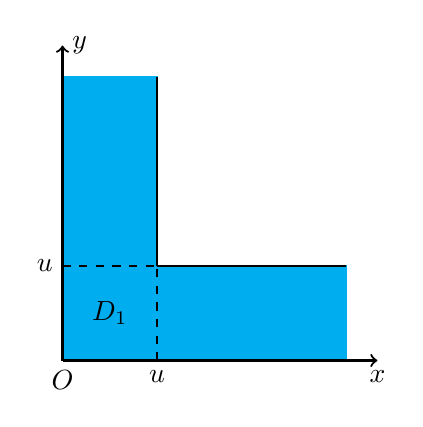
\begin{tikzpicture}[scale=.4]
            \draw [cyan,fill=cyan] (0,0) -- (9,0) -- (9,3) -- (3,3) -- (3,9) -- (0,9) -- (0,0);
            \draw [thick,->] (0,0) -- (10,0);
            \draw [thick,->] (0,0) -- (0,10);
            \draw [thick,dashed] (3,0) -- (3,3);
            \draw [thick,dashed] (0,3) -- (3,3);
            \draw [thick] (3,3) -- (3,9);
            \draw [thick] (3,3) -- (9,3);
            \node [below] at (0,0) {$O$};
            \node at (1.5,1.5) {$D_1$};
            \node [below] at (10,0) {$x$};
            \node [right] at (0,10) {$y$};
            \node [left] at (0,3) {$u$};
            \node [below] at (3,0) {$u$};
        \end{tikzpicture}
        \quad\quad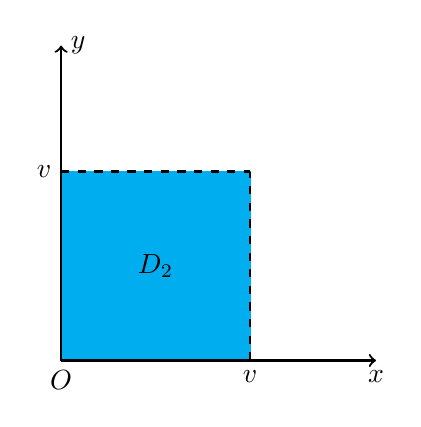
\begin{tikzpicture}[scale=.4]
            \draw [cyan,fill=cyan] (0,0) -- (6,0) -- (6,6) -- (0,6) -- (0,0);
            \draw [thick,->] (0,0) -- (10,0);
            \draw [thick,->] (0,0) -- (0,10);
            \draw [thick,dashed] (6,0) -- (6,6);
            \draw [thick,dashed] (0,6) -- (6,6);
            \node at (3,3) {$D_2$};
            \node [below] at (0,0) {$O$};
            \node [below] at (10,0) {$x$};
            \node [right] at (0,10) {$y$};
            \node [left] at (0,6) {$v$};
            \node [below] at (6,0) {$v$};
        \end{tikzpicture}
        \caption{左图为 $D_1=\{\min(X,Y)\leq u\}$, 右图为 $D_2=\{\max(X,Y)\leq v\}$}\label{f8.1}
    \end{figure}
\end{note}
\begin{exercise}% 4.31
    设随机向量 $(X,Y)$ 有联合密度 $f(x)g(y)$, $(U,V)$ 有联合密度
    \[p(u,v)=\begin{cases}
        \dfrac{1}{\alpha}f(u)g(v), & u\geq v, \\[6pt]
        0 & u<v,
    \end{cases}\]

    (a) 求 $U,V$ 的边缘密度;

    (b) 证明 $\alpha=P(X\geq Y)$.
\end{exercise}
\begin{proof}
    (a) $\because$
    \begin{align*}
        P(U\leq u) & =\iint\limits_{x\leq u}\dfrac{1}{\alpha}f(x)g(y)I[x<y]\mathrm{d}x\mathrm{d}y \\
        & =\int_{-\infty}^u\dfrac{1}{\alpha}f(x)\mathrm{d}x\int_{-\infty}^xg(y)\mathrm{d}y \\
        & =\int_{-\infty}^u\dfrac{1}{\alpha}f(x)G(x)\mathrm{d}x,
    \end{align*}

    其中 $G(x)=\int_{-\infty}^xg(y)\mathrm{d}y$, $\therefore U$ 的概率密度为 $f_U(u)=\dfrac{1}{\alpha}f(x)G(x)$. $\because$
    \begin{align*}
        P(V\leq v) & =1-P(V>v) \\
        & =1-\iint\limits_{y>v}\dfrac{1}{\alpha}f(x)g(y)I[x<y]\mathrm{d}x\mathrm{d}y \\
        & =1-\int_v^\infty\dfrac{1}{\alpha}g(y)\mathrm{d}y\int_y^\infty f(x)\mathrm{d}x \\
        & =1-\int_v^\infty\dfrac{1}{\alpha}g(y)F(y)\mathrm{d}y,
    \end{align*}

    其中 $F(y)=\int_{-\infty}^yf(x)\mathrm{d}x$, $\therefore U$ 的概率密度为 $f_V(v)=\dfrac{1}{\alpha}g(y)F(y)$.

    (b) 有
    \begin{align*}
        P(X\geq Y) & =\iint\limits_{x>y}f(x)g(y)\mathrm{d}x\mathrm{d}y \\
        & =\alpha\int_{-\infty}^\infty\dfrac{1}{\alpha}f(x)\mathrm{d}x\int_{-\infty}^xg(y)\mathrm{d}y \\
        & =\alpha\cdot P(U\leq\infty)=\alpha.\qedhere
    \end{align*}
\end{proof}
\begin{exercise}% 4.32
    随机变量 $X,Y$ 相互独立, $X$ 有分布函数 $F_X(x)$ 和概率密度 $f_X(x)=F_X'(x)$. 如果 $P(Y>y)=(P(X>y))^\beta$, 其中 $\beta$ 是正常数, 求 $P(X\geq Y)$.
\end{exercise}
\begin{solution}
    $Y$ 的分布函数为
    \[F_Y(y)=1-P(Y>y)=1-(P(X>y))^\beta=1-(1-F_X(x))^\beta.\]

    $\because X$ 有概率密度 $f_X(x)$, $\therefore F_X(x)$ 可导. $\therefore F_Y(y)$ 可导. $\therefore Y$ 有概率密度 $f_Y(y)=F'_Y(y)$. 有
    \begin{align*}
        P(X\geq Y) & =\iint\limits_{x\geq y}f_X(x)f_Y(y)\mathrm{d}x\mathrm{d}y \\
        & =\int_{-\infty}^\infty f_X(x)\mathrm{d}x\int_{-\infty}^x f_Y(y)\mathrm{d}y \\
        & =\int_{-\infty}^\infty f_X(x)F_Y(x)\mathrm{d}x \\
        & =\int_{-\infty}^\infty F'_X(x)(1-(1-F_X(x))^\beta)\mathrm{d}x.
    \end{align*}

    令 $t=F_X(x)$, 则 $x=\infty$ 时 $t=1$, $x=-\infty$ 时 $t=0$. 有
    \[\int_{-\infty}^\infty F'_X(x)(1-(1-F_X(x))^\beta)\mathrm{d}x=\int_0^1(1-(1-t)^\beta)\mathrm{d}t=\dfrac{\beta}{1+\beta}.\]
\end{solution}
\begin{exercise}[有修改]\label{ex4.36}
    证明: 如果 $\mathbb{R}^2$ 上的随机向量 $(X,Y)$ 有联合密度 $f(x,y)$, $(U,V)$ 由线性变换
    \[\begin{pmatrix}
        U \\ V
    \end{pmatrix}=\boldsymbol{A}\begin{pmatrix}
        X \\ Y
    \end{pmatrix}+\begin{pmatrix}
        \mu_1 \\ \mu_2
    \end{pmatrix}\]
    决定, 其中
    \[\boldsymbol{A}=\begin{pmatrix}
        a & b \\
        c & d \\
    \end{pmatrix},\quad\boldsymbol{A}^{-1}=\begin{pmatrix}
        a_1 & b_1 \\
        c_1 & d_1 \\
    \end{pmatrix},\]

    则 $(U,V)$ 有联合密度
    \[g(u,v)=\dfrac{1}{|\det\boldsymbol{A}|}f((u-\mu_1,v-\mu_2)\boldsymbol{A}^{-T}),\quad(u,v)\in\mathbb{R}^2,\]

    其中 $\boldsymbol{A}^{-T}=(A^{-1})^T$.
\end{exercise}
\begin{proof}
    $\forall u,v$, 有
    \begin{align*}
        P(U=u,V=v) & =P\left(\boldsymbol{A}\begin{pmatrix}
            X \\ Y
        \end{pmatrix}+\begin{pmatrix}
            \mu_1 \\ \mu_2
        \end{pmatrix}=\begin{pmatrix}
            u \\ v
        \end{pmatrix}\right) \\
        & =P\left(\begin{pmatrix}
            X \\ Y
        \end{pmatrix}=\boldsymbol{A}^{-1}\begin{pmatrix}
            u-\mu_1 \\ v-\mu_2
        \end{pmatrix}\right).
    \end{align*}

    $\because\dfrac{\partial(x,y)}{\partial(u,v)}=|\boldsymbol{A}^{-1}|$, $\therefore$ 
    \begin{align*}
        P\left(\begin{pmatrix}
            X \\ Y
        \end{pmatrix}=\boldsymbol{A}^{-1}\begin{pmatrix}
            u-\mu_1 \\ v-\mu_2
        \end{pmatrix}\right) & =f\left(\left(\boldsymbol{A}^{-1}\begin{pmatrix}
            u-\mu_1 \\ v-\mu_2
        \end{pmatrix}\right)^T\right)|\det\boldsymbol{A}^{-1}|\mathrm{d}u\mathrm{d}v \\
        & =f((u-\mu_1,v-\mu_2)\boldsymbol{A}^{-T})|\det\boldsymbol{A}^{-1}|\mathrm{d}u\mathrm{d}v \\
        & =\dfrac{1}{|\det\boldsymbol{A}|}f((u-\mu_1,v-\mu_2)\boldsymbol{A}^{-T})\mathrm{d}u\mathrm{d}v.
    \end{align*}

    $\therefore$
    \[g(u,v)=\dfrac{1}{|\det\boldsymbol{A}|}f((u-\mu_1,v-\mu_2)\boldsymbol{A}^{-T}).\qedhere\]
\end{proof}
\section{第5章笔记}
可以证明, 任意的概率空间 $(\Omega,\mathcal{F},P)$ 上所有有二阶矩的随机变量构成的线性空间(其中的加法和纯量乘法是随机变量的加法和纯量乘法)是一个 Hilbert 空间, 内积为 $\left<X,Y\right>=E(XY)$. 这个 Hilbert 空间是无穷维的. 第 7 章第 6 节介绍的均方收敛可以看成是在这个 Hilbert 空间中收敛.

书上的例 4.5 用到了下面的引理.
\begin{lemma}
    设 $X$ 是随机变量, 如果 $\int_0^\infty P(|X|>x)\mathrm{d}x=0$, 那么 $\forall x>0,P(|X|>x)=0$.
\end{lemma}
\begin{proof}
    假设 $\exists x_0>0$ 使得 $P(|X|>x_0)=\varepsilon>0$, 则 $\forall x\in(0,x_0),P(|X|>x)\geq P(|X|>x_0)=\varepsilon$. $\therefore$
    \[\int_0^\infty P(|X|>x)\mathrm{d}x\geq\int_0^{x_0}P(|X|>x)\mathrm{d}x\geq x_0\varepsilon>0.\]

    这与 $\int_0^\infty P(|X|>x)\mathrm{d}x=0$ 矛盾.
\end{proof}

补充几个定理的证明.
\begin{theorem}[书上的定理 5.2]\label{t9.1}
    设 $a,b,c$ 是常数, $\mu_j=EX_j,\operatorname{Var}(X_j)<\infty\ (1\leq j\leq n)$, 则
    
    (4) $\operatorname{Var}\left(\sum\limits_{j=1}^nX_j\right)=\sum\limits_{i=1}^n\sum\limits_{j=1}^n(E(X_iX_j)-\mu_i\mu_j)$;
    
    (5) 当 $X_1,X_2,\cdots,X_n$ 相互独立时, $\operatorname{Var}\left(\sum\limits_{j=1}^nX_j\right)=\sum\limits_{j=1}^n\operatorname{Var}(X_j)$.
\end{theorem}
\begin{proof}
    (4) 有
    \begin{align*}
        \operatorname{Var}\left(\sum\limits_{j=1}^nX_j\right) & =E\left(\sum\limits_{j=1}^nX_j-\sum\limits_{j=1}^n\mu_j\right)^2 \\
        & =E\left(\left(\sum\limits_{j=1}^nX_j\right)^2+\left(\sum\limits_{j=1}^n\mu_j\right)^2-2\left(\sum\limits_{j=1}^nX_j\right)\left(\sum\limits_{j=1}^n\mu_j\right)\right) \\
        & =E\left(\left(\sum\limits_{j=1}^nX_j\right)^2-\left(\sum\limits_{j=1}^n\mu_j\right)^2-2\left(\sum\limits_{j=1}^nX_j-\sum\limits_{j=1}^n\mu_j\right)\left(\sum\limits_{j=1}^n\mu_j\right)\right) \\
        & =E\left(\sum\limits_{j=1}^nX_j\right)^2-\left(\sum\limits_{j=1}^n\mu_j\right)^2-E\left(2\left(\sum\limits_{j=1}^nX_j-\sum\limits_{j=1}^n\mu_j\right)\left(\sum\limits_{j=1}^n\mu_j\right)\right) \\
        & =E\left(\sum\limits_{i=1}^n\sum\limits_{j=1}^nX_iX_j\right)-\left(\sum\limits_{i=1}^n\sum\limits_{j=1}^n\mu_i\mu_j\right)-2\left(\sum\limits_{j=1}^n\mu_j\right)\left(\sum\limits_{j=1}^nEX_j-\sum\limits_{j=1}^n\mu_j\right) \\
        & =\left(\sum\limits_{i=1}^n\sum\limits_{j=1}^nE(X_iX_j)\right)-\left(\sum\limits_{i=1}^n\sum\limits_{j=1}^n\mu_i\mu_j\right)-2\left(\sum\limits_{j=1}^n\mu_j\right)\sum\limits_{j=1}^n(EX_j-\mu_j) \\
        & =\sum\limits_{i=1}^n\sum\limits_{j=1}^n(E(X_iX_j)-\mu_i\mu_j).
    \end{align*}

    (5) $\because X_1,X_2,\cdots,X_n$ 相互独立, $\therefore\forall i,j=1,2,\cdots,n,j\neq i,E(X_iX_j)=EX_iEX_j$. 由 (4) 得
    \begin{align*}
        \operatorname{Var}\left(\sum\limits_{j=1}^nX_j\right) & =\sum\limits_{i=1}^n\sum\limits_{j=1}^n(E(X_iX_j)-\mu_i\mu_j) \\
        & =\sum\limits_{i=1}^n\sum\limits_{\substack{j=1\\j\neq i}}^n(EX_iEX_j-\mu_i\mu_j)+\sum\limits_{i=1}^n(EX_i^2-\mu_i^2) \\
        & =\sum\limits_{i=1}^n(EX_i^2-(EX_i)^2)=\sum\limits_{i=1}^n\operatorname{Var}(X_i).
    \end{align*}
\end{proof}
\begin{theorem}[书上的定理 6.2]
    设 $\rho_{XY}$ 是 $X,Y$ 的相关系数, 则有
    
    (1) $|\rho_{XY}|\leq 1$;

    (2) $|\rho_{XY}|=1$ 的充要条件为有常数 $a,b$ 使得 $P(Y=a+bX)=1$;

    (3) 如果 $X,Y$ 独立, 则 $X,Y$ 不相关.
\end{theorem}
\begin{proof}
    (1) 由定义,
    \[|\rho_{XY}|=\dfrac{|E((X-\mu_X)(Y-\mu_Y))|}{\sigma_X\sigma_Y}.\]

    由内积不等式(书上的定理 6.1),
    \begin{equation}\label{eq9.1}
        |E((X-\mu_X)(Y-\mu_Y))|\leq\sqrt{E(X-\mu_X)^2E(Y-\mu_Y)^2}=\sigma_X\sigma_Y,
    \end{equation}

    $\therefore|\rho_{XY}|\leq 1$.

    (2) 由内积不等式取等号的充要条件得式 (\ref{eq9.1}) 成立的充要条件是有常数 $a,b$ 使得 $P(Y-\mu_Y=a+b(X-\mu_X))=1$, 即有常数 $b,a'=a+\mu_Y-b\mu_X$ 使得 $P(Y=a'+bX)$.

    (3) $\because X,Y$ 独立, $\therefore$ 由书上的定理 4.1 得 $E(XY)=EXEY$. 由书上的式 (6.6) 得
    \[\sigma_{XY}=E(XY)-EXEY=0.\qedhere\]
\end{proof}

设随机向量 $(X,Y)$ 服从二维 Gauss 分布, 则分布由 $X$ 的均值 $\mu_X$, 方差 $\sigma_X$, $Y$ 的均值 $\mu_Y$, 方差 $\sigma_Y$, $X,Y$ 的相关系数 $\rho_{XY}$ 这 $5$ 个量完全确定. $\therefore$ 可以用 $(X,Y)\sim N(\mu_X,\mu_Y;\sigma_X,\sigma_Y;\rho_{XY})$ 来表示 $(X,Y)$ 服从由这 $5$ 个量确定的二维 Gauss 分布.
\section{第5章习题}
\addtocounter{exsection}{5}
\addtocounter{exercise}{4}
\begin{exercise}% 5.5
    一部手机收到的短信中有 $p=2\%$ 是广告, 你期望相邻的两次广告短信中有多少个不是广告短信?
\end{exercise}
\begin{solution}
    设 $X$ 为相邻的两次广告短信中不是广告短信的数目, 则 $P(X=k)=p^k(1-p)$. 有
    \begin{align*}
        EX & =\sum\limits_{k=0}^\infty kP(X=k) \\
        & =\sum\limits_{k=1}^\infty kp^k(1-p) \\
        & =p(1-p)\sum\limits_{k=1}^\infty kp^{k-1} \\
        & =p(1-p)\left(\sum\limits_{k=1}^\infty\dfrac{\partial}{\partial x}x^k\right)\Bigg|_{x=p} \\
        & =p(1-p)\left(\dfrac{\partial}{\partial x}\sum\limits_{k=0}^\infty x^k\right)\Bigg|_{x=p} \\
        & =p(1-p)\left(\dfrac{\partial}{\partial x}\dfrac{1}{1-x}\right)\Bigg|_{x=p} \\
        & =p(1-p)\cdot\dfrac{1}{(1-p)^2}=\dfrac{p}{1-p}.
    \end{align*}

    把 $p=2\%$ 代入得 $EX=49$.
\end{solution}
\addtocounter{exercise}{2}
\begin{exercise}% 5.8
    设 $X,Y$ 独立, 都服从 Gauss 分布, 求 $R=\sqrt{X^2+Y^2}$ 的数学期望.
\end{exercise}
\begin{solution}
    由书上的定理 4.3 得 $R$ 有 Rayleigh 概率密度
    \[f_R(r)=re^{-r^2/2}.\]

    $\therefore$
    \begin{align*}
        ER & =\int_{-\infty}^\infty r^2e^{-r^2/2}\mathrm{d}r \\
        & =\int_{-\infty}^\infty re^{-r^2/2}\mathrm{d}r^2/2 \\
        & =\sqrt{2}\int_0^\infty t^{1/2}e^{-t}\mathrm{d}t \\
        & =\sqrt{2}\Gamma(3/2)=\sqrt{\dfrac{\pi}{2}}.
    \end{align*}
\end{solution}
\begin{exercise}% 5.9
    设 $X_1,X_2,\cdots,X_n$ 独立同分布, 且 $P(X_i>0)=1$. 对于 $k\leq n$, 计算
    \[E\dfrac{X_1+X_2+\cdots+X_k}{X_1+X_2+\cdots+X_n}.\]
\end{exercise}
\begin{solution}
    设
    \[Y_i=\dfrac{X_i}{X_1+X_2+\cdots+X_n},\quad (n=1,2,\cdots,n).\]
    
    $\because X_1,X_2,\cdots,X_n$ 独立同分布, $\therefore Y_1,Y_2,\cdots,Y_n$ 同分布. $\because P(X_i>0)=1,\therefore P(Y_i>0)=1$. 有
    \[1=E\dfrac{X_1+X_2+\cdots+X_n}{X_1+X_2+\cdots+X_n}=EY_1+EY_2+\cdots+EY_n=nEY_1,\]
    \[E\dfrac{X_1+X_2+\cdots+X_k}{X_1+X_2+\cdots+X_n}=EY_1+EY_2+\cdots+EY_k=kEY_1,\]

    $\therefore$
    \[E\dfrac{X_1+X_2+\cdots+X_k}{X_1+X_2+\cdots+X_n}=\dfrac{k}{n}.\]
\end{solution}
\addtocounter{exercise}{2}
\begin{exercise}% 5.12
    设 $X_1,X_2,\cdots,X_n$ 相互独立, 有共同的离散分布 $p_k=P(X=k),\ k=1,2,\cdots$. 引入 $u_k=p_1+p_2+\cdots+p_{k-1},v_k=1-u_k$, 证明:
    \[E[\min(X_1,X_2,\cdots,X_n)]=\sum\limits_{k=1}^\infty v_k^n,\quad E[\max(X_1,X_2,\cdots,X_n)]=\sum\limits_{k=1}^\infty(1-u_k^n).\]
\end{exercise}
\begin{proof}
    由书上的定理 3.2 (3) 得
    \begin{align*}
        E[\min(X_1,X_2,\cdots,X_n)] & =\sum\limits_{k=1}^\infty P(\min(X_1,X_2,\cdots,X_n)\geq k) \\
        & =\sum\limits_{k=1}^\infty P(X_1\geq k,X_2\geq k,\cdots,X_n\geq k) \\
        & =\sum\limits_{k=1}^\infty P(X_1\geq k)P(X_2\geq k)\cdots P(X_n\geq k) \\
        & =\sum\limits_{k=1}^\infty (1-P(X_1\geq k))(1-P(X_2\geq k))\cdots(1-P(X_n\geq k)) \\
        & =\sum\limits_{k=1}^\infty v_k^n,
    \end{align*}
    \begin{align*}
        E[\max(X_1,X_2,\cdots,X_n)] & =\sum\limits_{k=1}^\infty P(\max(X_1,X_2,\cdots,X_n)\geq k) \\
        & =\sum\limits_{k=1}^\infty1-P(\max(X_1,X_2,\cdots,X_n)<k) \\
        & =\sum\limits_{k=1}^\infty1-P(X_1<k,X_2<k,\cdots,X_n<k) \\
        & =\sum\limits_{k=1}^\infty1-P(X_1<k)P(X_2<k)\cdots P(X_n<k) \\
        & =\sum\limits_{k=1}^\infty1-u_k^n.\qedhere
    \end{align*}
\end{proof}
\stepcounter{exercise}
\begin{exercise}[1]% 5.14
    设 $(X,Y)$ 有概率密度
    \[f(x,y)=\begin{cases}
        \dfrac{3}{2x^2y^3}, & x>1,1<xy<x^2, \\[6pt]
        0, & \text{otherwise}.
    \end{cases}\]

    计算 $EY$.
\end{exercise}
\begin{solution}
    有 $1<xy<x^2\Rightarrow\dfrac{1}{x}<y<x$. 由书上的定理 3.1 (2),
    \begin{align*}
        EY & =\iint_{\mathbb{R}^2}yf(x,y)\mathrm{d}x\mathrm{d}y \\
        & =\int_1^\infty\mathrm{d}x\int_{1/x}^xy\dfrac{3}{2x^3y^2}\mathrm{d}y \\
        & =\int_1^\infty\dfrac{3}{2x^3}\mathrm{d}x\int_{1/x}^x\dfrac{1}{y}\mathrm{d}y \\
        & =\int_1^\infty\dfrac{3(\ln x-\ln (1/x))}{2x^3}\mathrm{d}x \\
        & =\int_1^\infty\dfrac{3\ln x}{x^2}\mathrm{d}\ln x \\
        & =\int_0^\infty3te^{-2t}\mathrm{d}t=\dfrac{3}{4}.
    \end{align*}
\end{solution}
\addtocounter{exercise}{2}
\begin{exercise}[b]% 5.17
    设 $5$ 台计算机独立工作, 每台计算机感染病毒前的时间(分别记作 $X_1,\cdots,X_5$)都服从参数为 $\lambda$ 的指数分布 $\mathcal{E}(\lambda)$. 对 $5$ 台计算机都感染病毒前的时间的数学期望是多少?
\end{exercise}
\begin{solution}
    记 $Y=\max(X_1,\cdots,X_5)$, 则
    \begin{align*}
        P(Y>y) & =1-P(Y\leq y) \\
        & =1-P(X_1\leq y,X_2\leq y,\cdots,X_5\leq y) \\
        & =1-P(X_1\leq y)P(X_2\leq y)\cdots P(X_5\leq y) \\
        & =1-(1-e^{-\lambda y})^5 \\
        & =1-\left(1+\sum\limits_{i=1}^5C_5^i(-e^{-\lambda y})^i\right) \\
        & =\sum\limits_{i=1}^5C_5^i(-1)^{i-1}e^{-\lambda iy}.
    \end{align*}

    由书上的定理 3.1 (3) 得
    \begin{align*}
        EY & =\int_0^\infty P(Y>y)\mathrm{d}y \\
        & =\int_0^\infty\sum\limits_{i=1}^5C_5^i(-1)^{i-1}e^{-\lambda iy}\mathrm{d}y \\
        & =\sum\limits_{i=1}^5C_5^i(-1)^{i-1}\int_0^\infty e^{-\lambda iy}\mathrm{d}y \\
        & =\sum\limits_{i=1}^5C_5^i\dfrac{1}{\lambda i}(-1)^{i-1}=\dfrac{137}{60\lambda}.
    \end{align*}
\end{solution}
\addtocounter{exercise}{2}
\begin{exercise}% 5.20
    设 $n\geq 2$, $X_1,X_2,\cdots,X_n$ 独立同分布,
    \[\hat{\mu}=\dfrac{1}{n}\sum\limits_{j=1}^nX_j,\quad\hat{\sigma}^2=\dfrac{1}{n-1}\sum\limits_{j=1}^n(X_j-\hat{\mu})^2,\]

    验证 $E\hat{\mu}=EX_1,E\hat{\sigma}^2=\operatorname{Var}(X_1)$.
\end{exercise}
\begin{proof}
    $\because X_1,X_2,\cdots,X_n$ 独立同分布, $\therefore$
    \[E\hat{\mu}=\dfrac{1}{n}\sum\limits_{j=1}^nEX_j=\dfrac{1}{n}\sum\limits_{j=1}^nEX_1=EX_1.\]

    $\therefore$
    \begin{align*}
        E\hat{\sigma}^2 & =\dfrac{1}{n-1}\sum\limits_{j=1}^nE(X_j-\hat{\mu})^2 \\
        & =\dfrac{1}{n-1}\sum\limits_{j=1}^nE\left(X_j-\dfrac{1}{n}\sum\limits_{i=1}^nX_i\right)^2 \\
        & =\dfrac{1}{n-1}\sum\limits_{j=1}^nE\left(\dfrac{n-1}{n}X_j-\dfrac{1}{n}\sum\limits_{\substack{i=1\\i\neq j}}^nX_i\right)^2 \\
        & =\dfrac{1}{n-1}\sum\limits_{j=1}^nE\left(\dfrac{n-1}{n}(X_j-EX_1)-\dfrac{1}{n}\sum\limits_{\substack{i=1\\i\neq j}}^n(X_i-EX_1)\right)^2.
    \end{align*}

    令 $Y_i=X_i-EX_1\ (i=1,2,\cdots,n)$, 则 $Y_i$ 独立同分布, 均值为 $0$, 方差为 $\operatorname{Var}(X_1)$. $\therefore\forall i=1,\cdots,n,j=1,\cdots,\hat{i},\cdots,n,E(X_iX_j)=E(X_i)E(X_j)=0$. 有
    \begin{align*}
        E\hat{\sigma}^2 & =\dfrac{1}{n-1}\sum\limits_{j=1}^nE\left(\dfrac{n-1}{n}Y_j-\dfrac{1}{n}\sum\limits_{\substack{i=1\\i\neq j}}^nY_i\right)^2 \\
        & =\dfrac{1}{n-1}\sum\limits_{j=1}^nE\left(\left(\dfrac{n-1}{n}Y_j\right)^2+\left(\dfrac{1}{n}\sum\limits_{\substack{i=1\\i\neq j}}^nY_i\right)^2-2\dfrac{n-1}{n}Y_j\left(\dfrac{1}{n}\sum\limits_{\substack{i=1\\i\neq j}}^nY_i\right)\right) \\
        & =\dfrac{1}{n-1}\sum\limits_{j=1}^n\left(\left(\dfrac{n-1}{n}\right)^2EY_j^2+\dfrac{1}{n^2}\sum\limits_{\substack{i=1\\i\neq j}}^n\sum\limits_{\substack{k=1\\k\neq j}}^nE(Y_iY_k)-2\dfrac{n-1}{n^2}\sum\limits_{\substack{i=1\\i\neq j}}^nE(Y_iY_j)\right) \\
        & =\dfrac{1}{n-1}\sum\limits_{j=1}^n\left(\left(\dfrac{n-1}{n}\right)^2EY_j^2+\dfrac{1}{n^2}\sum\limits_{\substack{i=1\\i\neq j}}^nEY_i^2+\dfrac{1}{n^2}\sum\limits_{\substack{i=1\\i\neq j}}^n\sum\limits_{\substack{k=1\\k\neq j\\k\neq i}}^nE(Y_iY_k)-2\dfrac{n-1}{n^2}\sum\limits_{\substack{i=1\\i\neq j}}^nE(Y_iY_j)\right) \\
        & =\dfrac{1}{n-1}\sum\limits_{j=1}^n\left(\left(\dfrac{n-1}{n}\right)^2E(Y_j-EY_j)^2+\dfrac{1}{n^2}\sum\limits_{\substack{i=1\\i\neq j}}^nE(Y_i-EY_i)^2\right) \\
        & =\dfrac{1}{n-1}\sum\limits_{j=1}^n\left(\left(\dfrac{n-1}{n}\right)^2\operatorname{Var}(X_1)+\dfrac{1}{n^2}\sum\limits_{\substack{i=1\\i\neq j}}^n\operatorname{Var}(X_1)\right) \\
        & =\dfrac{1}{n-1}\sum\limits_{j=1}^n\left(\dfrac{(n-1)^2}{n^2}\operatorname{Var}(X_1)+\dfrac{n-1}{n^2}\operatorname{Var}(X_1)\right) \\
        & =\sum\limits_{j=1}^n\dfrac{1}{n}\operatorname{Var}(X_1)=\operatorname{Var}(X_1).\qedhere
    \end{align*}
\end{proof}
\stepcounter{exercise}
\begin{exercise}% 5.22
    设 $X_1,X_2,\cdots,X_n$ 是相互独立的随机变量, $\operatorname{Var}(X_i)=\sigma_i^2$. 求满足 $\sum\limits_{j=1}^na_j=1,a_j\geq0$ 的常数 $a_1,a_2,\cdots,a_n$ 使得 $Y=\sum\limits_{j=1}^na_jX_j$ 的方差最小.
\end{exercise}
\begin{solution}
    $\because X_1,X_2,\cdots,X_n$ 相互独立, $\therefore$
    \begin{align*}
        P(a_1X_1\leq x_1,a_2X_2\leq x_2,\cdots,a_nX_n\leq x_n) & =P(X_1\leq x_1/a_1,X_2\leq x_2/a_2,\cdots,X_n\leq x_n/a_n) \\
        & =P(X_1\leq x_1/a_1)P(X_2\leq x_2/a_2)\cdots P(X_n\leq x_n/a_n) \\
        & =P(a_1X_1\leq x_1)P(a_2X_2\leq x_2)\cdots P(a_nX_n\leq x_n).
    \end{align*}

    $\therefore a_1X_1,a_2X_2,\cdots,a_nX_n$ 相互独立. 由定理 \ref{t9.1} (5) 得
    \[\operatorname{Var}(Y)=\sum\limits_{j=1}^n\operatorname{Var}(a_jX_j)=\sum\limits_{j=1}^na_j^2\sigma_i^2.\]

    由 Cauchy 不等式得
    \[1=\sum\limits_{j=1}^na_j\sigma_j\cdot\dfrac{1}{\sigma_j}\leq\left(\sum\limits_{j=1}^n(a_j\sigma_i)^2\right)\left(\sum\limits_{j=1}^n\dfrac{1}{\sigma_j^2}\right),\]

    当且仅当 $a_j\sigma_j=\lambda\cdot\dfrac{1}{\sigma_j},\ j=1,2,\cdots,n$ 时取等号. $\therefore a_j=\dfrac{\sigma_j^{-2}}{\sum\limits_{i=1}^n\sigma_i^{-2}},\ j=1,2,\cdots,n$.
\end{solution}
\addtocounter{exercise}{2}
\begin{exercise}% 5.25
    设非负随机变量 $X$ 有离散分布 $p_j=P(X=x_j),j\geq 1$. 证明:
    
    (1) $P(X>x)=\sum\limits_{j=1}^\infty p_jI[x<x_j]$;

    (2) $EX=\int_0^\infty P(X>x)\mathrm{d}x$.
\end{exercise}
\begin{proof}
    (1) 有 $\forall j,P(X>x|X=x_j)=I[x<x_j]$. 由全概率公式得
    \[P(X>x)=\sum\limits_{j=1}^\infty P(X>x|X=x_j)P(X=x_j)=\sum\limits_{j=1}^\infty p_jI[x<x_j].\]

    (2) 由 (1) 得
    \[\int_0^\infty P(X>x)\mathrm{d}x=\int_0^\infty\sum\limits_{j=1}^\infty p_jI[x<x_j]\mathrm{d}x.\]

    $\because\sum\limits_{j=1}^\infty p_jI[x<x_j]\leq\sum\limits_{j=1}^\infty p_j=1$, 由 Weierstrass 判别法得 $\sum\limits_{j=1}^\infty p_jI[x<x_j]$ 在 $(0,\infty)$ 上一致收敛, $\therefore$ 求和号和积分号可以交换次序. 有
    \begin{align*}
        \int_0^\infty\sum\limits_{j=1}^\infty p_jI[x<x_j]\mathrm{d}x & =\sum\limits_{j=1}^\infty p_j\int_0^\infty I[x<x_j]\mathrm{d}x \\
        & =\sum\limits_{j=1}^\infty p_j\int_0^{x_j}\mathrm{d}x \\
        & =\sum\limits_{j=1}^\infty p_jx_j=EX.\qedhere
    \end{align*}
\end{proof}
\begin{exercise}% 5.26
    如果 $\operatorname{Cov}(X,Y)=0$, 验证 $\rho(X+Y,X-Y)=\dfrac{\operatorname{Var}(X)-\operatorname{Var}(Y)}{\operatorname{Var}(X)+\operatorname{Var}(Y)}$.
\end{exercise}
\begin{proof}
    定义 $E^2X:=(EX)^2$. 由书上的式 (6.6) 得
    \begin{align*}
        \operatorname{Cov}(X+Y,X-Y) & =E((X+Y)(X-Y))-E(X+Y)E(X-Y) \\
        & =E(X^2-Y^2)-(EX+EY)(EX-EY) \\
        & =EX^2-EY^2-(E^2X-E^2Y) \\
        & =(EX^2-E^2X)-(EY^2-E^2Y) \\
        & =\operatorname{Var}(X)-\operatorname{Var}(Y).
    \end{align*}

    由书上的式 (5.2) 得
    \begin{align*}
        \operatorname{Var}(X\pm Y) & =E(X\pm Y)^2-E^2(X\pm Y) \\
        & =E(X^2+Y^2\pm2XY)-(EX\pm EY)^2 \\
        & =EX^2+EY^2\pm2E(XY)-(E^2X+E^2Y\pm2EXEY) \\
        & =(EX^2-E^2X)+(EY^2-E^2Y)\pm2(E(XY)-EXEY) \\
        & =\operatorname{Var}(X)+\operatorname{Var}(Y)\pm2\operatorname{Cov}(X,Y).
    \end{align*}

    $\because\operatorname{Cov}(X,Y)=0$, $\therefore\operatorname{Var}(X\pm Y)=\operatorname{Var}(X)+\operatorname{Var}(Y)$,
    \begin{align*}
        \rho(X+Y,X-Y) & =\dfrac{\operatorname{Cov}(X+Y,X-Y)}{\sqrt{\operatorname{Var}(X+Y)\operatorname{Var}(X-Y)}} \\
        & =\dfrac{\operatorname{Var}(X)-\operatorname{Var}(Y)}{\sqrt{(\operatorname{Var}(X)+\operatorname{Var}(Y))^2}} \\
        & =\dfrac{\operatorname{Var}(X)-\operatorname{Var}(Y)}{\operatorname{Var}(X)+\operatorname{Var}(Y)}.\qedhere
    \end{align*}
\end{proof}
\stepcounter{exercise}
\begin{exercise}% 5.28
    设 $(X,Y)$ 有概率密度
    \[f(x,y)=\begin{cases}
        x+y & x\in(0,1),y\in(0,1), \\
        0 & \text{otherwise}.
    \end{cases}\]

    计算 $\operatorname{Cov}(X,Y)$.
\end{exercise}
\begin{solution}
    有
    \[f_X(x)=\int_{-\infty}^\infty f(x,y)\mathrm{d}y=\int_0^1(x+y)\mathrm{d}y=x+\dfrac{1}{2},\quad x\in(0,1),\]
    \[EX=\int_{-\infty}^\infty xf_X(x)\mathrm{d}x=\dfrac{7}{12}.\]

    对称地, 有 $EY=\dfrac{7}{12}$.

    \[E(XY)=\iint_{\mathbb{R}^2}xyf(x,y)\mathrm{d}x\mathrm{d}y=\int_0^1\mathrm{d}x\int_0^1xy(x+y)\mathrm{d}y=\dfrac{1}{3}.\]

    $\therefore$
    \[\operatorname{Cov}(X,Y)=E(XY)-EXEY=-\dfrac{1}{144}.\]
\end{solution}
\stepcounter{exercise}
\begin{exercise}% 5.30
    设活塞的直径 $X$ 的平均值为 $20.00\text{cm}$, 标准差为 $0.02$; 气缸的直径 $Y$ 的平均值为 $20.10\text{cm}$, 标准差为 $0.02$. 设 $X$ 与 $Y$ 独立且都服从 Gauss 分布, 计算活塞能装入气缸的概率.
\end{exercise}
\begin{solution}
    事件 ``活塞能装入气缸'' 等价于事件 $A=\{X<Y\}$. 设 $(X,Y)$ 的联合密度为 $f(x,y)$, 则
    \[P(A)=\iint_{\mathbb{R}^2}f(x,y)I[x<y]\mathrm{d}x\mathrm{d}y=\iint\limits_{x<y}f(x,y)\mathrm{d}x\mathrm{d}y.\]

    由题得
    \[f(x,y)=\dfrac{1}{2\pi\cdot0.02^2}\exp\left(-\dfrac{(x-20.0)^2}{2\cdot0.02^2}-\dfrac{(y-20.1)^2}{2\cdot0.02^2}\right).\]

    $\therefore$
    \[P(A)=\int_{-\infty}^\infty\mathrm{d}y\int_{-\infty}^y\dfrac{1}{2\pi\cdot0.02^2}\exp\left(-\dfrac{(x-20.0)^2}{2\cdot0.02^2}-\dfrac{(y-20.1)^2}{2\cdot0.02^2}\right)\mathrm{d}x\approx0.9998.\]
\end{solution}
\begin{note}
    我不会算这个积分, 所以用了 Mathematica 的数值积分来计算. 理论上, 对 $\forall a$
    \[\int_{-\infty}^\infty\mathrm{d}y\int_{-\infty}^y\dfrac{1}{2\pi\cdot0.02^2}\exp\left(-\dfrac{(x-a)^2}{2\cdot0.02^2}-\dfrac{(y-a-0.1)^2}{2\cdot0.02^2}\right)\mathrm{d}x\]
    的值都一样, 都为 $P(A)$, 但是在 Mathematica 中, 上式取不同的 $a$, 计算结果不一样.

    取 $a=-10,0,10,20$ 分别计算上式的 Mathematica 程序如下:
    \begin{verbatim}
a = {-10, 0, 10, 20};
NIntegrate[
  1/(2 Pi 0.02^2)*Exp[-(x - a)^2/(2*0.02^2) - (y - a - 0.1)^2/(2*0.02^2)],
  {y, -Infinity, Infinity}, {x, -Infinity, y},
  MinRecursion -> 100, MaxRecursion -> 100]\end{verbatim}
\end{note}
\stepcounter{exercise}
\begin{exercise}% 5.32
    设 $X$ 的概率密度是偶函数, $0<EX^2<\infty$, 证明 $|X|$ 与 $X$ 不相关也不独立.
\end{exercise}
\begin{proof}
    $\because X$ 的概率密度是偶函数, $\therefore EX=0$, $\therefore$
    \[\operatorname{Cov}(X,|X|)=E(X|X|)-EXE|X|=E(X|X|).\]

    设 $X$ 的概率密度为 $f(x)$. $\because f(x)$ 是偶函数, $\therefore x|x|f(x)$ 是奇函数,
    \[E(X|X|)=\int_{-\infty}^\infty x|x|f(x)\mathrm{d}x=0.\]

    $\therefore X,|X|$ 不相关.

    若 $X=x$, 则 $|X|$ 的取值只能为 $|x|$. $\therefore X,|X|$ 不独立.
\end{proof}
\begin{exercise}% 5.33
    设 $X\sim N(0,\sigma^2)$, $n\in\mathbb{N}_+$, 验证
    \[EX^n=\begin{cases}
        \sigma^n(n-1)!!, & n=2m, \\
        0 & \text{otherwise}.
    \end{cases}\]
\end{exercise}
\begin{proof}
    有
    \[EX^n=\int_{-\infty}^\infty x^n\dfrac{1}{\sqrt{2\pi}\sigma}e^{-x^2/2\sigma^2}\mathrm{d}x.\]

    当 $n=2m+1$ 时, 被积函数是奇函数, $\therefore EX^n=0$. 当 $n=2m$ 时, 被积函数是偶函数, 有
    \[EX^n=2\int_0^\infty x^n\dfrac{1}{\sqrt{2\pi}\sigma}e^{-x^2/2\sigma^2}\mathrm{d}x.\]

    令 $t=\dfrac{x^2}{2\sigma^2}$, 则 $x=\sigma\sqrt{2t},\mathrm{d}x=\dfrac{\sigma}{\sqrt{2t}}\mathrm{d}t$. 代入得
    \begin{align*}
        2\int_0^\infty x^n\dfrac{1}{\sqrt{2\pi}\sigma}e^{-x^2/2\sigma^2}\mathrm{d}x & =2\int_0^\infty(\sigma\sqrt{2t})^n\dfrac{1}{\sqrt{2\pi}\sigma}e^{-t}\dfrac{\sigma}{\sqrt{2t}}\mathrm{d}t \\
        & =2\dfrac{\sigma^n}{\sqrt{2\pi}}\int_0^\infty(\sqrt{2t})^{n-1}e^{-t}\mathrm{d}t \\
        & =2\dfrac{\sigma^n2^{n/2-1}}{\sqrt{\pi}}\int_0^\infty t^{(n-1)/2}e^{-t}\mathrm{d}t \\
        & =\dfrac{\sigma^n2^{n/2}}{\sqrt{\pi}}\Gamma\left(\dfrac{n+1}{2}\right).
    \end{align*}

    $\because\Gamma(\alpha+1)=\alpha\Gamma(\alpha)$, $\therefore$
    \begin{align*}
        \Gamma\left(\dfrac{n+1}{2}\right) & =\dfrac{n-1}{2}\cdot\dfrac{n-3}{2}\cdots\dfrac{1}{2}\Gamma\left(\dfrac{1}{2}\right) \\
        & =\dfrac{1}{2^{n/2}}(n-1)!!\cdot\sqrt{\pi}.
    \end{align*}

    $\therefore EX=\sigma^n(n-1)!!$.
\end{proof}
\stepcounter{exercise}
\begin{exercise}[以及 5.18]% 5.35
    设点随机地落在中心为原点, 半径为 $R$ 的圆周上, 落点坐标是 $(X,Y)$, 求 $X,Y$ 的方差和协方差.
\end{exercise}
\begin{solution}
    由第 \ref{ex3.26} 题得 $x$ 有概率密度
    \[f(x)=\dfrac{2\sqrt{R^2-x^2}}{\pi R^2},\quad-R<x<R.\]

    $\because f(x)$ 是偶函数, $\therefore EX=\int_{-R}^Rxf(x)\mathrm{d}x=0$. 对称地, $EY=0$. $\therefore\operatorname{Var}(X)=EX^2,\operatorname{Var}(Y)=EY^2,\operatorname{Cov}(X,Y)=E(XY)$.

    由对称性得 $EX^2=EY^2$, $\therefore$
    \[EX^2=\dfrac{EX^2+EY^2}{2}=\dfrac{E(X^2+Y^2)}{2}.\]

    有
    \begin{align*}
        E(X^2+Y^2) & =\iint\limits_{x^2+y^2\leq R^2}(x^2+y^2)\dfrac{1}{\pi R^2}\mathrm{d}x\mathrm{d}y \\
        & =\dfrac{1}{\pi R^2}\int_0^{2\pi}\mathrm{d}\theta\int_0^Rr^2\cdot r\mathrm{d}r \\
        & =\dfrac{R^2}{2}.
    \end{align*}

    $\therefore EX^2=EY^2=\dfrac{R^2}{4}$.

    有
    \[E(XY)=\iint\limits_{x^2+y^2\leq R^2}xy\dfrac{1}{\pi R^2}\mathrm{d}x\mathrm{d}y=0.\]
\end{solution}
\begin{note}
    书上的答案应该有点问题, 我用 Mathematica 算 $\int_{-R}^Rx^2f(x)\mathrm{d}x$ 的结果也是 $\dfrac{R^2}{4}$.
\end{note}

第 \ref{ex5.36} 题需要用到下面的引理.
\begin{lemma}\label{l10.1}
    设 $X_1,X_2,\cdots,X_n$ 相互独立, 都服从参数为 $\lambda$ 的指数分布, 则 $Z=X_1+X_2+\cdots+X_n$ 有密度函数
    \[f_Z(z)=\dfrac{\lambda^n}{(n-1)!}e^{-\lambda z}z^{n-1},\quad z>0.\]
\end{lemma}
\begin{proof}
    用数学归纳法. $n=1$ 时的情形由指数分布的定义得. 假设对符合题目要求的 $X_1,\cdots,X_{n-1},X_n$, $W=X_1+X_2+\cdots+X_{n-1}$ 有密度函数
    \[f_W(w)=\dfrac{\lambda^{n-1}}{(n-2)!}e^{-\lambda z}z^{n-2},\quad z>0.\]

    令 $Z=W+X_n=X_1+X_2+\cdots+X_n$, 则
    \[P(Z\leq z)=\iint\limits_{\substack{x+w\leq z\\x>0\\w>0}}P(X_n=x,W=w).\]

    由引理 \ref{l8.1} 可以归纳地得到\footnote{参考第 \ref{ex4.27} 题.}: $W$ 与 $X_n$ 独立. $\therefore P(X_n=x,W=w)=P(X_n=x)P(W=w)=f_{X_n}(x)f_W(w)\mathrm{d}x\mathrm{d}w$, 其中 $f_{X_n}(x)$ 是 $X_n$ 的概率密度. $\therefore$
    \begin{align*}
        \iint\limits_{\substack{x+w\leq z\\x>0\\w>0}}P(X_n=x,W=w) & =\iint\limits_{\substack{x+w\leq z\\x>0\\w>0}}f_{X_n}(x)f_W(w)\mathrm{d}x\mathrm{d}w \\
        & =\int_0^zf_W(w)\mathrm{d}w\int_0^{z-w}f_{X_n}(x)\mathrm{d}x \\
        & =\int_0^z\dfrac{\lambda^{n-1}}{(n-2)!}e^{-\lambda w}w^{n-2}\mathrm{d}w\int_0^{z-w}\lambda e^{-\lambda x}\mathrm{d}x \\
        & =\dfrac{\lambda^{n-1}}{(n-2)!}\int_0^ze^{-\lambda w}(1-e^{-\lambda(z-w)})w^{n-2}\mathrm{d}w \\
        & =\dfrac{\lambda^{n-1}}{(n-2)!}\int_0^z(e^{-\lambda w}-e^{-\lambda z})w^{n-2}\mathrm{d}w \\
        & =\dfrac{\lambda^{n-1}}{(n-2)!}\left(\int_0^ze^{-\lambda w}w^{n-2}\mathrm{d}w-e^{-\lambda z}\int_0^zw^{n-2}\mathrm{d}w\right).
    \end{align*}

    $\therefore$
    \begin{align*}
        f_Z(z) & =\dfrac{\partial}{\partial z}P(Z\leq z) \\
        & =\dfrac{\lambda^{n-1}}{(n-2)!}\cdot\dfrac{\partial}{\partial z}\left(\int_0^ze^{-\lambda w}w^{n-2}\mathrm{d}w-e^{-\lambda z}\int_0^zw^{n-2}\mathrm{d}w\right) \\
        & =\dfrac{\lambda^{n-1}}{(n-2)!}\left(e^{-\lambda z}z^{n-2}-e^{-\lambda z}z^{n-2}-(-\lambda)e^{-\lambda z}\int_0^zw^{n-2}\mathrm{d}w\right) \\
        & =\dfrac{\lambda^n}{(n-2)!}e^{-\lambda z}\int_0^zw^{n-2}\mathrm{d}w \\
        & =\dfrac{\lambda^n}{(n-1)!}e^{-\lambda z}z^{n-1}.
    \end{align*}

    $\therefore$ 原命题对 $n$ 个变量也成立.
\end{proof}
\begin{exercise}[a]\label{ex5.36}
    假设你的手机收到短信的时间间隔是相互独立的随机变量, 都服从参数为 $\lambda=1/2$ 的指数分布. 现在你在等一个朋友的短信, 如果每个短信以概率 $p=0.1$ 来自你的这位朋友, 从 $t=0$ 开始, 用 $Y$ 表示等待时间的长度. 计算等待时间 $Y$ 的概率分布.
\end{exercise}
\begin{solution}
    设你朋友的短信是第 $X$ 个到达的短信, 则 $X$ 服从几何分布, $P(X=k)=pq^{k-1},\ k=1,2,\cdots,q=1-p$. 由全概率公式得
    \[P(Y=y)=\sum\limits_{n=1}^\infty P(Y=y|X=n)P(X=n)=\sum\limits_{n=1}^\infty P(Y=y|X=n)pq^{n-1}.\]

    在你朋友的短信是第 $n$ 个到达的短信的情况下, 等待时间是 $n$ 个独立的指数分布之和. 由引理 \ref{l10.1} 得
    \begin{align*}
        \sum\limits_{n=1}^\infty P(Y=y|X=n)pq^{n-1} & =\sum\limits_{n=1}^\infty\dfrac{\lambda^n}{(n-1)!}e^{-\lambda y}y^{n-1}pq^{n-1} \\
        & =\sum\limits_{n=1}^\infty\dfrac{\lambda^n}{(n-1)!}e^{-\lambda y}y^{n-1}pq^{n-1} \\
        & =\lambda pe^{-\lambda y}\sum\limits_{n=1}^\infty\dfrac{(\lambda yq)^{n-1}}{(n-1)!} \\
        & =\lambda pe^{-\lambda y}\sum\limits_{n=0}^\infty\dfrac{(\lambda yq)^n}{n!} \\
        & =\lambda pe^{-\lambda y}e^{\lambda yq} \\
        & =\lambda pe^{-\lambda py}.
    \end{align*}

    把 $\lambda=1/2,p=0.1$ 代入得 $Y\sim\mathcal{E}(1/20)$.
\end{solution}
\section{第6章笔记}
由书上的定理 3.1 (3) 得
\[EX=E(E(X|Y))=\int_{-\infty}^\infty E(X|Y=y)P(Y=y)\mathrm{d}y.\]

这可以看成是书上的定理 1.1 (1) 对连续型随机变量的推广.

条件数学期望 $E(X|Y)$ 按定义是用一个 $\Omega\to\mathbb{R}$ 的函数 $Y$ 代替 $\mathbb{R}$ 上的函数 $m(y):=E(X|Y=y)$ 中的 $y$. 由于 $\Omega\to\mathbb{R}$ 的函数与 $\mathbb{R}$ 上的函数复合仍然是 $\Omega\to\mathbb{R}$ 的函数, $\therefore E(X|Y)$ 是一个随机变量. 用类似的方法可以解释书上第 7 章的式 (6.2).
\begin{example}[书上第 7 章的式 (6.2)]
    对于 $x\in\mathbb{N}_+$, 有
    \[x=\sum\limits_{k=1}^\infty I[x\geq k].\]

    将 $x$ 替换为 $\Omega\to\mathbb{N}_+$ 的随机变量 $X$, 则有
    \[X=\sum\limits_{k=1}^\infty I[X\geq k].\]
\end{example}
\section{第6章习题}
\addtocounter{exsection}{6}
\begin{exercise}[a]\label{ex6.1}
    设 $N_1,N_2,\cdots$ 独立同分布, $N_1\sim\mathcal{B}(8,0.6)$, $M\sim\mathcal{P}(10)$, $M$ 与 $\{N_j\}$ 独立. 对于 $T=\sum\limits_{j=1}^MN_j,k\geq1$, 给出 $T|\{M=k\}$ 的概率分布.
\end{exercise}
\begin{solution}
    $N_j$ 表示成功概率为 $0.6$ 的 $8$ 次独立重复试验中成功的次数. $\because N_1,N_2,\cdots$ 独立, $\therefore T|\{M=k\}=N_1+\cdots+N_k$ 表示成功概率为 $0.6$ 的 $8k$ 次独立重复试验中成功的次数, 服从二项分布 $\mathcal{B}(8k,0.6)$.
\end{solution}
\begin{exercise}% 6.2
    设 $N\sim\mathcal{B}(8,0.6)$, $M\sim\mathcal{P}(10)$, $M$ 与 $N$ 独立. 如果一棋手将参加 $M$ 场比赛, 每场比赛预计下 $N$ 盘棋, 他期望总共能下多少盘棋?
\end{exercise}
\begin{solution}
    设这个棋手一共要下 $X$ 盘棋. 与 \ref{ex6.1} 类似, 有 $X|\{M=k\}\sim\mathcal{B}(8k,0.6)$. $\therefore E(X|M=k)=4.8k$. 由书上的定理 1.1 (3) 得
    \begin{align*}
        EX & =\sum\limits_{k=0}^\infty E(X|M=k)P(M=k) \\
        & =\sum\limits_{k=0}^\infty4.8k\cdot\dfrac{\lambda^k}{k!}e^{-\lambda} \\
        & =4.8\lambda e^{-\lambda}\sum\limits_{k=1}^\infty\dfrac{\lambda^{k-1}}{(k-1)!} \\
        & =4.8\lambda e^{-\lambda}e^\lambda=4.8\lambda. \\
    \end{align*}

    把 $\lambda=10$ 代入得 $EX=48$.
\end{solution}
\begin{exercise}% 6.3
    设 $N$ 服从参数为 $p$ 的几何分布, $X_1,X_2,\cdots$ 相互独立, 都服从参数为 $\lambda$ 的指数分布, 当 $N$ 和 $\{X_j\}$ 独立时, 计算 $W=\sum\limits_{j=1}^NX_j$ 的数学期望.
\end{exercise}
\begin{solution}
    由引理 \ref{l10.1}, $W|\{N=n\}$ 有概率密度
    \[f_W(w;n)=\dfrac{\lambda^n}{(n-1)!}e^{-\lambda w}w^{n-1},\quad w>0.\]

    $\therefore$
    \[E(W|N=n)=\int_0^\infty wf_W(w;n)\mathrm{d}w=\int_0^\infty\dfrac{\lambda^n}{(n-1)!}e^{-\lambda w}w^n\mathrm{d}w.\]

    令 $t=\lambda w$, 得
    \begin{align*}
        \int_0^\infty\dfrac{\lambda^n}{(n-1)!}e^{-\lambda w}w^n\mathrm{d}w & =\dfrac{1}{\lambda(n-1)!}\int_0^\infty e^{-t}t^n\mathrm{d}t \\
        & =\dfrac{1}{\lambda(n-1)!}\Gamma(n+1)=\dfrac{n}{\lambda}.
    \end{align*}

    由书上的定理 1.1 (3) 得
    \begin{align*}
        EW & =\sum\limits_{n=1}^\infty E(W|N=n)P(N=n) \\
        & =\sum\limits_{n=1}^\infty\dfrac{n}{\lambda}q^{n-1}p \\
        & =\dfrac{p}{\lambda}\left(\dfrac{\mathrm{d}}{\mathrm{d}x}\sum\limits_{n=0}^\infty x^n\right)\Bigg|_{x=q} \\
        & =\dfrac{p}{\lambda}\left(\dfrac{1}{(1-x)^2}\right)\Bigg|_{x=q}=\dfrac{1}{\lambda p}.
    \end{align*}
\end{solution}
\begin{exercise}% 6.4
    某出租车在一天内遇到的红灯数 $N$ 满足参数为 $\lambda$ 的 Poisson 分布. 如果在每个红灯处的等待时间相互独立, 都在 $(0,2)$ 中均匀分布, 计算他一天内用于等候红灯的时间 $X$ 的数学期望和方差.
\end{exercise}
\begin{solution}
    设 $X_1,X_2,\cdots$ 是在第 $i$ 个红灯处的等待时间, 则 $X|\{N=n\}=X_1+X_2+\cdots+X_n$, $X_i$ 独立同分布, $X_1\sim\mathcal{U}(0,2)$, $N$ 与 $\{X_i\}$ 独立. 有
    \[E(X|N=n)=EX_1+EX_2+\cdots+EX_n=nEX_1=n,\]
    \begin{align*}
        E(X^2|N=n) & =E(X_1+X_2+\cdots+X_n)^2 \\
        & =E\left(X_1^2+X_2^2+\cdots+X_n^2+\sum\limits_{i=1}^n\sum\limits_{\substack{j=1\\j\neq i}}^nX_iX_j\right) \\
        & =nEX_1^2+\sum\limits_{i=1}^n\sum\limits_{\substack{j=1\\j\neq i}}^nEX_iEX_j \\
        & =\dfrac{4n}{3}+n(n-1).
    \end{align*}

    由书上的定理 1.1 (1) 得
    \[EX=\sum\limits_{n=0}^\infty P(N=n)E(X|N=n)=\lambda,\]
    \begin{align*}
        EX^2 & =\sum\limits_{n=0}^\infty P(N=n)E(X^2|N=n) \\
        & =\sum\limits_{n=0}^\infty\left(\dfrac{4n}{3}+n(n-1)\right)\dfrac{\lambda^n}{n!}e^{-\lambda}  \\
        & =\dfrac{4}{3}\sum\limits_{n=1}^\infty\dfrac{\lambda^n}{(n-1)!}e^{-\lambda}+\sum\limits_{n=2}^\infty\dfrac{\lambda^n}{(n-2)!}e^{-\lambda}  \\
        & =\dfrac{4}{3}\lambda+\lambda^2.
    \end{align*}

    $\therefore$
    \[\operatorname{Var}(X)=EX^2-(EX)^2=\dfrac{4}{3}\lambda.\]
\end{solution}
\addtocounter{exercise}{4}
\begin{exercise}% 6.9
    设 $(X,Y)$ 有联合密度 $f(x,y)=ye^{-y(x+1)},x>0,y>0$. 计算 $X|\{Y=y\},Y|\{X=x\}$ 的概率密度 $f_{X|Y}(x|y),f_{Y|X}(y|x)$.
\end{exercise}
\begin{solution}
    $f_{X|Y}(x|y),f_{Y|X}(y|x)$ 可以由 $f(x,y)$ 除以一个归一化因子得到. 有
    \[f_{X|Y}(x|y)=\dfrac{f(x,y)}{\int_0^\infty f(x,y)\mathrm{d}x}=\dfrac{ye^{-y(x+1)}}{e^{-y}}=ye^{-yx},\]
    \[f_{Y|X}(y|x)=\dfrac{f(x,y)}{\int_0^\infty f(x,y)\mathrm{d}y}=(x+1)^2ye^{-y(x+1)}.\]
\end{solution}
\addtocounter{exercise}{4}
\begin{exercise}% 6.14
    假设某设备的使用寿命 $Y$ 服从 Weibull 分布, 有概率密度
    \[f(y)=aby^{b-1}e^{-ay^b},\quad y\geq0.\]

    对 $b=1/2$, 计算平均寿命 $E(Y-t|Y>t)$.
\end{exercise}
\begin{solution}
    由书上的定理 3.2,
    \begin{align*}
        E(Y|Y>t) & =\dfrac{E(YI[Y>t])}{P(Y>t)} \\
        & =\dfrac{\int_t^\infty yf(y)\mathrm{d}y}{\int_t^\infty f(y)\mathrm{d}y} \\
        & =\dfrac{ab\int_t^\infty y^{1/2}e^{-ay^{1/2}}\mathrm{d}y}{ab\int_t^\infty y^{-1/2}e^{-ay^{1/2}}\mathrm{d}y} \\
        & =\dfrac{\int_t^\infty y^{1/2}e^{-ay^{1/2}}\mathrm{d}y}{\int_t^\infty y^{-1/2}e^{-ay^{1/2}}\mathrm{d}y}.
    \end{align*}

    令 $u=ay^{1/2}$, 则 $y=(u/a)^2,\mathrm{d}y=\dfrac{2}{a^2}u\mathrm{d}u$. 有
    \begin{align*}
        \dfrac{\int_t^\infty y^{1/2}e^{-ay^{1/2}}\mathrm{d}y}{\int_t^\infty y^{-1/2}e^{-ay^{1/2}}\mathrm{d}y} & =\dfrac{\int_{a\sqrt{t}}^\infty(u/a)e^{-u}(2/a^2)u\mathrm{d}u}{\int_{a\sqrt{t}}^\infty(u/a)^{-1}e^{-u}(2/a^2)u\mathrm{d}u} \\
        & =\dfrac{\int_{a\sqrt{t}}^\infty u^2e^{-u}\mathrm{d}u}{a^2\int_{a\sqrt{t}}^\infty e^{-u}\mathrm{d}u} \\
        & =\dfrac{e^{-a\sqrt{t}}(2+2a\sqrt{t}+a^2t)}{a^2e^{-a\sqrt{t}}} \\
        & =\dfrac{2+2a\sqrt{t}+a^2t}{a^2}.
    \end{align*}

    $\therefore$
    \[E(Y-t|Y>t)=E(Y|Y>t)-E(t|Y>t)=\dfrac{2+2a\sqrt{t}+a^2t}{a^2}-t.\]
\end{solution}
\begin{exercise}% 6.15
    在某地任选一名出租车司机, 假设其开车经验 $Y\sim\Gamma(\alpha,\beta)$, 有概率密度
    \[f_Y(y)=\dfrac{\beta^\alpha}{\Gamma(\alpha)}y^{\alpha-1}e^{-\beta y},\quad y>0.\]

    如果开车经验为 $y$ 的司机在一周内的收入(单位: 元)为 $N\sim\mathcal{P}(y)$, 已知一个司机在一周内的收入为 $n$ 元, 计算他的开车经验的概率密度.
\end{exercise}
\begin{solution}
\end{solution}
\stepcounter{exercise}
\begin{exercise}% 6.17
    一台计算机有 $7$ 个 USB 接口, 至少有 $5$ 个接口正常时, 就认为计算机的 USB 接口能用. 假设开始时每个 USB 接口都正常, 其寿命 $X_1,X_2,\cdots,X_7$ 相互独立, 都服从参数为 $\lambda$ 的指数分布. 计算这台计算机的 USB 能用的时间 $Y$ 的概率分布.
\end{exercise}
\begin{solution}
    如果 $Y=y$, 则有两个 USB 接口在 $y$ 时刻以前损坏, 有一个 USB 接口在 $y$ 时刻损坏, 其余的 USB 接口在 $y$ 时刻或以后损坏. $\therefore$
    \begin{align*}
        P(Y=y) & =\dfrac{7!}{2!1!4!}P(X_1<y,X_2<y,X_3=y,X_4\geq y,X_5\geq y,X_6\geq y,X_7\geq y) \\
        & =105(P(X_1<y))^2P(X_1=y)(P(X_1\geq y))^4 \\
        & =105\lambda e^{-2\lambda y}(1-e^{-\lambda y})^2\mathrm{d}y,
    \end{align*}

    $\therefore Y$ 的概率密度为 $105\lambda e^{-2\lambda y}(1-e^{-\lambda y})^2$.
\end{solution}
\addtocounter{exercise}{2}
\begin{exercise}% 6.20
    设 $X_1,X_2,\cdots,X_n$ 独立同分布, 都服从参数为 $\lambda$ 的指数分布, 证明随机变量
    \[Y_1=X_{(1)},\quad Y_k=X_{(k)}-X_{(k-1)},\quad k=2,3,\cdots,n\]
    相互独立, 且 $Y_i\sim\mathcal{E}((n+1-i)\lambda)$.
\end{exercise}
\begin{proof}
    $\because Y_1,Y_2,\cdots,Y_n$ 是连续型随机变量的线性组合, $\therefore Y_1,Y_2,\cdots,Y_n$ 是连续型随机变量. 有
    \begin{align*}
        P(Y_1=y_1,Y_2=y_2,\cdots,Y_n=y_n) & =P(X_{(1)}=y_1,X_{(2)}=y_1+y_2,\cdots,X_{(n)}=y_1+y_2+\cdots+y_n) \\
        & =n!P(X_1=y_1)P(X_1=y_1+y_2)\cdots P(X_1=y_1+y_2+\cdots+y_n).
    \end{align*}

    令 $u_1=y_1,u_2=y_1+y_2,\cdots,u_n=y_1+y_2+\cdots+y_n$, 则
    \[\dfrac{\partial(u_1,u_2,\cdots,u_n)}{\partial(y_1,y_2,\cdots,y_n)}=\begin{vmatrix}
        1 & 0 & \cdots & 0 \\
        1 & 1 & \cdots & 0 \\
        \vdots & \vdots & \ddots & \vdots \\
        1 & 1 & \cdots & 1 \\
    \end{vmatrix}=1,\quad\dfrac{\partial(u_1,u_2,\cdots,u_n)}{\partial(y_1,y_2,\cdots,y_n)}=1.\]
    \begin{align*}
        & n!P(X_1=y_1)P(X_1=y_1+y_2)\cdots P(X_1=y_1+y_2+\cdots+y_n) \\
        & =n!\lambda e^{-\lambda y_1}\cdot\lambda e^{-\lambda y_1+y_2}\cdots\lambda e^{-\lambda(y_1+y_2+\cdots+y_n)}\mathrm{d}u_1\mathrm{d}u_2\cdots\mathrm{d}u_n \\
        & =n\lambda e^{-n\lambda y_1}\cdot(n-1)\lambda e^{-(n-1)\lambda y_2}\cdots2\lambda e^{-2\lambda y_{n-1}}\cdot\lambda e^{-\lambda y_n}\mathrm{d}y_1\mathrm{d}y_2\cdots\mathrm{d}y_n.
    \end{align*}

    设 $Y_i$ 的概率密度为 $f_{Y_i}(y_i)$, $Y_1,Y_2,\cdots,Y_n$ 的联合密度为 $f(y_1,y_2,\cdots,y_n)$, 则
    \begin{align*}
        f_{Y_i}(y_i) & =\idotsint_{\mathbb{R}_+^{n-1}}P(Y_1=y_1,Y_2=y_2,\cdots,Y_n=y_n)\mathrm{d}y_1\cdots\mathrm{d}y_{i-1}\mathrm{d}y_{i+1}\cdots\mathrm{d}y_n \\
        & =(n-i+1)\lambda e^{-(n-i+1)\lambda y_i}\int_0^\infty n\lambda e^{-n\lambda y_1}\mathrm{d}y_1\cdots\int_0^\infty(n-i+2)\lambda e^{-(n-i+2)\lambda y_{i-1}}\mathrm{d}y_{i-1} \\
        & \quad\cdot\int_0^\infty(n-i)\lambda e^{-(n-i)\lambda y_{i+1}}\mathrm{d}y_{i+1}\cdots\int_0^\infty\lambda e^{-\lambda y_n}\mathrm{d}y_n \\
        & =(n-i+1)\lambda e^{-(n-i+1)\lambda y_i}.
    \end{align*}

    $\therefore Y_i\sim\mathcal{E}((n+1-i)\lambda)$.

    $\because$
    \[P(Y_1=y_1,Y_2=y_2,\cdots,Y_n=y_n)=f_{Y_1}(y_1)f_{Y_2}(y_2)\cdots f_{Y_n}(y_n)\mathrm{d}y_1\mathrm{d}y_2\cdots\mathrm{d}y_n,\]

    $\therefore$
    \[f(y_1,y_2,\cdots,y_n)=f_{Y_1}(y_1)f_{Y_2}(y_2)\cdots f_{Y_n}(y_n).\]

    $\therefore Y_1,Y_2,\cdots,Y_n$ 相互独立.
\end{proof}
\begin{exercise}% 6.21
    设取非负整数值的随机变量 $X$ 有母函数 $g(s)$, 对非负整数 $a,b$, 求 $Y=aX+b$ 的母函数 $h(s)$.
\end{exercise}
\begin{solution}
    $Y$ 的取值为 $\{ja+b|j\in\mathbb{R}\}$. 有
    \begin{align*}
        g(s) & =\sum\limits_{j=0}^\infty s^jP(X=j) \\
        & =\sum\limits_{j=0}^\infty(s^{1/a})^{ja}P(Y=ja+b) \\
        & =(s^{1/a})^{-b}\sum\limits_{j=0}^\infty(s^{1/a})^{ja+b}P(Y=ja+b) \\
        & =s^{-b/a}h(s^{1/a}).
    \end{align*}

    $\therefore$
    \[h(s^{1/a})=g(s)s^{b/a}\Rightarrow h(s)=g(s^a)s^b.\]
\end{solution}
\addtocounter{exercise}{2}
\begin{exercise}% 6.24
    两人各抛均匀的硬币 $n$ 次, 计算甲的正面次数恰好大于乙的正面次数 $k$ 次的概率.
\end{exercise}
\begin{solution}
    % 设甲的正面次数为 $X_1$, 乙的正面次数为 $X_2$, 事件 ``甲的正面次数恰好大于乙的正面次数 $k$ 次'' 为 $A$, 则
    % \[P(A)=P\left(\bigcup\limits_{i=k}^n\{X_1=i,X_2=i-k\}\right)=\sum\limits_{i=k}^nP(X_1=i,X_2=i-k).\]
    设甲的正面次数为 $X_1$, 乙的正面次数为 $X_2$, $K=X_1-X_2$, 则事件 ``甲的正面次数恰好大于乙的正面次数 $k$ 次'' 为 $\{K=k\}$.

    $X_1,X_2\sim\mathcal{B}(n,0.5)$, 有母函数
    \[g_{X_1}(s)=g_{X_2}(s)=\dfrac{1}{2^n}(s+1)^n.\]

    有
    \begin{align*}
        \sum\limits_{i=-n}^ns^nP(K=i) & =E(s^K) \\
        & =E(s^{X_1-X_2}) \\
        & =E(s^{X_1}s^{-X_2}) \\
        & =E(s^{X_1})E(s^{-X_2}) \\
        & =E(s^{X_1})E((s^{-1})^{X_2}) \\
        & =g_{X_1}(s)g_{X_2}(s^{-1}) \\
        & =\dfrac{1}{2^{2n}}(s+1)^n\left(\dfrac{1}{s}+1\right)^n \\
        & =\dfrac{1}{2^{2n}s^n}(s+1)^{2n} \\
        & =\dfrac{1}{2^{2n}}\sum\limits_{i=-n}^nC_{2n}^is^{-n+i}.
    \end{align*}

    考察上式两边的 $s^k$ 项, 有
    \[P(K=k)=\dfrac{C_{2n}^{k+n}}{2^{2n}}.\]
\end{solution}
\begin{remark}
    $K$ 的取值可能是负数, $\therefore K$ 没有母函数.
\end{remark}
\addtocounter{exercise}{4}

第 \ref{ex6.29}, \ref{ex6.30} 题需要用到下面的引理, 书上第 7 章的定理 3.1 也可以用这个引理来证明一般的情形.
\begin{lemma}\label{l12.1}
    若随机变量 $X$ 的特征函数为 $\phi_X(t)$, 则随机变量 $Y=a(X+b)$ 的特征函数为 $\phi_Y(t)=\phi_X(at)e^{iabt}$.
\end{lemma}
\begin{proof}
    由 $Y=a(X+b)$ 得 $X=a^{-1}Y-b$. 有
    \[\phi_X(t)=Ee^{itX}=Ee^{it(a^{-1}Y-b)}=E(e^{it(a^{-1}Y)}e^{-itb})=e^{-itb}Ee^{i(ta^{-1})Y},\quad t\in\mathbb{R}.\]

    令 $s=ta^{-1}$, 则 $t=as$,
    \[\phi_X(as)=e^{-iabs}Ee^{isY}\Rightarrow\phi_Y(s)=Ee^{isY}=\phi_X(as)e^{iabs},\quad s\in\mathbb{R}.\qedhere\]
\end{proof}
\begin{exercise}\label{ex6.29}
    设 $X_1,X_2,\cdots$ 独立同分布, 都在 $(-1,1)$ 中均匀分布. 定义
    \[Y_n=\sqrt{\dfrac{3}{n}}\sum\limits_{j=1}^nX_j.\]

    (1) 计算 $X_1$ 的特征函数 $\phi_X(t)$;

    (2) 计算 $Y_n$ 的特征函数 $\phi_{Y_n}(t)$, 证明 $Y_n\xrightarrow{d}N(0,1)$.
\end{exercise}
\begin{proof}
    (1) $\because X_1$ 在 $(-1,1)$ 中均匀分布, $\therefore$
    \[E\cos(tX)=\int_{-1}^1\dfrac{1}{2}\cos(tx)\mathrm{d}x=\dfrac{\sin t}{t},\quad E\sin(tX)=\int_{-1}^1\dfrac{1}{2}\sin(tx)\mathrm{d}x=0.\]

    $\therefore$
    \[\phi_X(t)=E\cos(tX)+iE\sin(tX)=\dfrac{\sin t}{t}.\]

    (2) 有
    \[\dfrac{Y_n}{\sqrt{3/n}}=\sum\limits_{j=1}^nX_j.\]

    令 $S_n=\sum\limits_{j=1}^nX_j$. 由书上的定理 6.2 (2) 得 $S_n$ 的特征函数为
    \[\phi_{S_n}(t)=\dfrac{\sin^nt}{t^n}.\]

    由引理 \ref{l12.1} 得
    \[\phi_{Y_n}(t)=\phi_{S_n}(t\sqrt{3/n})=\left(\dfrac{\sin(t\sqrt{3/n})}{t\sqrt{3/n}}\right)^n.\]

    $\dfrac{\sin(t\sqrt{3/n})}{t\sqrt{3/n}}$ 有 Taylor 展开式
    \[\dfrac{\sin(t\sqrt{3/n})}{t\sqrt{3/n}}=1-\dfrac{3t^2/n}{3!}+o((t/\sqrt{3/n})^3)=1-\dfrac{t^2}{2n}+o(1/n),\]

    由书上的式 (6.15) 得
    \[\phi_{Y_n}(t)=\left(1-\dfrac{t^2}{2n}+o(1/n)\right)^n\to e^{-t^2/2},\quad t\in\mathbb{R}.\]

    由书上的定理 6.3 得 $Y_n\xrightarrow{d}N(0,1)$.
\end{proof}
\begin{exercise}\label{ex6.30}
    设 $X_1,X_2,\cdots$ 独立同分布, $X_1\sim\mathcal{E}(\lambda)$. 定义
    \[S_n=\sum\limits_{j=1}^nX_j,\quad Y_n=\dfrac{S_n-n/\lambda}{\sqrt{n/\lambda^2}}.\]

    (1) 计算 $X_1$ 的特征函数 $\phi_X(t)$;

    (2) 计算 $Y_n$ 的特征函数 $\phi_{Y_n}(t)$;

    (3) 证明 $Y_n\xrightarrow{d}N(0,1)$.
\end{exercise}
\begin{proof}
    (1) 有
    \[\phi_X(t)=Ee^{itX}=\int_0^\infty e^{itx}\cdot\lambda e^{-\lambda x}\mathrm{d}x=\dfrac{\lambda}{\lambda-it}.\]

    (2) 由书上的定理 6.2 (2) 得 $S_n$ 的特征函数为
    \[\phi_{S_n}(t)=\left(\dfrac{\lambda}{\lambda-it}\right)^n.\]

    由引理 \ref{l12.1} 得
    \begin{align*}
        \phi_{Y_n}(t) & =\phi_{S_n}(t/\sqrt{n/\lambda^2})e^{-it(n/\lambda)/\sqrt{n/\lambda^2}} \\
        & =\left(\dfrac{1}{1-it/\sqrt{n}}\right)^n(e^{-it/\sqrt{n}})^n \\
        & =\left(\dfrac{e^{-it/\sqrt{n}}}{1-it/\sqrt{n}}\right)^n.
    \end{align*}

    $\because$
    \begin{align*}
        e^z & =1+z+\dfrac{z^2}{2}+o(|z|^2) \\
        & =1+z+\dfrac{z^2+z^3}{2}+o(|z|^2) \\
        & =(1+z)\left(1+\dfrac{z^2}{2}+o(|z|^2)\right),\quad\forall z\in\mathbb{C},
    \end{align*}

    $\therefore$
    \[\dfrac{e^{-it/\sqrt{n}}}{1-it/\sqrt{n}}=1+\dfrac{(-it/\sqrt{n})^2}{2}+o(|-it/\sqrt{n}|^2)=1-\dfrac{t^2}{2n}+o(1/n).\]

    由书上的定理 6.3 得 $Y_n\xrightarrow{d}N(0,1)$.
\end{proof}
\addtocounter{exercise}{3}
\begin{exercise}% 6.34
    对 $n=1,2,\cdots$, 设 $X_n\sim\mathcal{B}(n,p_n),\lim\limits_{n\to\infty}np_n=\lambda$. 证明 $X_n\xrightarrow{d}\mathcal{P}(\lambda)$.
\end{exercise}
\begin{proof}
    由书上的式 (6.5) 得 $X_n$ 的分布函数为
    \[\phi_{X_n}(t)=(1-p_n(1-e^{it}))^n=\left(1+\dfrac{\lambda(e^{it}-1)}{n}\right)^n.\]

    $\because$
    \[\lim\limits_{n\to\infty}\phi_{X_n}(t)=\exp(\lambda(e^{it}-1)),\]

    由书上的定理 6.3 得 $X_n\xrightarrow{d}\mathcal{P}(\lambda)$.
\end{proof}
\begin{exercise}% 6.35
    设 $X_1,X_2,\cdots,X_n$ 独立同分布, $S_k=X_1+X_2+\cdots+X_k,k\leq n$. 如果 $E(|X_1|\big|S_n)$ 存在, 计算 $E(S_k|S_n)$.
\end{exercise}
\begin{solution}
    $\because E(|X_1|\big|S_n)$ 存在, $\therefore E(X_1\big|S_n)$ 存在. 由书上的例 3.8 得 $E(X_1\big|S_n)=S_n/n$. $\therefore$
    \begin{align*}
        E(S_k|S_n) & =E(X_1+X_2+\cdots+X_k|S_n) \\
        & =E(X_1\big|S_n)+E(X_2\big|S_n)+\cdots+E(X_n\big|S_n) \\
        & =kE(X_1\big|S_n)=\dfrac{kS_n}{n}.
    \end{align*}
\end{solution}
\section{第7章笔记}
Markov 不等式中的不等号可以全部换成严格的不等号, 要证明这个结论, 只需将原证明的不等号全部换成严格的不等号即可.

设 $\xi_1,\xi_2,\cdots$ 是随机变量, 如果 $\xi_n\xrightarrow{p}0$, 则记为 $\xi_n=o_p(1)$.

书上的定理 2.2 说明依概率收敛比几乎处处收敛要弱. 与弱大数律类似, 把强相合估计中的几乎处处收敛换成依概率收敛, 可以得到(弱)相合估计的定义.
\begin{definition}
    设 $w$ 是参数, $w_n$ 是 $w$ 的估计量, 如果当 $n\to\infty$ 时, $w_n\xrightarrow{p}w$, 则称 $w_n$ 是 $w$ 的\textbf{相合估计}.
\end{definition}

相合估计不一定比不相合估计要好, 比如给线性回归的损失函数加上 L1 正则化会使得对参数的估计是不相合的, 但是加上 L1 正则化有很多好处.

Lindeberg-Feller 定理的直观理解为:
\begin{itemize}
    \item 书上的式 (5.2) 的分母中有 $B_n^2\to\infty(n\to\infty)$, 满足 Lindeberg 条件意味着 $X_j$ 的随机性不能减小得太快, 否则 $\sum\limits_{j=1}^n\dfrac{1}{B_n}(X_j-\mu_j)$ 会收敛到常数;
    \item 书上的式 (5.2) 的分子中有 $E((X_j-\mu_j)^2I[|X_j-\mu_j|\geq\varepsilon B_n])$, 这当 $|X_j-\mu_j|$ 足够大时为 $X_j$ 的方差. 如果对 $\forall j,|X_j-\mu_j|\geq\varepsilon B_n$, 那么 $E((X_j-\mu_j)^2I[|X_j-\mu_j|\geq\varepsilon B_n])=B_n^2$, 式 (5.2) 不收敛. $\therefore$ 满足 Lindeberg 条件意味着不能有很多的 $X_j$ 满足 $|X_j-\mu_j|\geq\varepsilon B_n$.
\end{itemize}

书上的推论 5.2 体现了这两个直观理解.

从概率空间的角度来定义随机变量的 a.s. 收敛性.
\begin{definition}\label{d13.2}
    设 $(\Omega,\mathcal{F},P)$ 是概率空间, 随机变量 $X,X_1,X_2,\cdots$ 是 $\Omega$ 上的函数, 则 $X_n\to X$ a.s. 可以定义为对 $\exists A\subset\Omega$ 满足 $P(A)=1$, 函数列 $\{X_n(\omega)\}$ 在 $A$ 上收敛到 $X(\omega)$.
\end{definition}
\begin{theorem}
    随机变量 $X,X_1,X_2,\cdots$ 满足定义 \ref{d13.2} 定义的 $X_n\to X$ a.s. 当且仅当 $X,X_1,X_2,\cdots$ 满足书上第 2 节定义的 $X_n\to X$ a.s..
\end{theorem}
\begin{proof}
    ($\Rightarrow$) $\because$ 函数列 $\{X_n(\omega)\}$ 在 $A$ 上收敛到 $X(\omega)$, $\therefore A\subset\{X_n\to X\}$. $\therefore P(X_n\to X)\geq P(A)=1$.

    ($\Leftarrow$) 取 $A=\{X_n\to X\}$ 得.
\end{proof}

书上的例 6.3 省略了一些东西.
\begin{example}[书上的例 6.3 的前半部分]
    设 $X\in\mathcal{U}(0,1)$. 定义
    \[\xi_n=nI[X<1/n],\quad n=1,2,\cdots.\]

    $\because\forall x>0,\exists N$, 当 $n>N$ 时有 $x>1/n$, $\therefore$ 如果 $X=x>0$, 那么 $\exists N$, 当 $n>N$ 时有 $\xi_n=0$.
    
    $\therefore$ 函数列 $\xi_n(\omega)$ 在 $\{X>0\}$ 上收敛到 $0$. $\because P(X>0)=1$, 由定义 \ref{d13.2} 得 $\xi_n\to0$ a.s.
\end{example}

补充书上定理 6.3 证明的一些细节. 下面所有的收敛都是 a.s. 收敛.
\begin{theorem}
    沿用书上定理 6.3 的符号. 有: $\tilde{X}_n$ 单调不减收敛到 $\tilde{Y}$.
\end{theorem}
\begin{proof}
    当 $X_n\leq M$ 时 $\tilde{X}_n=X_n$ 单调不减, 当 $X_n>M$ 时 $\tilde{X}_n=M$, $\therefore\tilde{X}_n$ 单调不减.

    如果 $Y\leq M$, 那么 $X_n\leq Y\leq M$, 这时有 $\tilde{X}_n=X_n,\tilde{Y}=Y$, $\therefore\tilde{X}_n$ 收敛到 $\tilde{Y}$.
    
    如果 $Y>M$, $\because X_n$ 单调不减收敛到 $Y$, $\therefore\exists N$, 当 $n>N$ 时 $X_n>M$. 这时 $\tilde{X}_n=M=Y$. $\therefore\tilde{X}_n$ 收敛到 $\tilde{Y}$.
\end{proof}

有界收敛定理(书上的定理 6.4)和控制收敛定理(书上的定理 6.6)给出了从依概率收敛推出 $L^1$ 收敛的一个条件: 随机变量序列有界或被一个期望有界的随机变量控制.
\section{第7章习题}
\addtocounter{exsection}{7}
\stepcounter{exercise}
\begin{exercise}% 7.2
    证明: 设非负随机变量 $X$ 有概率密度 $f(x)$, 则 $\forall$ 正数 $M$, 有
    \[P(X\geq M)\leq\dfrac{1}{M}\int_M^\infty xf(x)\mathrm{d}x.\]
\end{exercise}
\begin{proof}
    $\because X$ 有概率密度 $f(x)$, $\therefore$
    \begin{align*}
        MP(X\geq M) & =M\int_M^\infty f(x)\mathrm{d}x \\
        & =\int_M^\infty Mf(x)\mathrm{d}x \\
        & \leq\int_M^\infty xf(x)\mathrm{d}x.\qedhere
    \end{align*}
\end{proof}
\begin{exercise}% 7.3
    证明: 设非负随机变量 $X$ 有分布函数 $F(x)$, 则 $\forall$ 正数 $M$, 有
    \[P(X>M)\leq\dfrac{\sqrt{(1-F(M))EX^2}}{M}.\]
\end{exercise}
\begin{proof}
    $\because X$ 的取值非负, $\therefore\forall M>0,P(X>M)=P(X^2>M^2)$. 由 Markov 不等式,
    \[P(X>M)=P(X^2>M^2)<\dfrac{EX^2}{M^2}.\]

    $\therefore$
    \begin{equation}\label{eq14.1}
        (P(X>M))^2\leq\dfrac{P(X>M)EX^2}{M^2}=\dfrac{(1-F(M))EX^2}{M^2},
    \end{equation}

    这里取等号是因为 $P(X>M)$ 可能 $=0$. $\therefore$
    \[P(X>M)\leq\dfrac{\sqrt{(1-F(M))EX^2}}{M}.\qedhere\]
\end{proof}
\begin{exercise}% 7.4
    设非负随机变量 $X_1,X_2,\cdots,X_n$ 独立同分布, 对 $X_{(1)}=\min\{X_1,X_2,\cdots,X_n\}$, 证明
    \[P(X_{(1)}\geq M)\leq\left(\dfrac{EX_1^2P(X_1\geq M)}{M^2}\right)^{n/2}.\]
\end{exercise}
\begin{proof}
    与式 (\ref{eq14.1}) 类似, 由 Markov 不等式得
    \[P(X_1\geq M)\leq\left(\dfrac{P(X_1\geq M)EX_1^2}{M^2}\right)^{1/2}.\]

    $\because X_1,X_2,\cdots,X_n$ 独立同分布, $\therefore$
    \[P(X_{(1)}\geq M)=(P(X_1\geq M))^n\leq\left(\dfrac{P(X_1\geq M)EX_1^2}{M^2}\right)^{n/2}.\qedhere\]
\end{proof}
\begin{exercise}% 7.5
    设 $X$ 有概率密度 $f(x)=\dfrac{x^m}{m!}e^{-x},\ x\geq0$, 计算 $EX,\operatorname{Var}(X)$, 证明
    \[P(0<X<2(m+1))\geq\dfrac{m}{m+1}.\]
\end{exercise}
\begin{proof}
    有
    \[EX=\int_0^\infty xf(x)\mathrm{d}x=\dfrac{1}{m!}\int_0^\infty x^{m+1}e^{-x}\mathrm{d}x=\dfrac{\Gamma(m+2)}{m!}=m+1,\]
    \[EX^2=\int_0^\infty x^2f(x)\mathrm{d}x=\dfrac{1}{m!}\int_0^\infty x^{m+2}e^{-x}\mathrm{d}x=\dfrac{\Gamma(m+3)}{m!}=(m+1)(m+2),\]
    \[\operatorname{Var}(X)=EX^2-(EX)^2=m+1.\]

    由 Chebyshev 不等式,
    \[P(|X-(m+1)|\geq(m+1))\leq\dfrac{m+1}{(m+1)^2}=\dfrac{1}{m+1},\]

    $\therefore$
    \[P(0<X<2(m+1))=1-P(|X-(m+1)|\geq(m+1))=\dfrac{m}{m+1}.\qedhere\]
\end{proof}
\begin{exercise}% 7.6
    用书上第 2.4 节的例 4.3 的方法调查回答 ``是'' 的概率 $p_1$ 和服用兴奋剂的概率 $p$, 由书上第 2.4 节的例 4.3 得 $p=2p_1-1$. 设一次试验调查 $n$ 个人, 随机变量 $\hat{p}_1$ 是 $n$ 个人中回答 ``是'' 的比例, $\hat{p}:=2\hat{p}_1-1$.
    
    (a) 计算 $E\hat{p}_1,\operatorname{Var}(\hat{p}_1),E\hat{p},\operatorname{Var}(\hat{p})$;

    (b) 对 $\varepsilon>0$, 证明
    \[P(|\hat{p}_1-p_1|\geq\varepsilon)\leq\dfrac{1-p^2}{4n\varepsilon^2},\quad P(|\hat{p}-p|\geq\varepsilon)\leq\dfrac{1-p^2}{n\varepsilon^2}.\]
\end{exercise}
\begin{proof}
    (a) 由书上的例 2.1 得 $E\hat{p}_1=p_1,E\hat{p}=p$.

    引入随机变量
    \[X_j=\begin{cases}
        1, & \text{第}j\text{个人回答 ``是''}, \\
        0, & \text{第}j\text{个人回答 ``否''}, \\
    \end{cases}\quad j=1,2,\cdots,\]

    则 $X_1,X_2,\cdots$ 独立同分布, 且
    \[P(X_j=1)=p_1,\quad EX_j=EX_j^2=p_1,\quad\hat{p}_1=\dfrac{1}{n}\sum\limits_{j=1}^nX_j.\]

    $\because X_1,X_2,\cdots$ 独立, $\therefore$
    \begin{align*}
        E\hat{p}_1^2 & =E\left(\dfrac{1}{n}\sum\limits_{j=1}^nX_j\right)^2 \\
        & =\dfrac{1}{n^2}E\left(\sum\limits_{i=1}^nX_i^2+\sum\limits_{i=1}^n\sum\limits_{\substack{j=1\\j\neq i}}^nX_iX_j\right) \\
        & =\dfrac{1}{n^2}\left(\sum\limits_{i=1}^nEX_i^2+\sum\limits_{i=1}^n\sum\limits_{\substack{j=1\\j\neq i}}^nEX_iEX_j\right) \\
        & =\dfrac{1}{n^2}(np_1+n(n-1)p_1^2) \\
        & =\dfrac{p_1+(n-1)p_1^2}{n}.
    \end{align*}

    $\therefore$
    \[\operatorname{Var}(\hat{p}_1)=E\hat{p}_1^2-(E\hat{p}_1)^2=\dfrac{p_1(1-p_1)}{n}=\dfrac{1-p^2}{4n},\]
    \[\operatorname{Var}(\hat{p})=\operatorname{Var}(2\hat{p}_1+1)=4\operatorname{Var}(\hat{p}_1)=\dfrac{1-p^2}{n}.\]

    (b) 由 Chebyshev 不等式得
    \[P(|\hat{p}_1-p_1|\geq\varepsilon)=P(|\hat{p}_1-E\hat{p}_1|\geq\varepsilon)\leq\dfrac{1}{\varepsilon^2}\operatorname{Var}(\hat{p}_1)=\dfrac{1-p^2}{4n\varepsilon^2},\]
    \[P(|\hat{p}-p|\geq\varepsilon)=P(|\hat{p}-E\hat{p}|\geq\varepsilon)\leq\dfrac{1}{\varepsilon^2}\operatorname{Var}(\hat{p})=\dfrac{1-p^2}{n\varepsilon^2}.\qedhere\]
\end{proof}
\begin{exercise}[有修改]% 7.7
    对随机变量 $X$ 进行观测, 设第 $j$ 次观测的结果为 $X_j$, $X_1,X_2,\cdots$ 独立同分布, 且与 $X$ 同分布. 书上的例 2.2 给出了 $\mu=EX,\sigma^2=\operatorname{Var}(X),F(x)=P(X\leq x)$ 的强相合估计
    \[\hat{\mu}_n=\dfrac{1}{n}\sum\limits_{j=1}^nX_j,\quad\hat{\sigma}_n^2=\dfrac{1}{n-1}\sum\limits_{j=1}^n(X_j-\hat{\mu}_n)^2,\quad F_n(x)=\dfrac{1}{n}\sum\limits_{j=1}^nI[X_j\leq x],\]

    (1) 求 $E\hat{\mu}_n,E\hat{\sigma}_n^2,EF_n(x)$.

    (2) 给定 $x,n$, 求 $\operatorname{Var}F_n(x)$.
\end{exercise}
\begin{solution}
    (1) 有
    \[E\hat{\mu}_n=\dfrac{1}{n}\sum\limits_{j=1}^nEX_j=\dfrac{1}{n}\sum\limits_{j=1}^n\mu=\mu,\]
    \[E(F_n(x))=\dfrac{1}{n}\sum\limits_{j=1}^nEI[X_j\leq x]=\dfrac{1}{n}\sum\limits_{j=1}^nP(X_j\leq x)=\dfrac{1}{n}\sum\limits_{j=1}^nP(X\leq x)=P(X\leq x).\]

    $\because$
    \begin{align*}
        \hat{\sigma}_n^2 & =\dfrac{1}{n-1}\sum\limits_{j=1}^n(X_j-\hat{\mu}_n)^2 \\
        & =\dfrac{1}{n-1}\sum\limits_{j=1}^n(X_j^2-\hat{\mu}_n^2+2X_j\hat{\mu}_n) \\
        & =\dfrac{1}{n-1}\left(\sum\limits_{j=1}^nX_j^2-n\hat{\mu}_n^2+2\hat{\mu}_n\sum\limits_{j=1}^nX_j\right) \\
        & =\dfrac{1}{n-1}\left(\sum\limits_{j=1}^nX_j^2-n\hat{\mu}_n^2+2n\hat{\mu}_n^2\right) \\
        & =\dfrac{1}{n-1}\sum\limits_{j=1}^nX_j^2-\dfrac{n}{n-1}\hat{\mu}_n^2,
    \end{align*}

    $\therefore$
    \begin{align*}
        E\hat{\sigma}_n^2 & =\dfrac{1}{n-1}\sum\limits_{j=1}^nEX_j^2-\dfrac{n}{n-1}E\hat{\mu}_n^2 \\
        & =\dfrac{1}{n-1}\sum\limits_{j=1}^nEX_j^2-\dfrac{n}{n-1}E\left(\dfrac{1}{n}\sum\limits_{j=1}^nX_j\right)^2 \\
        & =\dfrac{n}{n(n-1)}\sum\limits_{j=1}^nEX_j^2-\dfrac{\sum\limits_{i=1}^nEX_i^2+\sum\limits_{i=1}^n\sum\limits_{\substack{j=1\\j\neq i}}^nEX_iEX_j}{n(n-1)} \\
        & =\dfrac{n-1}{n(n-1)}\sum\limits_{j=1}^nEX^2-\dfrac{1}{n(n-1)}\sum\limits_{i=1}^n\sum\limits_{\substack{j=1\\j\neq i}}^n(EX)^2 \\
        & =EX^2-(EX)^2=\operatorname{Var}(X).
    \end{align*}

    (2) $nF_n(x)$ 服从二项分布 $\mathcal{B}(n,P(X_j\leq x))=\mathcal{B}(n,F(x))$. $\therefore$
    \[\operatorname{Var}(F_n(x))=\dfrac{1}{n^2}\operatorname{Var}(nF_n(x))=\dfrac{1}{n^2}\cdot nF(x)(1-F(x))=\dfrac{1}{n}F(x)(1-F(x)).\]
\end{solution}
\begin{note}
    (1) $\because E\hat{\mu}_n=EX,E\hat{\sigma}_n^2=\operatorname{Var}(X),EF_n(x)=F(x)$, $\therefore E\hat{\mu}_n,E\hat{\sigma}_n^2,EF_n(x)$ 都是无偏估计.

    (2) 给定 $x$, 当 $n$ 充分大时, 由中心极限定理得 $\dfrac{nF_n(x)-nF(x)}{\sqrt{nF(x)(1-F(x)))}}$ 近似服从标准 Gauss 分布. 当 $X$ 服从 Bernoulli 分布时, 可以得到书上的定理 4.1.
\end{note}
\stepcounter{exercise}

第 \ref{ex7.9}, \ref{ex7.10} 题需要用到下面的引理.
\begin{lemma}\label{l14.1}
    设 $*:\mathbb{R}^2\to\mathbb{R}$ 是某种二元运算, 如果对任意的有极限的数列 $\{a_n\},\{b_n\}$, $\lim\limits_{n\to\infty}(a_n*b_n)=\lim\limits_{n\to\infty}a_n*\lim\limits_{n\to\infty}b_n$, 那么对 $X_n\to x$ a.s., $Y_n\to y$ a.s., $\lim\limits_{n\to\infty}(X_n*Y_n)=x*y$ a.s.
\end{lemma}
\begin{proof}
    $\because X_n\to x$ a.s., $\therefore P\left(\lim\limits_{n\to\infty}X_n=x\right)=1$. 对称地, $P\left(\lim\limits_{n\to\infty}Y_n=y\right)=1$. $\therefore$ 由
    \[P\left(\lim\limits_{n\to\infty}X_n=x\cup\lim\limits_{n\to\infty}Y_n=y\right)=P\left(\lim\limits_{n\to\infty}X_n=x\right)+P\left(\lim\limits_{n\to\infty}Y_n=y\right)-P\left(\lim\limits_{n\to\infty}X_n=x,\lim\limits_{n\to\infty}Y_n=y\right)\]
    得
    \begin{align*}
        & P\left(\lim\limits_{n\to\infty}X_n=x,\lim\limits_{n\to\infty}Y_n=y\right) \\
        & =P\left(\lim\limits_{n\to\infty}X_n=x\right)+P\left(\lim\limits_{n\to\infty}Y_n=y\right)-P\left(\lim\limits_{n\to\infty}X_n=x\cup\lim\limits_{n\to\infty}Y_n=y\right) \\
        & =1.
    \end{align*}

    $\because\left\{\lim\limits_{n\to\infty}\left(X_n*Y_n\right)=x*y\right\}\supset\left\{\lim\limits_{n\to\infty}X_n=x,\lim\limits_{n\to\infty}Y_n=y\right\}$, $\therefore$
    \[P\left(\lim\limits_{n\to\infty}\left(X_n*Y_n\right)=x*y\right)\geq P\left(\lim\limits_{n\to\infty}X_n=x,\lim\limits_{n\to\infty}Y_n=y\right)=1,\]

    $\therefore P\left(\lim\limits_{n\to\infty}\left(X_n*Y_n\right)=x*y\right)=1$, 即 $\lim\limits_{n\to\infty}(X_n*Y_n)=x*y$ a.s.
\end{proof}
\begin{exercise}[有修改]\label{ex7.9}
    设 $X_0,X_1,\cdots$ 是独立同分布的随机变量序列, $\mu=EX_0$, 对非零常数 $a,b$, 定义
    \[Y_k=aX_k+bX_{k-1}+c,\quad k=1,2,\cdots\]

    计算 $n^{-1}\sum\limits_{k=1}^nY_k$ 的 a.s. 极限.
\end{exercise}
\begin{solution}
    由强大数律,
    \[\lim\limits_{n\to\infty}\dfrac{1}{n}\sum\limits_{k=0}^{n-1}X_k=\lim\limits_{n\to\infty}\dfrac{1}{n}\sum\limits_{k=1}^nX_k=EX_0=\mu,\ \text{a.s.}\]

    在引理 \ref{l14.1} 中以 ``$+$'' 代 ``$*$'' 得
    \begin{align*}
        \dfrac{1}{n}\sum\limits_{k=1}^nY_k & =\dfrac{1}{n}\left(a\sum\limits_{k=1}^nX_k+b\sum\limits_{k=0}^{n-1}X_k+nc\right) \\
        & =a\cdot\dfrac{1}{n}\sum\limits_{k=1}^nX_k+b\cdot\dfrac{1}{n}\sum\limits_{k=0}^{n-1}X_k+c \\
        & \to a\mu+b\mu+c\ \text{a.s.}\quad(n\to\infty).
    \end{align*}
\end{solution}
\begin{note}
    (1) 原题没有定义 $X_0$, 但 $Y_1$ 的定义式中有 $X_0$, 所以这里改了一下题目, 加上了 $X_0$ 的定义.

    (2) $\because Y_k$ 是否独立不能确定, $\therefore$ 不能直接对 $Y_k$ 用强大数律.
\end{note}
\begin{exercise}\label{ex7.10}
    设 $X_1,X_2,\cdots$ 独立同分布, 都在 $(0,\pi/2)$ 中均匀分布,
    \[Y_n=\dfrac{\sin X_1+\sin X_2+\cdots+\sin X_n}{\cos X_1+\cos X_2+\cdots+\cos X_n},\quad n\geq1,\]
    
    当 $n\to\infty$ 时, 计算 $Y_n$ 的 a.s. 极限.
\end{exercise}
\begin{solution}
    有
    \[E(\cos X_1)=\int_0^{\pi/2}\cos x\dfrac{2}{\pi}\mathrm{d}x=\dfrac{2}{\pi},\quad E(\sin X_1)=\int_0^{\pi/2}\sin x\dfrac{2}{\pi}\mathrm{d}x=\dfrac{2}{\pi}.\]

    $\therefore$ 当 $n\to\infty$ 时,
    \[\dfrac{\sin X_1+\sin X_2+\cdots+\sin X_n}{n}\to E(\sin X_1)=\dfrac{2}{\pi},\ \text{a.s.}\]
    \[\dfrac{\cos X_1+\cos X_2+\cdots+\cos X_n}{n}\to E(\cos X_1)=\dfrac{2}{\pi},\ \text{a.s.}\]

    在引理 \ref{l14.1} 中以 ``$/$'' 代 ``$*$'' 得
    \[Y_n=\dfrac{\dfrac{\sin X_1+\sin X_2+\cdots+\sin X_n}{n}}{\dfrac{\cos X_1+\cos X_2+\cdots+\cos X_n}{n}}\to\dfrac{E(\sin X_1)}{E(\cos X_1)}=1,\ \text{a.s.}\]
\end{solution}
\addtocounter{exercise}{3}
\begin{exercise}% 7.14
    设选民中赞同某候选人的比例是未知数 $p$, 已知 $p\in(0.01,0.99)$. 对 $p$ 进行调查, 为了以 $99\%$ 的把握对 $p$ 的预测的绝对误差不超过 $1\%$, 需要调查多少选民?
\end{exercise}
\begin{solution}
    设调查了 $n$ 人, $n$ 个人中赞同某候选人的人数为 $S_i$, 则 $S_i\sim\mathcal{B}(n,p)$. 事件 ``调查了 $n$ 人时, 对 $p$ 的预测的绝对误差不超过 $1\%$'' 可以表示为
    \[\{-0.01\leq S_n/n-p\leq0.01\}=\left\{-\dfrac{0.01n}{\sqrt{npq}}\leq\dfrac{S_n-np}{\sqrt{npq}}\leq\dfrac{0.01n}{\sqrt{npq}}\right\},\]

    其中 $q=1-p$.

    由平均值不等式, $\sqrt{pq}\leq\dfrac{p+q}{2}=\dfrac{1}{2}$ (当 $p=q$ 时取等号). $\because p\in(0.01,0.99)$, $\therefore$ 等号可以取到, 有
    \begin{align*}
        \left\{-\dfrac{0.01n}{\sqrt{npq}}\leq\dfrac{S_n-np}{\sqrt{npq}}\leq\dfrac{0.01n}{\sqrt{npq}}\right\} & \subset\left\{-\dfrac{0.01n}{\sqrt{n}/2}\leq\dfrac{S_n-np}{\sqrt{npq}}\leq\dfrac{0.01n}{\sqrt{n}/2}\right\} \\
        & =\left\{-0.02\sqrt{n}\leq\dfrac{S_n-np}{\sqrt{npq}}\leq0.02\sqrt{n}\right\}.
    \end{align*}

    先假设 $np\geq5,nq\geq5$. 由中心极限定理得 $\dfrac{S_n-np}{\sqrt{npq}}\sim N(0,1)$. $\therefore$
    \[P(-0.01\leq S_n/n-p\leq0.01)\leq P\left(-0.02\sqrt{n}\leq\dfrac{S_n-np}{\sqrt{npq}}\leq0.02\sqrt{n}\right)=2\Phi(0.02\sqrt{n})-1.\]

    $\because$ 当 $n=16641$ 时 $2\Phi(0.02\sqrt{n})-1=0.99$, $\therefore$ 需要调查 $16641$ 个人. 有
    \[np=166.41\geq5,\quad nq=166.41\geq5.\]
\end{solution}
\begin{note}
    $n=16641$ 是对于 $p$ 可以取到 $\dfrac{1}{2}$ 而言的. 如果已知 $0.01<p<0.4$ 或 $0.6<p<0.09$, 那么只需要调查 $3835$ 个人. $p$ 越接近 $1/2$, 要确定 $p$ 所需的信息量就越大.
\end{note}
\begin{exercise}% 7.15
    设独立同分布的随机变量 $X_1,X_2,\cdots,X_n$ 和独立同分布的随机变量 $Y_1,Y_2,\cdots,Y_m$ 相互独立, $EX_1=\mu_1,\operatorname{Var}(X_1)=\sigma_1^2,EY_1=\mu_2,\operatorname{Var}(Y_1)=\sigma_2^2$. 对充分大的 $n,m$, 求 $\dfrac{1}{n}\sum\limits_{j=1}^nX_j-\dfrac{1}{m}\sum\limits_{k=1}^mY_k$ 的近似分布.
\end{exercise}
\begin{solution}
    由中心极限定理得
    \[\dfrac{\sum\limits_{j=1}^nX_j-n\mu_1}{\sqrt{n\sigma_1^2}}\xrightarrow{d}N(0,1),\quad\dfrac{\sum\limits_{j=1}^mY_j-n\mu_2}{\sqrt{m\sigma_2^2}}\xrightarrow{d}N(0,1).\]

    $\therefore$
    \[\dfrac{1}{n}\sum\limits_{j=1}^nX_j\sim N(\mu_1,\sigma^2_1/n),\quad\dfrac{1}{m}\sum\limits_{j=1}^mY_j\sim N(\mu_2,\sigma_2^2/m).\]

    $\because X_1,X_2,\cdots,X_n,Y_1,Y_2,\cdots,Y_m$ 相互独立, 由书上第 4 章的定理 1.1 (3) 得 $\dfrac{1}{n}\sum\limits_{j=1}^nX_j$ 和 $\dfrac{1}{m}\sum\limits_{j=1}^mY_j$ 相互独立, 由第 \ref{ex4.27} 题得 $\dfrac{1}{n}\sum\limits_{j=1}^nX_j-\dfrac{1}{m}\sum\limits_{k=1}^mY_k$ 服从 Gauss 分布.

    $\because$
    \[E\left(\dfrac{1}{n}\sum\limits_{j=1}^nX_j-\dfrac{1}{m}\sum\limits_{k=1}^mY_k\right)=E\left(\dfrac{1}{n}\sum\limits_{j=1}^nX_j\right)-E\left(\dfrac{1}{m}\sum\limits_{k=1}^mY_k\right)=\mu_1-\mu_2,\]
    \[\operatorname{Var}\left(\dfrac{1}{n}\sum\limits_{j=1}^nX_j-\dfrac{1}{m}\sum\limits_{k=1}^mY_k\right)=\operatorname{Var}\left(\dfrac{1}{n}\sum\limits_{j=1}^nX_j\right)+\operatorname{Var}\left(-\dfrac{1}{m}\sum\limits_{k=1}^mY_k\right)=\dfrac{\sigma_1^2}{n}+\dfrac{\sigma_2^2}{m},\]

    $\therefore$
    \[\dfrac{1}{n}\sum\limits_{j=1}^nX_j-\dfrac{1}{m}\sum\limits_{k=1}^mY_k\sim N\left(\mu_1-\mu_2,\dfrac{\sigma_1^2}{n}+\dfrac{\sigma_2^2}{m}\right).\]
\end{solution}
\begin{exercise}% 7.16
    某保险公司每天平均受理 $18$ 份投保, 每份投保平均缴款 $\mu=3.2$ 万元, 标准差为 $\sigma=2.8$ 万元. 假定每天受理的投保数 $N$ 服从 Poisson 分布, 每份投保的缴款相互独立, 且与 $N$ 独立. 计算

    (1) 明天投保缴款 $S$ 万元的数学期望和方差;

    (2) $P(S\leq50)$.
\end{exercise}
\begin{solution}
    (1) $\because N$ 服从 Poisson 分布, $\therefore E(N)=\operatorname{Var}(n)=18$.
    
    设明天第 $i$ 份投保的缴款为 $X_i$, 则 $X_1,X_2,\cdots$ 独立同分布. 有 $E(S|N=n)=n\mu,\quad E(S|N)=N\mu$, $\therefore ES=E(E(S|N))=\mu EN$.

    有
    \[E(S^2|N=n)=E\left(\left(\sum\limits_{j=1}^nX_i\right)^2\Bigg|N=n\right).\]

    $\because N$ 与 $\{X_i\}$ 独立, 由书上第 4 章的定理 1.1 (3) 得 $N$ 与 $\left(\sum\limits_{j=1}^nX_i\right)^2$ 独立. $\therefore$
    \begin{align*}
        E\left(\left(\sum\limits_{j=1}^nX_i\right)^2\Bigg|N=n\right) & =E\left(\sum\limits_{j=1}^nX_i\right)^2 \\
        & =\operatorname{Var}\left(\sum\limits_{j=1}^nX_i\right)-\left(E\left(\sum\limits_{j=1}^nX_i\right)\right)^2 \\
        & =n\sigma^2+(n\mu)^2.
    \end{align*}

    $\therefore$
    \[E(S^2|N)=N\sigma^2+N^2\mu^2,\]
    \begin{align*}
        ES^2 & =E(N\sigma^2+N^2\mu^2) \\
        & =\sigma^2EN+\mu^2EN^2 \\
        & =\sigma^2EN+\mu^2(\operatorname{Var}(N)+(EN)^2) \\
        & =\sigma^2EN+\mu^2(EN+(EN)^2),
    \end{align*}
    \[\operatorname{Var}(S)=ES^2-(ES)^2=\sigma^2EN+\mu^2EN.\]

    代入得 $ES=57.6,\operatorname{Var}(S)=325.44$.

    (2) 可以把一天分成 $m$ ($m$ 足够大)个不相交的区间, 使得所有区间内的受理的投保数的均值相同. 设 $N_i$ 是第 $i$ 个区间内受理的投保数, $S_i$ 是第 $i$ 个区间内受理的投保的缴款总数, 则 $N_i\sim\mathcal{P}(18/m),S=S_1+S_2+\cdots+S_m$.

    由中心极限定理得 $S$ 近似服从 Gauss 分布. $\therefore$
    \[P(S\leq50)=P\left(\dfrac{S-ES}{\sqrt{\operatorname{Var}(S)}}\leq\dfrac{50-ES}{\sqrt{\operatorname{Var}(S)}}\right)\approx\Phi\left(\dfrac{50-ES}{\sqrt{\operatorname{Var}(S)}}\right).\]

    代入得 $P(S\leq50)\approx0.3372$.
\end{solution}
\begin{remark}
    $\because N$ 的值不确定, $N$ 的值有可能很小, $\therefore$ 不能由于每天平均受理的投保数很多就认为 $S$ 一定是很多次投保的缴款数之和, 近似服从 Gauss 分布.
\end{remark}
\addtocounter{exercise}{3}
\begin{exercise}% 7.20
    证明公式
    \[\lim\limits_{n\to\infty}e^{-n}\sum\limits_{k=0}^{n-1}\dfrac{n^k}{k!}=\dfrac{1}{2},\quad\lim\limits_{n\to\infty}e^{-n}\sum\limits_{k=0}^n\dfrac{n^k}{k!}=\dfrac{1}{2}.\]
\end{exercise}
\begin{proof}
    
\end{proof}
\begin{exercise}% 7.21
    如果 $\sqrt{n}\xi_n\xrightarrow{d}N(0,1)$, 证明 $\xi_n\xrightarrow{p}0$.
\end{exercise}
\begin{proof}
    设 $\xi_n$ 的分布函数为 $F_n(x)$, 则 $\sqrt{n}\xi_n$ 的分布函数为
    \[G_n(x)=P(\sqrt{n}\xi_n\leq x)=P(\xi_n\leq x/\sqrt{n})=F_n(x/\sqrt{n}).\]
    
    $\because\sqrt{n}\xi_n\xrightarrow{d}N(0,1)$, $\therefore\forall x\in\mathbb{R}$,
    \[\lim\limits_{n\to\infty}G_n(x)=\Phi(x).\]

    $\because\forall\varepsilon>0$,
    \begin{align*}
        P(|\xi_n-0|\geq\varepsilon) & =1-P(-\varepsilon<\xi_n<\varepsilon) \\
        & =1-F_n(\varepsilon)+F_n(-\varepsilon) \\
        & =1-G_n(\varepsilon\sqrt{n})+G_n(-\varepsilon\sqrt{n}) \\
    \end{align*}
\end{proof}
\begin{exercise}% 7.22
    设 $X_1,X_2,\cdots$ 相互独立, $X_j\sim\mathcal{B}(j,p_j),S_n=X_1+X_2+\cdots+X_n$. 当 $p_j\in[0.1,0.9]$, 证明
    \[\dfrac{S_n-ES_n}{\sqrt{\operatorname{Var}(S_n)}}\xrightarrow{d}N(0,1).\]
\end{exercise}
\begin{proof}
    有 $\mu_j=EX_j=jp_j,\sigma_j^2=\operatorname{Var}(X_j)=jp_j(1-p_j),B_n^2=\sum\limits_{j=1}^n\sigma_j^2$. $\because p_j\in[0.1,0.9]$, $\therefore$
    \[B_n^2=\sum\limits_{j=1}^njp_j(1-p_j)\geq\sum\limits_{j=1}^n0.1\cdot0.9j=0.09\dfrac{n(n+1)}{2}.\]

    有
    \[\max\limits_{1\leq j\leq n}|X_j-\mu_j|<\max\limits_{1\leq j\leq n}j=n\quad\text{a.s.}\]

    $\because\lim\limits_{n\to\infty}n/B_n$
\end{proof}
\begin{exercise}\label{ex7.25}
    如果 $\xi_n\xrightarrow{d}N(0,1),\eta_n\xrightarrow{p}0$, 证明 $\xi_n+\eta_n\xrightarrow{d}N(0,1)$.
\end{exercise}
\begin{proof}
    $\because\xi_n\xrightarrow{d}N(0,1)$, $\therefore\forall x,\lim\limits_{n\to\infty}P(\xi_n\leq x)=\Phi(x)$, 即 $\forall\varepsilon,\exists N$, 当 $n\geq N$ 时有 $|P(\xi_n\leq x)-\Phi(x)|<\dfrac{\varepsilon}{2}$.

    $\because$
\end{proof}
\end{document}